\documentclass[11pt,a4paper]{report}
\usepackage{extsizes}
\usepackage[utf8]{inputenc}
\usepackage[big]{titlesec}
\usepackage[italian,english]{babel}
\usepackage{graphicx}
\usepackage{cite}
\usepackage{amssymb}
\usepackage{amsmath}
\usepackage[table,xcdraw]{xcolor}
\usepackage[italian]{minitoc}% per gli accenti
\usepackage{fancybox}
\usepackage{fancyhdr}
\usepackage{verbatim}
\usepackage{url}
\usepackage{color}
\usepackage{xcolor}
\usepackage{listings}
\usepackage{makeidx}
\usepackage{comment}
\usepackage[a4paper, total={5in,8in}]{geometry}
\usepackage{etoolbox}
\DeclareTextFontCommand{\textcourier}{\fontfamily{phv}\selectfont}

\renewcommand\lstlistlistingname{Elenco dei codici}

\newcommand\myemptypage{
    \null
    \thispagestyle{empty}
    \addtocounter{page}{-1}
    \newpage
    }
    
    \newcommand\emptypage{
    \null
    \addtocounter{page}{-1}
    \newpage
    }

\makeatletter
\newcommand*\bigcdot{\mathpalette\bigcdot@{.5}}
\newcommand*\bigcdot@[2]{\mathbin{\vcenter{\hbox{\scalebox{#2}{$\m@th#1\bullet$}}}}}
\makeatother
%%%%Url settings%%%%%%%
\usepackage{url}
\def\UrlBreaks{\do\/\do-}
\usepackage{breakurl}
\usepackage[breaklinks]{hyperref}
%%%%%%%%%%%%%%%%%

%%%%Footnote settings%%%%
\usepackage{chngcntr}
\counterwithout{footnote}{chapter}
\renewcommand{\thefootnote}{\textbf{\arabic{footnote}}}
\usepackage[flushmargin]{footmisc}
\addtolength{\footnotesep}{1mm} % change to 1mm
%%%%%%%%%%%%%%%%%

\renewcommand{\citeform}[1]{\textbf{#1}}



\pagestyle{plain}
\fancyhf{}

%Definizione var footnotemark per poter colorare i numeri riferiti ai footnote
\makeatletter
\def\@footnotecolor{red}
\define@key{Hyp}{footnotecolor}{%
 \HyColor@HyperrefColor{#1}\@footnotecolor%
}
\patchcmd{\@footnotemark}{\hyper@linkstart{link}}{\hyper@linkstart{footnote}}{}{}
\makeatother


%Settaggio colori e stili per link,footnote e url
\hypersetup{
colorlinks=true,
linkcolor=red,     
urlcolor=blue,
citecolor=[RGB]{0,0,255},
footnotecolor=red,
}


%%%%%%%%%%%%%%%%%%%%%%%%%
%Settaggio colori e funzioni per 
\usepackage{listings} %code highlighter
\usepackage{upquote}
\usepackage{color}
\definecolor{editorGray}{rgb}{0.95, 0.95, 0.95}
\definecolor{editorOcher}{rgb}{1, 0.5, 0} % #FF7F00 -> rgb(239, 169, 0)    
\definecolor{editorGreen}{rgb}{0, 0.5, 0} % #007C00 -> rgb(0, 124, 0)
\definecolor{mygreen}{rgb}{0,0.6,0}
\definecolor{mygray}{rgb}{0.5,0.5,0.5}
\definecolor{mymauve}{rgb}{0.58,0,0.82}
\definecolor{yellowFunction}{RGB}{247,173,78}
\definecolor{greenComment}{RGB}{89,127,70}
\definecolor{orangeWords}{RGB}{184,94,45}
\definecolor{purpleWords}{RGB}{138,110,158}
\definecolor{greyWords}{RGB}{80,80,83}


\lstdefinelanguage{jsx}
{
keywords={useState,useEffect,useRef,on,reload,clear,getAccounts,getChainId,setItem,SetAtmosFactoryContract,SetAtmosRouterContract,log,Router,Route,Switch,Footer,Swap,Liquidity,Home,ConnectionCard,Navbar,utilsSet,convertToWei,setTokenAContract,Contract,fromWei,getBalance,showSidebar,ApproveRouterSwap,ApproveRouter,SetERC20Contract,toBN
},
keywordstyle=\color{yellowFunction}\bfseries,
emph={window,ethereum,location,localStorage,eth,length,utils,factory,router,methods,web3,decimals,currentAccount, SidebarElements,path,icon},
emphstyle=\color{purpleWords}\bfseries,
ndkeywords={class, new,export, boolean, throw,return,async, implements,var, import, this,if,typeof,true, false, catch, function, null, catch,in, while,do, else, case, break,const,let,await,from},
ndkeywordstyle=\color{orangeWords}\bfseries,
identifierstyle=\color{black},
sensitive=false,
comment=[l]{//},
morecomment=[s]{/*}{*/},
commentstyle=\color{greyWords}\ttfamily,
stringstyle=\color{editorGreen}\ttfamily,
morestring=[b]',
morestring=[b]",
}


\lstset{
 alsodigit={.:;-},
 backgroundcolor=\color{white}, % choose the background color; you must add 
basicstyle=\footnotesize, % the size of the fonts that are used for the code
breakatwhitespace=false, % sets if automatic breaks should only happen at whitespace
breaklines=true, % sets automatic line breaking
captionpos=b, % sets the caption-position to bottom
commentstyle=\color{mygreen}, % comment style
deletekeywords={...}, % if you want to delete keywords from the given language
escapeinside={\%*}{*)}, % if you want to add LaTeX within your code
extendedchars=true, % lets you use non-ASCII characters; for 8-bits encodings only, does not work with UTF-8
frame=single, % adds a frame around the code
keepspaces=true, % keeps spaces in text, useful for keeping indentation of code (possibly needs columns=flexible)
keywordstyle=\color{blue}, % keyword style
keywordstyle=[2]\color{purpleWords}\bfseries,
% language=Octave, % the language of the code
morekeywords={*,...}, % if you want to add more keywords to the set
numbers=left, % where to put the line-numbers; possible values are (none, left, right)
numbersep=5pt, % how far the line-numbers are from the code
numberstyle=\tiny\color{mygray}, % the style that is used for the line-numbers
rulecolor=\color{black}, % if not set, the frame-color may be changed on line-breaks within not-black text (e.g. comments (green here))
showspaces=false, % show spaces everywhere adding particular underscores; it overrides 'showstringspaces'
showstringspaces=false, % underline spaces within strings only
showtabs=false, % show tabs within strings adding particular underscores
stepnumber=1, % the step between two line-numbers. If it's 1, each line will be numbered
stringstyle=\color{greenComment}, % string literal style
tabsize=2, % sets default tabsize to 2 spaces
title=\lstname % show the filename of files included with \lstinputlisting; also try caption instead of title
}
%END of listing package%








\lstdefinelanguage{HTML5}{
            language=html,
            sensitive=true, 
            alsoletter={<>\/=-},
            otherkeywords={
            % HTML tag
            title,icon,path,
           accelerator:,azimuth:,background:,background-attachment:,
            background-color:,background-image:,background-position:,
            background-position-x:,background-position-y:,background-repeat:,
            behavior:,border:,border-bottom:,border-bottom-color:,
            border-bottom-style:,border-bottom-width:,border-collapse:,
            border-color:,border-left:,border-left-color:,border-left-style:,
            border-left-width:,border-right:,border-right-color:,
            border-right-style:,border-right-width:,border-spacing:,
            border-style:,border-top:,border-top-color:,border-top-style:,
            border-top-width:,border-width:,bottom:,caption-side:,clear:,
            clip:,color:,content:,counter-increment:,counter-reset:,cue:,
            cue-after:,cue-before:,cursor:,direction:,display:,elevation:,
            empty-cells:,filter:,float:,font:,font-family:,font-size:,
            font-size-adjust:,font-stretch:,font-style:,font-variant:,
            font-weight:,height:,ime-mode:,include-source:,
            layer-background-color:,layer-background-image:,layout-flow:,
            layout-grid:,layout-grid-char:,layout-grid-char-spacing:,
            layout-grid-line:,layout-grid-mode:,layout-grid-type:,left:,
            letter-spacing:,line-break:,line-height:,list-style:,
            list-style-image:,list-style-position:,list-style-type:,margin:,
            margin-bottom:,margin-left:,margin-right:,margin-top:,
            marker-offset:,marks:,max-height:,max-width:,min-height:,
            min-width:,transition-duration:,transition-property:,
            transition-timing-function:,transform:,
            -moz-transform:,-moz-binding:,-moz-border-radius:,
            -moz-border-radius-topleft:,-moz-border-radius-topright:,
            -moz-border-radius-bottomright:,-moz-border-radius-bottomleft:,
            -moz-border-top-colors:,-moz-border-right-colors:,
            -moz-border-bottom-colors:,-moz-border-left-colors:,-moz-opacity:,
            -moz-outline:,-moz-outline-color:,-moz-outline-style:,
            -moz-outline-width:,-moz-user-focus:,-moz-user-input:,
            -moz-user-modify:,-moz-user-select:,orphans:,outline:,
            outline-color:,outline-style:,outline-width:,overflow:,
            overflow-X:,overflow-Y:,padding:,padding-bottom:,padding-left:,
            padding-right:,padding-top:,page:,page-break-after:,
            page-break-before:,page-break-inside:,pause:,pause-after:,
            pause-before:,pitch:,pitch-range:,play-during:,position:,quotes:,
            -replace:,richness:,right:,ruby-align:,ruby-overhang:,
            ruby-position:,-set-link-source:,size:,speak:,speak-header:,
            speak-numeral:,speak-punctuation:,speech-rate:,stress:,
            scrollbar-arrow-color:,scrollbar-base-color:,
            scrollbar-dark-shadow-color:,scrollbar-face-color:,
            scrollbar-highlight-color:,scrollbar-shadow-color:,
            scrollbar-3d-light-color:,scrollbar-track-color:,table-layout:,
            text-align:,text-align-last:,text-decoration:,text-indent:,
            text-justify:,text-overflow:,text-shadow:,text-transform:,
            text-autospace:,text-kashida-space:,text-underline-position:,top:,
            -use-link-source:,vertical-align:,visibility:,
            voice-family:,volume:,white-space:,widows:,width:,word-break:,
            word-spacing:,word-wrap:,writing-mode:,z-index:,zoom:,background-,transition:,justify-
            },  
            ndkeywords={
            % General
            =, <, </, >,<Ailcons ,AiOutlineClose/>,
            </a, <a, </a>,
            </abbr, <abbr, </abbr>,
            </address, <address, </address>,<Link,</Link>,
            </area, <area, </area>,
            </area, <area, </area>,
            </article, <article, </article>,
            </aside, <aside, </aside>,
            </audio, <audio, </audio>,
            </audio, <audio, </audio>,
            </b, <b, </b>,
            </base, <base, </base>,
            </bdi, <bdi, </bdi>,
            </bdo, <bdo, </bdo>,
            </blockquote, <blockquote, </blockquote>,
            </body, <body, </body>,
            </br, <br, </br>,
            </button, <button, </button>,
            </canvas, <canvas, </canvas>,
            </caption, <caption, </caption>,
            </cite, <cite, </cite>,
            </code, <code, </code>,
            </col, <col, </col>,
            </colgroup, <colgroup, </colgroup>,
            </data, <data, </data>,
            </datalist, <datalist, </datalist>,
            </dd, <dd, </dd>,
            </del, <del, </del>,
            </details, <details, </details>,
            </dfn, <dfn, </dfn>,
            </div, <div, </div>,
            </dl, <dl, </dl>,
            </dt, <dt, </dt>,
            </em, <em, </em>,
            </embed, <embed, </embed>,
            </fieldset, <fieldset, </fieldset>,
            </figcaption, <figcaption, </figcaption>,
            </figure, <figure, </figure>,
            </footer, <footer, </footer>,
            </form, <form, </form>,
            </h1, <h1, </h1>,
            </h2, <h2, </h2>,
            </h3, <h3, </h3>,
            </h4, <h4, </h4>,
            </h5, <h5, </h5>,
            </h6, <h6, </h6>,
            </head, <head, </head>,
            </header, <header, </header>,
            </hr, <hr, </hr>,
            </html, <html, </html>,
            </i, <i, </i>,
            </iframe, <iframe, </iframe>,
            </img, <img, </img>,
            </input, <input, </input>,
            </ins, <ins, </ins>,
            </kbd, <kbd, </kbd>,
            </keygen, <keygen, </keygen>,
            </label, <label, </label>,
            </legend, <legend, </legend>,
            </li, <li, </li>,
            </link, <link, </link>,
            </main, <main, </main>,
            </map, <map, </map>,
            </mark, <mark, </mark>,
            </math, <math, </math>,
            </menu, <menu, </menu>,
            </menuitem, <menuitem, </menuitem>,
            </meta, <meta, </meta>,
            </meter, <meter, </meter>,
            </nav, <nav, </nav>,
            </noscript, <noscript, </noscript>,
            </object, <object, </object>,
            </ol, <ol, </ol>,
            </optgroup, <optgroup, </optgroup>,
            </option, <option, </option>,
            </output, <output, </output>,
            </p, <p, </p>,
            </param, <param, </param>,
            </pre, <pre, </pre>,
            </progress, <progress, </progress>,
            </q, <q, </q>,
            </rp, <rp, </rp>,
            </rt, <rt, </rt>,
            </ruby, <ruby, </ruby>,
            </s, <s, </s>,
            </samp, <samp, </samp>,
            </script, <script, </script>,
            </section, <section, </section>,
            </select, <select, </select>,
            </small, <small, </small>,
            </source, <source, </source>,
            </span, <span, </span>,
            </strong, <strong, </strong>,
            </style, <style, </style>,
            </summary, <summary, </summary>,
            </sup, <sup, </sup>,
            </svg, <svg, </svg>,
            </table, <table, </table>,
            </tbody, <tbody, </tbody>,
            </td, <td, </td>,
            </template, <template, </template>,
            </textarea, <textarea, </textarea>,
            </tfoot, <tfoot, </tfoot>,
            </th, <th, </th>,
            </thead, <thead, </thead>,
            </time, <time, </time>,
            </title, <title, </title>,
            </tr, <tr, </tr>,
            </track, <track, </track>,
            </u, <u, </u>,
            </ul, <ul, </ul>,
            </var, <var, </var>,
            </video, <video, </video>,
            </wbr, <wbr, </wbr>,
            />, <!,
            % HTML attributes
            accept=, accept-charset=, accesskey=, action=, align=, alt=, async=, autocomplete=, autofocus=, autoplay=, autosave=, bgcolor=, border=, buffered=, challenge=, charset=, checked=, cite=, class=, code=, codebase=, color=, cols=, colspan=, content=, contenteditable=, contextmenu=, controls=, coords=, data=, datetime=, default=, defer=, dir=, dirname=, disabled=, download=, draggable=, dropzone=, enctype=, for=, form=, formaction=, headers=, height=, hidden=, high=, href=, hreflang=, http-equiv=, icon=, id=, ismap=, itemprop=, keytype=, kind=, label=, lang=, language=, list=, loop=, low=, manifest=, max=, maxlength=, media=, method=, min=, multiple=, name=, novalidate=, open=, optimum=, pattern=, ping=, placeholder=, poster=, preload=, pubdate=, radiogroup=, readonly=, rel=, required=, reversed=, rows=, rowspan=, sandbox=, scope=, scoped=, seamless=, selected=, shape=, size=, sizes=, span=, spellcheck=, src=, srcdoc=, srclang=, start=, step=, summary=, tabindex=, target=, title=, type=, usemap=, value=, width=, wrap=,
            },  
            emph={map,onClick,showSidebar},
            emphstyle=\color{yellowFunction}\bfseries,
            keywordstyle=\color{editorGreen}\bfseries,
        ndkeywordstyle=\color{blue}\bfseries,
            morecomment=[s]{<!--}{-->},
            tag=[s]
    }
    
    
    
    
    \lstdefinelanguage{Solidity}{
           alsoletter={<>\/=-},
            keywords={swapExactTokensForTokens,safeTransferFrom,swapExactETHForTokens},
            keywordstyle=\color{yellowFunction}\bfseries,
            emph={uint256,function,address,require,internal,virtual,external,override,return,returns},
            emphstyle=\color{orangeWords}\bfseries,
            identifierstyle=\color{black},
sensitive=false,
comment=[l]{//},
morecomment=[s]{/*}{*/},
commentstyle=\color{greyWords}\ttfamily,
stringstyle=\color{editorGreen}\ttfamily,
morestring=[b]',
morestring=[b]"}


\begin{document}
\pagestyle{fancy}
\fancyfoot[C]{\thepage}
\selectlanguage{italian}

%%%%%%%%%%%%%%%%%%%%%%%%%%%%
\begin{titlepage}
	\begin{center}
		\begin{figure}
			
\includegraphics[width=3cm, height=3cm]{Immagini/unisaLogo.png}
			\centering
		\end{figure}
		{\Large Università degli Studi di Salerno}\\[0.2truecm]
		{\large Dipartimento di Informatica}\\
		\hrulefill
		\vfill
		{\large Tesi di Laurea di I livello in}\\[0.2truecm]
			
		{\large Informatica}\\
		%{\Large Informatica}\\
		\vfill\vfill
		{\LARGE {\bf Utilizzo di React per la realizzazione di applicazioni DeFi e interazione con smart-contract in \\[0.4truecm] Solidity}}
		
		\vfill\vfill
		
		
		\ \ \ \ \ \ \ \ \ {\bf Relatore} \hfill {\bf Candidato}\ \ \\
		Prof. \text{ Gerardo Iovane} \hfill  \text{Alessandro Cavaliere}
		
		
		\vfill
		\hrulefill 
		\begin{center} Anno Accademico 2021/2022 \end{center}
		
	\end{center}
\end{titlepage}
%%%%%%%%%%%%%%%%%%%%%%%%%%%%

%%%%%%%%%%%%%%%%%%%%%%%%%%%%
\myemptypage
\begingroup
\selectlanguage{english}
\begin{abstract}
A distanza di anni dalla sua nascita la Blockchain rappresenta un paradigma e una piattaforma di innovazione che permette di dare nuove risposte a tanti e diversi bisogni di imprese, organizzazioni, cittadini e consumatori. 
Tra questi spicca il settore della finanza decentralizzata (DeFi), con il quale è possibile implementare piattaforme che consentono forme di scambio del valore, sotto forma di token, che non richiedono garanti o intermediari.
Il presente studio mira alla realizzazione di applicazioni Blockchain per la finanza decentralizzata, tramite l'utilizzo di tecnologie moderne come React e Solidity.
Tali implementazioni hanno lo scopo di dimostrare che le applicazioni DeFi possono essere di pubblico utilizzo, senza la necessità di grandi conoscenze preliminari. 

Le applicazioni decentralizzate (Dapp) sviluppate nel seguente lavoro di tesi sono due: la prima consiste in una piattaforma di staking di criptovalute (solo la parte front-end in React), la seconda, invece, riguarda il mondo degli exchange decentralizzati, per la precisione, degli Automatic Market Maker (AMM); la logica di quest'ultima è basata sugli smart-contract scritti in Solidity con un front-end sviluppato in React.


\end{abstract}
\endgroup

\myemptypage
%%%%%%%%%%%%%%%%%%%%%%%%%%%%

\cleardoublepage

%%%%%%%%%%%%%%%%%%%%%%%%%%%%
\begingroup
    \pagestyle{plain}
	\pagenumbering{Roman}
    \hypersetup{linkcolor=black}
	\tableofcontents
\endgroup
%%%%%%%%%%%%%%%%%%%%%%%%%%%%

\cleardoublepage
\myemptypage
\pagenumbering{arabic}

%%%%%%%%%%%%%%%%%%%%%%%%%%%%

\phantomsection\addcontentsline{toc}{chapter}{Introduzione}
\chapter*{Introduzione}
\lhead{\textit{Introduzione}}
Quando si parla di valute digitali, la prima \textit{key word} che sorge alla mente è “Bitcoin”.
Bitcoin portò alla ribalta mondiale la tecnologia Blockchain con il suoi clamorosi aumenti di valore nel corso della storia, innescando la rivoluzione degli scambi \textit{peer-to-peer} monetari.
Questi scambi monetari rappresentano l'ondata evolutiva che, negli ultimi anni, la Blockchain sta attraversando.
Un'altra svolta che caratterizza il mondo della Blockchain è stata quella dell'introduzione degli smart-contract su Ethereum con il conseguente scoppio delle applicazioni basate su Blockchain, le cosiddette applicazioni decentralizzate. 

L'internet, così come lo conosciamo oggi, ossia come puro mezzo di diffusione d' informazioni (Intenet of Information), si sta evolvendo in un mezzo di diffusione di valore (Intenet of Value): DeFi o finanza decentralizzata. L'obiettivo di questo elaborato è quello di fornire una panoramica dei possibili sviluppi della finanza decentralizzata con concreti esempi di implementazione di decentralized App che concernano tutte le logiche intrinseche della DeFi. 

L'elaborato è organizzato come di seguito:  nel capitolo \ref{cap1} verrà introdotta la tecnologia blockchain, spiegato il funzionamento, la sua storia, la sua evoluzione nel tempo ed eventuali possibili sviluppi futuri. 

Nel capitolo \ref{cap2} verranno descritti gli strumenti di sviluppo utilizzati andando dapprima a presentare come vengono organizzati gli applicativi in termini di sviluppo per poi passare all'introduzione delle tecnologie di back-end e front-end utilizzate.

In conclusione, il capitolo \ref{cap3} consiste nell'esposizione degli applicativi sviluppati, facendo, prima, un piccolo excursus della logica su cui si basano, per poi passare al puro aspetto implementativo, mostrando i codici che danno vita alle varie interfacce e rendono le operazioni possibili.
%%%%%%%%%%%%%%%%%%%%%%%%%%%%

%%%%%%%%%%%%%%%%%%%%%%%%%%%%

\chapter{La tecnologia Blockchain}\makeatletter\def\@currentlabel{1}\makeatother
\label{cap1}
\lhead{\textbf{CAPITOLO 1.}  \textit{LA TECNOLOGIA BLOCKCHAIN}}
\section{Che cosa si intende per Blockchain?}\label{Capitolo1.1}
La Blockchain è una tecnologia che si basa su due concetti dell'informatica presenti da diversi decenni: la crittografia e i sistemi distribuiti.
Prima di approfondire il funzionamento della tecnologia Blockchain, introduciamo brevemente questi due concetti caratteristici:

\begin{itemize}
    \item Citando \cite{crittografia_definizione}:“La \textit{crittografia} è la branca della crittologia che tratta i metodi per rendere un messaggio non comprensibile/intelligibile a persone non autorizzate a leggerlo, garantendo così, in chiave moderna, il requisito di confidenzialità o riservatezza tipico della sicurezza informatica. [...]”;
    
    \item Citando \cite{sistemi_distribuiti}:“[...]Un \textit{sistema distribuito} è una collezione di computer indipendenti che appare ai propri utenti come un singolo sistema coerente. [...]”.Esso consiste di una serie di computer autonomi, connessi tra loro attraverso una rete e un middleware\footnote{Insieme di programmi informatici che fungono da intermediazione tra applicazioni o componenti software.} di distribuzione centrale. Il quale consente ai computer di coordinare le loro attività e di condividere le risorse di sistema.
    
\end{itemize}

Il genio di Satoshi Nakamoto\footnote{Pseudonimo del creatore (o dei creatori) di Bitcoin} è stato il primo a combinare queste due nozioni, in una forma mai vista prima d'ora, il tutto definito nel whitepaper\footnote{Documento che include uno schema di un problema che il progetto sta cercando di risolvere, la soluzione a quel problema, nonché una descrizione dettagliata del loro prodotto, della sua architettura e della sua interazione con gli utenti.} di Bitcoin(Da \cite{bitcoin_definizione}:“[...] è una criptovaluta e un sistema di pagamento valutario internazionale [...]”.Descritta per la prima volta in \cite{bitcoin}. Essa è basata sulla tecnologia che descriveremo in questo capitolo.).
Una prima definizione che possiamo dare alla tecnologia Blockchain è quella di essere una struttura dati condivisa, sicura e immutabile; il modo per cui possiede tutte queste caratteristiche verrà spiegato, in dettaglio, nel paragrafo successivo.


\section{Come funziona la tecnologia Blockchain?} \label{1.2}
Per poter capire al meglio il funzionamento della Blockchain, è doveroso analizzare il concetto di \textit{ledger distribuito o decentralizzato} (DL).

Un \textit{Distributed Ledger} è un \textit{record}\footnote{Un record è un tipo di dato strutturato che comprende diversi elementi (detti campi o membri) di tipo eterogeneo} condiviso e sincronizzato consensualmente tra più siti, istituzioni o aree geografiche, accessibile da più persone. Esso non ammette amministrazione centralizzata o archiviazione centralizzata dei dati, il tutto viene gestito da una rete distribuita di computer, tipicamente di tipo Peer-to-Peer\footnote{ È un'architettura di rete detta “paritaria” in cui i nodi fungono sia da client che da server. Questi nodi sono definiti equivalenti o paritari(peer).}(P2P).

Questi DL vengono realizzati grazie alla \textit{Decentralized Ledger Tecnology} (DLT), quest'ultima ha come primario obiettivo quello di realizzare un grande network formato da diversi partecipanti, ognuno  dei quali è chiamato a gestire un nodo della rete. Ciascun nodo è autorizzato ad aggiornare i DL in modo indipendente ma sempre sotto il controllo consensuale degli altri nodi. Il modo con cui si raggiunge questo “accordo” consensuale e la struttura dei DL sono solo alcune delle caratteristiche che connotano una DLT rispetto ad un'altra.

L'idea della prima Blockchain (Bitcoin) è quella di realizzare un network che strutturi i DL come una catena di blocchi contenenti transazioni. Questa catena non è altro che un database generale distribuito facente parte di ogni nodo della rete che, a sua volta, implementa le caratteristiche di cui sopra descritte per una DLT.

Analizzeremo ora, nel dettaglio, il contenuto che permette il funzionamento di questa tecnologia, tenendo in considerazione che i meccanismi analizzati verteranno principalmente sulle caratteristiche di Blockchain utilizzatrici dell' \textit{algoritmo di consenso}\footnote{Da un articolo dell'accademy di Binance \cite{algoritmo_consenso}:“Un algoritmo di consenso è un meccanismo che permette a utenti o dispositivi di coordinarsi in un contesto distribuito. Deve garantire che tutti gli agenti nel sistema possano concordare su una singola fonte di verità, anche se alcuni agenti falliscono.[...]”} \textit{Proof-Of-Work} (PoW)\footnote{PoW è il padre degli algoritmi di consenso,esso viene utilizzato dalle più famose reti di criptovalute.}, come Bitcoin.

\subsection{La struttura del blocco}\label{struttura_blocco}
Per iniziare, diamo una panoramica generale della struttura del singolo blocco di una Blockchain.
Un blocco è suddiviso in due parti distinte: L'\textit{header} e il \textit{body}.
L'\textit{header} del blocco, come mostrato in figura \ref{struttura_blocco_img}, è composto da sei campi che hanno il compito di gestire il blocco stesso:
\begin{figure}[h]
    \centering
    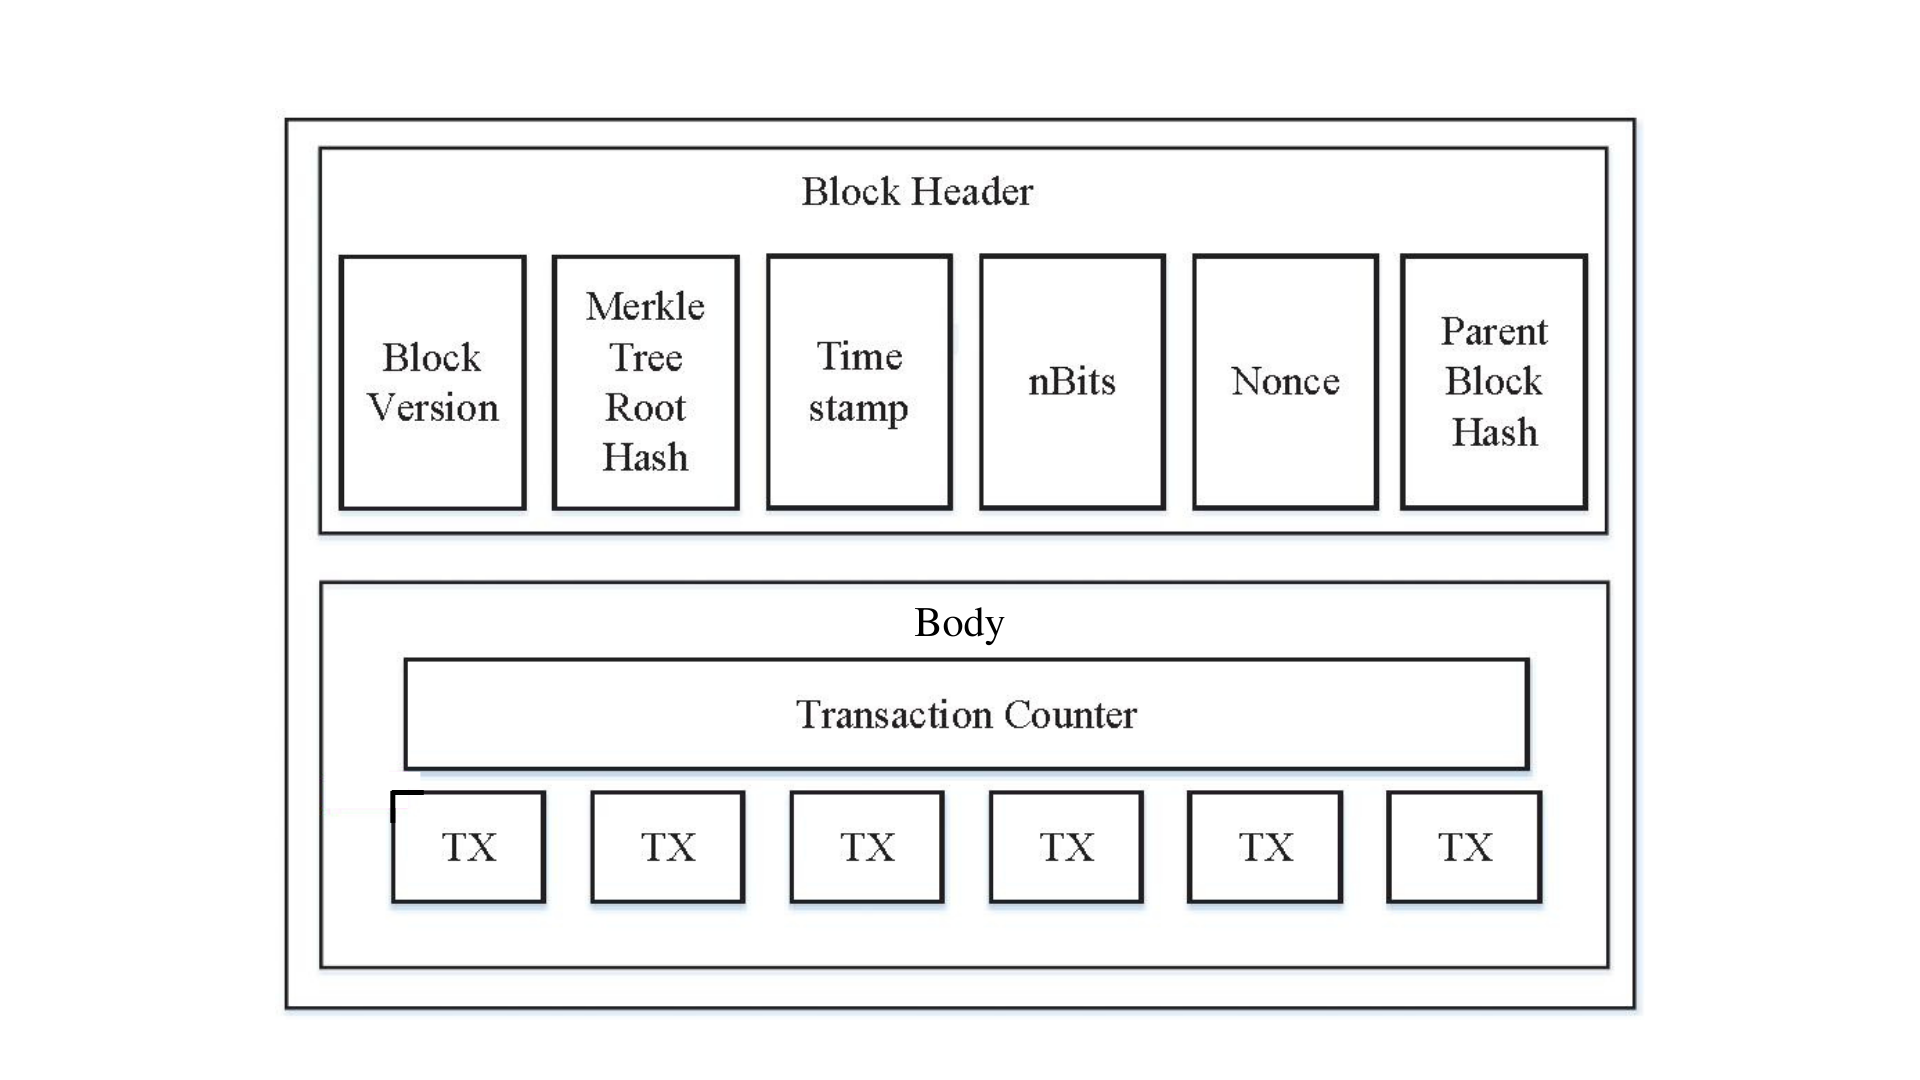
\includegraphics[width=14cm,height=7cm]{Immagini/Struttura_blocco.png}
    \caption[Struttura di un blocco della catena]{Struttura di un blocco della catena.}
    \label{struttura_blocco_img}
\end{figure}
\begin{itemize}
    \item La \textit{versione}, la quale indica le regole di \textit{validazione del blocco}\footnote{L'operazione di validazione del blocco è l'elemento essenziale della Blockchain, permette l'aggiunta del blocco alla fine della catena dopo una serie di verifiche e controlli che verranno approfonditi in (\ref{mining}).} da rispettare. Esse dipendono dalla versione del software che viene utilizzato per una specifica Blockchain;

    \item Il \textit{Parent Block Hash}(o \textit{Previous Hash}) è un valore di 256 bit riferito al blocco precedente della catena. Se il valore hash del blocco precedente a cui è riferito cambia, anche il PreviousHash cambierà, innescando, così, una reazione a catena di aggiornamento di identità tra tutti i blocchi successivi al blocco modificato. Verrà approfondito in (\ref{hashing});
    \item Il \textit{Merkle Tree Root Hash} è una struttura dati con diversi use-case. Uno dei principali è quello di garantire l'integrità dei dati usufruendo dell'hashing. Verrà approfondito in (\ref{Merkle_Tree});
    \item Il \textit{timestamp}, letteralmente “marca temporale”, rappresenta un preciso istante, con lo scopo di accertare l’effettivo avvenimento di un determinato evento;
    \item Il campo \textit{Bits}(o \textit{difficulty target}) è la soglia \textit{target} calcolata dall'algoritmo Proof-Of-Work di un hash di blocco valido;
    \item Il campo \textit{Nonce} è un valore in byte, aggiunto al blocco e ricalcolato tramite \textit{rehashing}\footnote{Procedura che identifica delle operazioni di \textit{hashing} ripetute nel tempo.} in maniera tale che quest'ultimo rispetti dei criteri per la validazione del blocco. Questa operazione necessita di una grande potenza di calcolo; si tratta del famoso \textit{mining}, approfondito in (\ref{mining}).
\end{itemize}

Il \textit{body} del blocco, invece, è composto da un \textit{contatore di transazioni} e dalle transazioni vere e proprie (indicate come “TX” nella figura \ref{struttura_blocco}). Queste transazioni devono essere \textit{verificate}\footnote{La verifica di una transazione consiste nella conferma dei dettagli della transazione, inclusi il tempo della transazione, l’importo e i partecipanti.}. Il funzionamento e la logica delle transazioni verrà approfondito in (\ref{transazioni}).
\subsection{L'hashing per il collegamento dei blocchi} \label{hashing}
\begin{figure}[h]
    \centering
    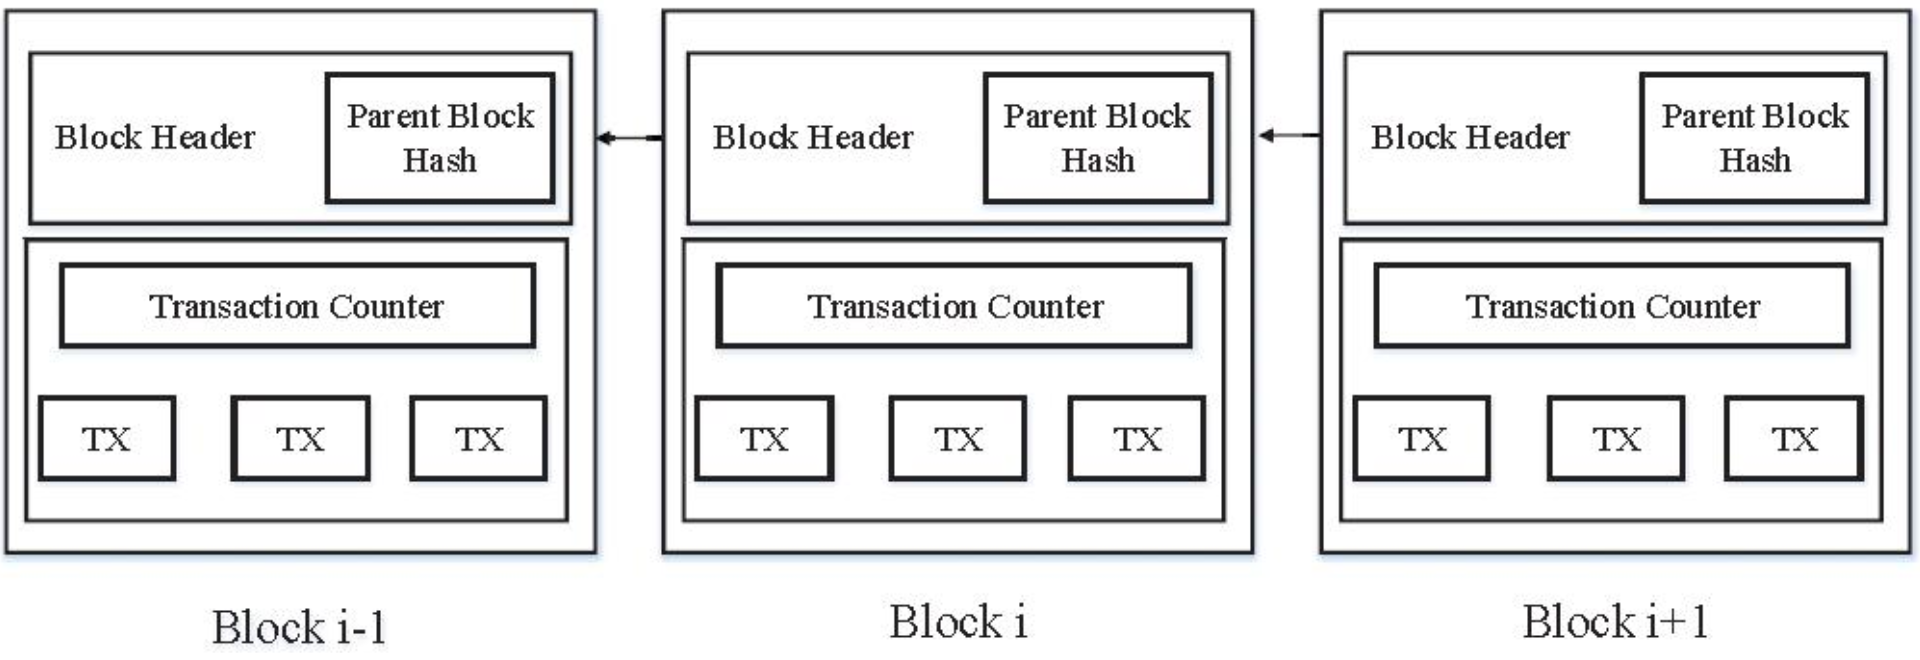
\includegraphics[width=12.5cm,height=5cm]{Immagini/Catena.png}
    \caption[Schema base di una catena di blocchi]{Schema base di una catena di blocchi (Blockchain).}
    \label{catena}
\end{figure}
Come accennato, la Blockchain è una struttura dati formata da una serie di blocchi collegati tra di loro(un esempio di schema base viene mostrato in figura \ref{catena}).
I nuovi blocchi si formano quando i partecipanti della rete creano nuovi dati o aggiornano quelli già esistenti. Questi blocchi memorizzano dei dati crittografati e dotati di un ID\footnote{Abbreviazione di “Identificativo”.} univoco, chiamato Hash.
Nella Blockchain l’hash è il collante che tiene insieme i blocchi, creando, a tutti gli effetti, una \textit{catena di blocchi}. L'hash rende questa catena a prova di manomissioni garantendo l'integrità e l'autenticità dei dati presenti in ogni singolo blocco. In questo paragrafo introdurremo il funzionamento dell'hashing in generale e l'utilizzo specifico per la tecnologia Blockchain.

Per hashing si intende il processo nel quale una qualsiasi chiave k viene inserita in una \textit{funzione di hash} h in modo da ottenere un intero\footnote{In informatica, un intero viene definito come un tipo di dato utilizzato per rappresentare numeri reali che non hanno valori frazionari.} h(k). La coppia chiave-valore \lstinline|<k,v>| viene memorizzata in un vettore (detto \textit{tabella di hash}) nella posizione h(k).
Una funzione hash è definita come:

\begin{equation*}
    h:U \rightarrow  \{0,1,...,m-1\} , dove:
\end{equation*}

\begin{itemize}
    \item \textit{h}, come anticipato, è la funzione di hash;
    \item \textit{U} è l'insieme Universo (insieme delle possibili chiavi);
    \item \textit{m} $\in \mathbb{N}$ è la dimensione del vettore T;
    \item \textit{T} è la tabella di hash nel quale vengono memorizzate le coppie chiave-valore.Un esempio lo si mostra in \ref{tabella_hash}.
\end{itemize}
\begin{figure} [h]
    \centering
    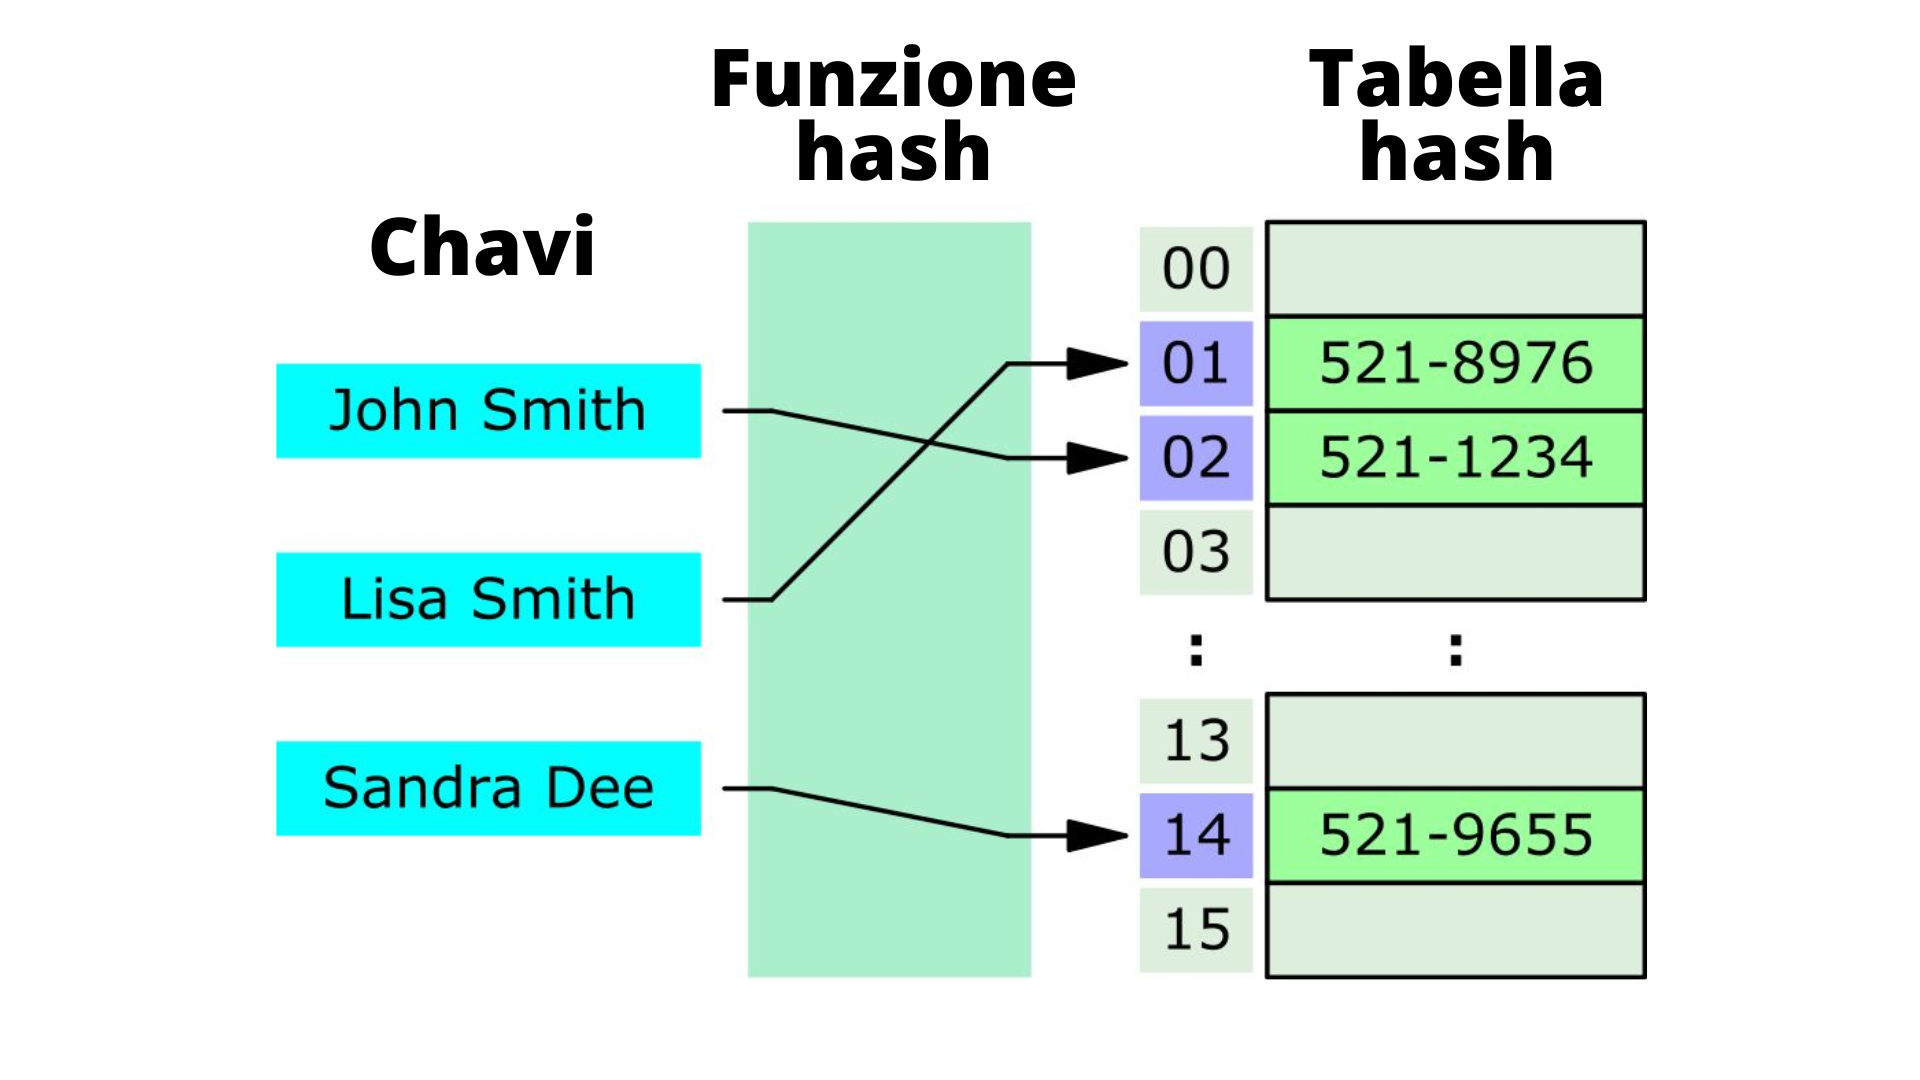
\includegraphics[width=12cm,height=5cm]{Immagini/Chavi.png}
    \caption[Esempio di tabella hash]{Esempio di tabella hash.}
    \label{tabella_hash}
\end{figure}

Nell'ambito Blockchain si utilizzano le \textit{funzioni crittografiche di hash}, le quali, non sono altro che una categoria speciale delle funzioni di hash classiche. Queste particolari funzioni devono:

\begin{itemize}
    \item essere \textit{deterministiche} (cioè ogni messaggio possiede il sempre lo stesso hash);
    \item rendere univoco il valore di hash per ogni input;
    \item rendere molto difficile poter generare un messaggio da un dato valore di hash;
    \item essere veloci nel calcolare il valore di hash.
\end{itemize}.  
Queste caratteristiche peculiari delle \textit{funzioni crittografiche di hash} le rendono particolarmente adatte per garantire l'integrità, l'autenticità e la sicurezza dei dati.

Applicate al contesto Blockchain, l'hash è ciò che conferisce l'unicità al singolo blocco. Ogni blocco della catena dipende dal precedente, poiché, nel pacchetto di dati di ognuno di essi, è incluso l’hash del blocco antecedente ad esso; ciò comporta l'alterazione di tutti i blocchi successivi, ogniqualvolta, un dato blocco viene modificato dopo la registrazione iniziale dei dati per quest'ultimo.
Come anticipato in (\ref{struttura_blocco}), ogni blocco possiede un \textit{timestamp}, che, esattamente come gli altri componenti, influenza inevitabilmente il valore hash del blocco e, come si dice in \cite{bitcoin}:“[...] prova che i dati devono essere esistiti in quella determinata data, dal momento che sono finiti nell'hash.[...]”.

Oggigiorno esistono diverse \textit{funzioni crittografiche di hash} ma col passare degli anni è stato dimostrato che alcune di esse non sono molto sicure e possiedono diverse vulnerabilità.
La funzione di hash più utilizzata in ambito Blockchain è la \textit{Secure Hash Algorithm} (SHA). Negli anni sono state segnalate collisioni e vulnerabilità per la famiglia degli SHA-0 e SHA-1, rendendoli, così, poco consigliati all'uso.
Ultimi studi hanno dimostrato che le nuove applicazioni possono evitare questi problemi utilizzando le versioni più recenti degli SHA.
La \textit{funzioni crittografiche di hash} utilizzata per il Bitcoin è la SHA-256 (della famiglia degli SHA-2), la quale possiede un \textit{digest}\footnote{Un message digest è una rappresentazione numerica a dimensione fissa del contenuto di un messaggio, calcolata da una funzione hash.} di 256 bit.\\
Per quanto riguarda Ethereum, prima del recentissimo aggiornamento del 15 Settembre di quest'anno al “The Merge”\cite{TheMerge} (un piano di aggiornamento pensato diversi anni fa per migliorare la scalabilità, la sicurezza e la sostenibilità della rete Ethereum, senza compromettere la sua decentralizzazione. Si è passati al meccanismo di consenso Proof-Of-Stake (PoS)\footnote{PoS è un algoritmo di consenso nel quale, ad ogni utente, viene richiesto il possesso di un certo quantitativo di criptovaluta. I \textit{miners} vengono scelti in base alla loro ricchezza e non alla loro potenza di calcolo; questa peculiarità rende la PoS sostenibile e priva di enormi fabbisogni energetici.}.), la \textit{funzione crittografica di hash}  che veniva utilizzata era il Kekkak-256, esso possiede un \textit{digest} arbitrario. Sottoinsieme della famiglia dei Kekkak è lo SHA-3 , ultima versione della famiglia di standard SHA. 
\subsection{Transazioni:il meccanismo della Digital Signatures Chain} \label{transazioni}

Nella Blockchain le transazioni servono per scambiare asset di qualsiasi natura tra due o più soggetti devono essere mantenute da ogni individuo della rete e rese pubbliche tramite un messaggio broadcast.
In un contesto decentralizzato, ogni transazione ha lo stesso valore d'importanza rispetto ad un'altra, di conseguenza, come è stato già anticipato in (\ref{1.2}), tutti gli utenti della rete devono verificare la suddetta transazione garantendo l'autenticità della stessa.
Una soluzione viene proposta da Satoshi Nakamoto in \cite{bitcoin}: ossia quella di un sistema di \textit{firme digitali}.
Ogni nodo nella rete Peer-to-Peer (P2P) della Blockchain possiede una \textit{chiave pubblica} e una \textit{chiave privata}:

\begin{itemize}
    \item La \textit{chiave pubblica} è un valore, talvolta identificato come indirizzo, che tutti gli utenti della rete conoscono;
    \item La \textit{chiave privata} è un indirizzo univoco che solo l'utente possessore ne è a conoscenza.
\end{itemize}

Per mettere in atto il sistema delle \textit{firme digitali}, ogni transazione emessa viene firmata digitalmente utilizzando il valore hash (il modo con cui viene generato è spiegato in \ref{hashing}) e la chiave privata riferita al mittente.
L'output generato verrà trasmesso in tutta la rete usando la chiave pubblica del destinatario della transazione. Solo il destinatario, unico possessore della chiave privata riferita alla sua chiave pubblica, potrà decifrare il messaggio criptato;  così facendo è possibile anche verificare l'autenticità della transazione verificando la firma digitale generata. \\
Una volta che l'autenticità delle transazioni viene verificata è doveroso analizzare la maniera con cui le transazioni vengono memorizzate all'interno dei blocchi.
Le transazioni vengono memorizzate all'interno di un blocco grazie al concetto di \textit{Digital Signatures Chain} (o catena di firme digitali), il quale funzionamento, come viene espresso in \cite{bitcoin} definisce un meccanismo per il quale :“[...]ciascun proprietario, al momento della transazione, firma digitalmente un hash della transazione precedente e la chiave pubblica del proprietario successivo[...]”. 
Questa procedura permette di creare una vera e propria catena di transazioni (similmente alla catena di blocchi, una struttura dati) salvata all'interno di ogni blocco della Blockchain; un'illustrazione grafica la si mostra in figura \ref{transaction_chain}.\\
\begin{figure}[h]
    \centering
    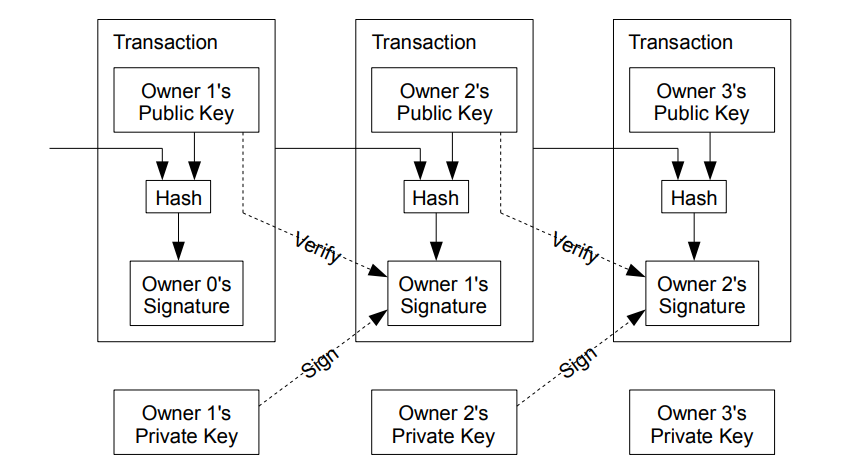
\includegraphics[width=12cm,height=7cm]{Immagini/Transaction_Chain.png}
    \caption[Transaction Chain]{Transazioni memorizzate in un blocco tramite il meccanismo di \textit{Digital Signatures Chain}.}
    \label{transaction_chain}
\end{figure}
Come mostrato in (\ref{struttura_blocco}), all'interno del body di ogni blocco sono presenti diverse transazioni. Queste transazioni sono incluse a loro volta in diverse catene di transazioni; queste ultime permettono di tenere traccia di tutte
le operazioni finanziarie a cui sono stati sottoposti i fondi digitali di tutti i partecipanti. Come affermato nel whitepaper di Bitcoin \cite{bitcoin} ,tutto ciò è definibile come una \textit{moneta digitale}(o elettronica).

\subsection{I Merkle Trees Root e l'integrità dei dati}\label{Merkle_Tree}
Un'altra componente che garantisce l'integrità dei dati presenti in un blocco è il \textit{Merkle Tree}, il quale non è altro che una struttura dati ad \textit{albero}\footnote{Un albero è una struttura dati composta da nodi collegati da archi, creando una gerarchizzazione dei dati presenti al  suo interno.} memorizzata, sotto forma di singola radice (Merkle Tree Root), nell'\textit{header} del blocco(come anticipato in \ref{struttura_blocco}).
Il \textit{bottom layer} di questa struttura ad albero , come viene espresso in un articolo scientifico sul tema \cite{merkle_tree}: “[...] mostra le transazioni memorizzate (ad es. T001 come mostrato in figura \ref{merkle_root_img}) per il blocco, che in seguito vengono convertite nelle loro firme hash SHA256 (ad es. H001 come mostrato in figura \ref{merkle_root_img}) e rappresentano le foglie dell'albero di Merkle.[...]”.

\begin{figure}[h]
    \centering
    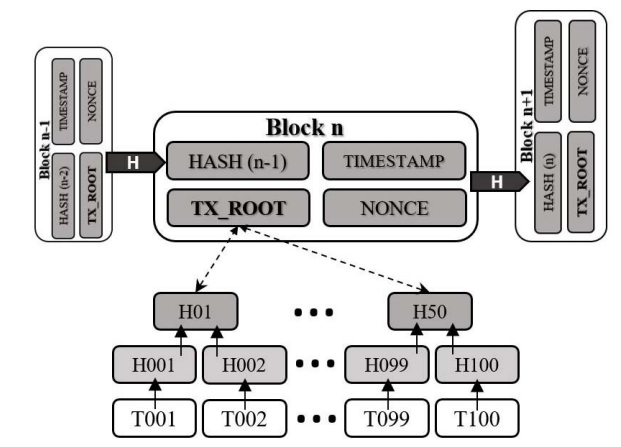
\includegraphics[width=12cm,height=8cm]{Immagini/Merkle_Tree.png}
    \caption[Merkle Tree Root]{Merkle Tree Root memorizzato nell'header di un blocco.}
    \label{merkle_root_img}
\end{figure}
I calcoli della radice di Merkle Tree vengono effettuati attraverso il calcolo dell'hash \textit{ricorsivamente}\footnote{In maniera ricorsiva, ossia espresso in termini di sé stesso.} a partire dalle foglie. Una volta trovato l'hash “finale”, esso rappresenterà la radice del Merkle Tree (definita come TX\_ROOT in figura \ref{merkle_root_img}).

Pertanto, se anche solo un nodo nell'albero venisse modificato, la variazione dei valori hash si diffonderebbe fino alla radice, rendendola immediatamente identificabile. La Merkle Root viene quindi utilizzata per verificare che i blocchi ricevuti dagli altri nodi siano intatti e che nessuna transazione passata sia stata alterata.


\subsection{Il mining per la validazione dei blocchi}\label{mining}
Una volta capito come viene verificata l'autenticità di una transazione, è doveroso sapere come vengono \textit{validate} una o più transazioni. Come anticipato, le transazioni devono essere condivise agli altri nodi della rete (\textit{broadcast}) per essere verificate.
Nel Bitcoin mining , esistono dei \textit{nodi validatori}( i cosidetti \textit{miners}\footnote{I miners sono proprietari di computer che contribuiscono con la loro potenza di calcolo e la loro energia alla rete di una criptovaluta basata sulla Proof-Of-Work}), i quali, una volta ricevute le nuove transazioni attualmente in sospeso, ancora non validate, suggeriscono alla rete quale debba essere il nuovo blocco da pubblicare sul network.
Questi \textit{miners} per validare le transazioni e aggiungerle ad un nuovo blocco, creandolo, devono (come anticipato in \ref{struttura_blocco}) calcolare un valore specifico, chiamato \textit{Nonce}, in maniera tale da soddisfare una particolare proprietà; ricordiamo, inoltre, che ogni valore presente all'interno del blocco che viene modificato, a sua volta modificherà anche il valore hash riferito al blocco stesso.
Il calcolo dei miners che richiede un così grande impegno computazionale è proprio quello di generare uno specifico hash modificando il valore \textit{Nonce} attraverso complessi problemi matematici.

Ogni blocco, dunque, insieme allo storico delle transazioni, dovrà possedere un determinato hash per essere considerato valido a tutti gli effetti ( in Bitcoin, per esempio, il criterio è quello di generare un certo numero di zeri all'inizio del valore hash riferito al blocco). 
Solo i primi minatori che riescono a risolvere il problema vengono ricompensati da una quota di Bitcoin, generata proprio grazie a questo processo.
Ciò significa che coloro i quali possiederanno maggiori risorse computazionali avranno maggiori probabilità di acquisire il “bottino” (block reward \footnote{La ricompensa data ai miners ogni qualvolta viene “minato” un blocco.}) rispetto agli altri. 

Infine, il blocco viene aggiunto alla Blockchain, incrementandone la lunghezza, e le transazioni in esso contenute arrivano a destinazione.
\section{Evoluzione della Blockchain}
In questo capitolo si analizzerà la storia e l'evoluzione di questa tecnologia, si esamineranno tutte le funzionalità che, nel corso degli anni, sono state aggiunte alla Blockchain, partendo dagli albori.

Tratteremo tre diverse varianti:
\begin{itemize}
\item La Blockchain 1.0 : Bitcoin come moneta elettronica peer-to-peer (\ref{Blockchain1.0});
\item La Blockchain 2.0 : Ethereum e l'introduzione agli smart-contract (\ref{Blockchain2.0});
\item La Blockchain 3.0 : Dapp e Blockchain applicata all'industria 4.0 (\ref{Blockchain3.0});
\end{itemize}
\subsection{Blockchain 1.0 : Bitcoin come moneta elettronica peer-to-peer}\label{Blockchain1.0}
Blockchain 1.0 rappresenta la prima applicazione della tecnologia,  implementata da Satoshi Nakamoto, come accennato all'inizio del capitolo \ref{cap1}. 
Questa versione è la configurazione più semplice di registro distribuito (DLT) per la registrazione di transazioni e la memorizzazione dei dati su più computer. La Blockchain di Bitcoin si limita al trasferimento di denaro tra gli utenti senza il bisogno di avere un'autorizzazione esterna(quindi senza intermediazione tra le operazioni finanziarie). Al contempo, le sue caratteristiche (che abbiamo precedentemente conosciuto) ne accentuano il ruolo di potenziale riserva di valore.
\begin{figure}[h]
    \centering
    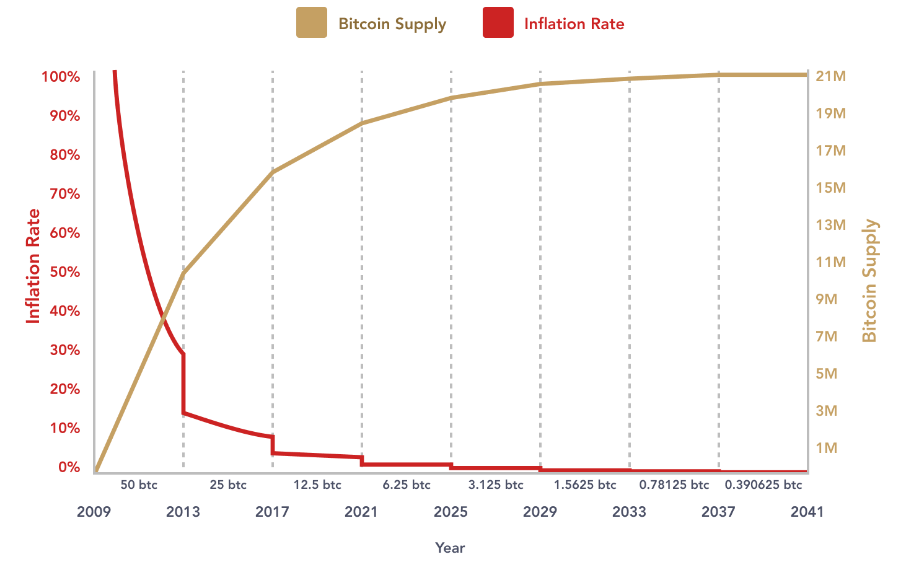
\includegraphics[width=13cm,height=7cm]{Immagini/halving.png}
    \caption[Grafico del tasso inflattivo e della supply di Bitcoin]{Andamento del tasso inflattivo e della \textit{supply} di Bitcoin nel corso del tempo.}
    \label{grafico_inflazione_btc}
\end{figure}
\subsubsection{Come ha fatto Bitcoin a diventare così famoso nel mondo?}
I suoi clamorosi aumenti di valori nel corso della storia e la sua politica monetaria a inflazione\footnote{L'inflazione è il processo in seguito al quale le valute perdono valore nel tempo, causando un aumento dei prezzi dei beni di consumo.} decrescente e \textit{programmata} ha reso famoso Bitcoin facendo parlare di sé e della sua tecnologia in tutto il mondo.
Per capire al meglio come faccia il sistema ad avere una politica deflattiva, introduciamo il concetto di \textit{halving}, ossia quella procedura che dimezza del 50\% la creazione di nuovi Bitcoin ogni 210000 blocchi “minati”(circa ogni 4 anni considerando che il tempo di mining per il singolo blocco è di 10 minuti). La ricompensa iniziale, al momento della pubblicazione di Bitcoin, era di 50 BTC\footnote{Abbreviazione di Bitcoin.} per blocco, ma se questa ricompensa fosse rimasta la stessa, la valuta in circolazione sarebbe aumentata infinitamente nel corso del tempo e si sarebbe verificato, di conseguenza, una continua inflazione. Per evitare questo problema il sistema è stato \textit{programmato} per raggiungere una \textit{max supply}\footnote{La Maximum Supply (offerta totale) di una criptovaluta è la fornitura massima di monete che verranno mai generate.} di 21 milioni di unità.
Il sistema, grazie all'\textit{halving}, quindi, rende Bitcoin più scarso col passare del tempo aumentando il suo prezzo(si evidenzia come Bitcoin sia un asset di natura deflattiva\footnote{Fenomeno opposto all'inflazione, quindi una diminuzione generalizzata dei prezzi, che genera un incremento del potere d'acquisto della moneta.} in figura \ref{grafico_inflazione_btc}). Di seguito si mostra il calcolo per il raggiungimento della \textit{max supply}.
\begin{equation*}
\sum\limits_{i=0}^{32}  210000 \cdot \frac{50}{2^i}       ,dove:
\end{equation*}
\begin{itemize}
\item la variabile \textit{i} rappresenta il numero di \textit{halving} (partendo da zero fino ai 32 \textit{halving} stimati per il futuro);
\item \textit{210000} sono i numeri di blocchi da minare (il processo di mining viene spiegato in \ref{mining}) per fare in modo che si passi all'\textit{halving} successivo e si incrementi la variabile i;
\item il valore \textit{50} corrisponde, come anticipato, alla ricompensa iniziale di BTC per ogni blocco minato. Quest'ultimo viene diviso per \textit{$2^i$} volte.
\end{itemize}

Logicamente, una ricompensa sempre più bassa comporta meno generazione di moneta e di conseguenza un maggior tempo per raggiungere la \textit{max supply}, di fatto, la data stimata in cui verrà raggiunta si aggira intorno al 2140.

Possiamo sintetizzare la prima generazione di Blockchain come l'innesco che ha dato il via alla rivoluzione degli scambi peer-to-peer monetari. L'interesse mondiale verso Bitcoin ha posto le basi per lo studio di nuovi possibili sviluppi e use-case per questa tecnologia.
\subsection{ Blockchain 2.0 : Ethereum e la programmabilità della Blockchain tramite smart-contract (DeFi e Dapp)}\label{Blockchain2.0}
La seconda generazione di Blockchain è rappresentata da Ethereum\footnote{Da: \cite{ethereum_definizione} “Ethereum è una piattaforma decentralizzata del Web 3.0 per la creazione e pubblicazione peer-to-peer di contratti intelligenti[...]. La criptovaluta legata ad essa è Ether. Descritta per la prima volta in \cite{ethereum}.} \cite{ethereum}.
Dopo il rilascio di Bitcoin, la Blockchain ha conquistato rapidamente la fantasia degli sviluppatori di tutto il mondo. Nel 2013 (circa 4 anni dopo l'ascesa di Bitcoin) un ragazzo di appena 19 anni di nome Vitalik Buterin\footnote{Sviluppatore di origini russe, ideatore di Ethereum.} propone ad un team di sviluppatori un whitepaper. Dopo aver approvato la sua idea, questi sviluppatori cominciano a lavorare insieme a Vitalik per definire gli ultimi dettagli. L'anno successivo (nel 2014) viene presentato ufficialmente alla North American Bitcoin Conference a Miami il whitepaper finale di Ethereum \cite{ethereum}, rivoluzionando la visione di questa tecnologia nel mondo.

L'idea alla base di Ethereum è quella di creare un grande sistema decentralizzato, che vada oltre il fatto di essere un semplice mezzo di pagamento o un modo per trasferire denaro, e che renda la sua struttura programmabile in toto, dall'automatizzazione degli scambi monetari a veri e propri applicativi decentralizzati.

Per rendere tutto questo possibile, sono stati introdotti gli \textit{smart-contract}(o contratti intelligenti): programmi informatici o codici archiviati nella Blockchain che vengono eseguiti quando vengono soddisfatte condizioni predeterminate.
In Ethereum gli  \textit{smart-contract} sono scritti in Solidity(linguaggio di programmazione approfondito al capitolo \ref{cap2}), uno degli strumenti cardine per lo sviluppo dell'applicazione che verrà mostrata in questo elaborato. 

Il codice degli \textit{smart-contract} viene eseguito in un ambiente chiamato \textit{Ethereum Virtual Machine} (EVM), utilizzato da Ethereum, oltre che per rendere possibile la corretta esecuzione dei codici, anche per implementare tutte quelle funzionalità aggiuntive in maniera tale da mettere in piedi un ecosistema vero e proprio.


In una famosa pubblicazione di \textit{Apress}, nella quale viene introdotto lo studio di Ethereum e della programmazione smart-contract \cite{EthereumBook}, viene affermato quanto segue:“Ethereum cerca di creare un sistema in cui i modelli economici possono essere provati e dimostrati. Per il momento, Solidity sembra destinato a diventare il linguaggio de facto di tali modelli, a condizione che vengano eseguiti su una macchina virtuale globale come l'EVM.”.

Di fatto, riconosce il potenziale di Solidity e degli \textit{smart-contract}, i quali, venendo eseguiti in ambiente Blockchain, ne ereditano tutti i vantaggi, tra cui:

\begin{itemize}
\item Sicurezza:La Blockchain in cui viene registrato il codice informatico del contratto intelligente non consente di essere manomesso e garantisce che possa essere eseguito in modo affidabile,generando risultati sempre verificabili e immutabili;
\item Trasparenza: I record crittografati delle transazioni sono condivisi tra i partecipanti;
\item Risparmio: I contratti intelligenti eliminano la necessità per gli intermediari di gestire le transazioni e, per estensione, i ritardi e le commissioni associati.
\end{itemize}

I contratti intelligenti consentono a due parti di eseguire automaticamente attività molto complesse facilitando lo scambio di valuta digitale, ereditando tutti i vantaggi della Blockchain.

In definitiva, la Blockchain 2.0 ha aperto le porte ad un'infinità di possibili implementazioni e applicazioni.
Tra le più importanti ricordiamo la DeFi, argomento vertice dell'elaborato, spiegato di seguito.

\subsubsection{Decentralized Finance (o DeFi)} 
La \textit{Decentralized Finance} (o DeFi) è uno degli argomenti più discussi nelle comunità Blockchain; essa propone di disintermediare modelli finanziari tradizionali eliminando entità centrali(come banche, istituti di credito, ecc...) dando la possibilità di erogare ed usufruire di servizi finanziari in maniera del tutto decentralizzata. Questi servizi finanziari vengono erogati dalle {Decentralized Application}\footnote{Applicazioni che hanno il proprio codice di back-end in esecuzione su una rete peer-to-peer decentralizzata e ciò la differenzia della maggior parte delle comuni applicazioni il cui codice di back-end è in esecuzione su server centralizzati.} (o Dapp) , ossia delle web-application basate su reti P2P che sfruttano le potenzialità della Blockchain.

Come le normali applicazioni, le Dapp sono composte da un front-end\footnote{La parte visibile all'utente di un programma e con cui egli può interagire.}, un back-end\footnote{La parte non visibile all'utente di un programma che gestisce le funzioni dell'applicazione “dietro le quinte”.} e da un database (in questi casi è la Blockchain o gli smart-contract a fare da database).
La particolarità di queste applicazioni è che, sfruttando la Blockchain, i dati inseriti dagli utenti vengono memorizzati su un registro distribuito in maniera del tutto automatica, grazie all'utilizzo degli \textit{smart-contract} precedentemente introdotti.

Le applicazioni DeFi sono divisi il 5 livelli distinti, come definito in \cite{DeFi_article}:
\begin{itemize} 
 \item Il primo livello è il \textit{settlement layer} (o livello dei regolamenti) in cui vengono regolate tutte le transazioni. Su questo livello si trova la Blockchain e il suo relativo asset nativo ( ad esempio, Ether per la Blockchain di Ethereum).
 La Blockchain, come si dice in \cite{DeFi_article}:“può essere vista come la base per l'esecuzione senza fiducia e serve come livello di risoluzione delle controversie.”;
 \item Il secondo livello è l'\textit{asset layer}. In questo livello sono presenti tutti gli asset emessi dal livello di regolamento, solitamente indicati come token, fungibili\footnote{Un token si dice fungibile quando può essere duplicato un numero infinito di volte in copie identiche e intercambiabili.} e non fungibili come gli NFT(acronimo di Not-Fungible-Token ,anche chiamati “certificati digitali”, da \cite{NFT_definizione} sono: “asset crittografici su una Blockchain con codici di identificazione e metadati unici che li distinguono gli uni dagli altri. Essi non possono essere scambiati in modo equivalente.”);
 
 \item Il terzo livello è il \textit{protocol layer} (o livello dei protocolli), tale livello contiene un insieme di regole e standard concordati che normano le transazioni. Queste regole e standard sono implementati da una serie di \textit{smart-contract};
 \item Il quarto livello è l'\textit{application layer} (o livello di applicazione), il livello nel quale si posiziona l'applicazione implementata per questo elaborato.
 Di fatto, l'\textit{application layer} crea applicazioni che si collegano ai protocolli tramite l'\textit{interazione agli smart-contract}, rendendo i protocolli molto più facili da usare;
 \item Il quinto livello, infine, è l'\textit{aggregation layer} (o livello di aggragazione) il quale fornisce strumenti per la comparazione e la valutazione dei servizi, consentendo agli utenti di svolgere attività altrimenti complesse.
 \end{itemize}

Si mostra in figura \ref{defi_img} una rappresentazione grafica della struttura di un'applicazione DeFi. 

\begin{figure}[h]
    \centering
    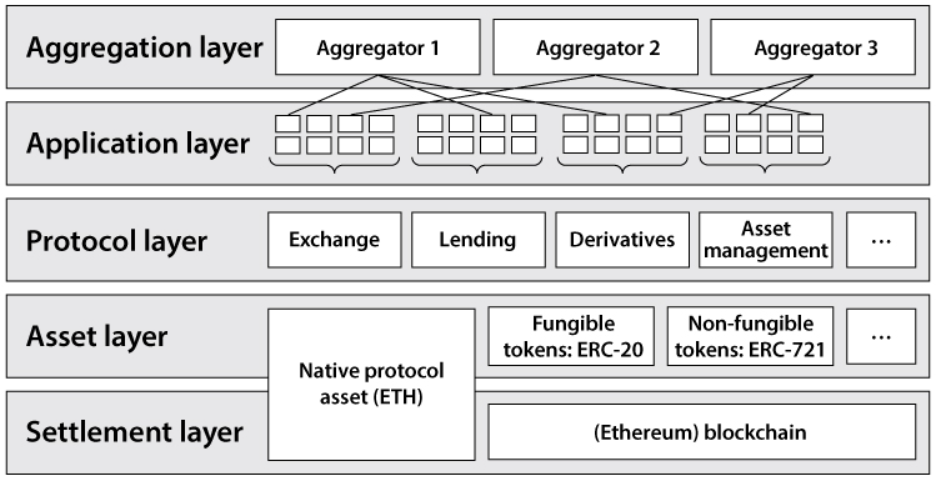
\includegraphics[width=12cm,height=8cm]{Immagini/Defi.png}
    \caption{Struttura di un'applicazione DeFi.}
    \label{defi_img}
    \label{fig:The DeFi Stack}
\end{figure}
\subsection{Blockchain 3.0 : Blockchain applicata all'industria 4.0}\label{Blockchain3.0}
Gli sviluppi successivi alla Blockchain 2.0 non hanno una definizione molto chiara, trattandosi di argomenti in continuo sviluppo.
Oggi come oggi, potremmo comunque definire la Blockchain 3.0 come quell'ondata evolutiva che cerca di oltrepassare e ottimizzare i servizi delle prime due generazioni, rendendo, al contempo, la tecnologia Blockchain utilizzabile per le esigenze aziendali.
Sopratutto riferiti all'industria 4.0, la quale, in breve, non è altro che, come viene detto in \cite{industria4.0}:“la propensione dell'odierna automazione industriale ad inserire alcune nuove tecnologie produttive per migliorare le condizioni di lavoro, creare nuovi modelli di business, aumentare la produttività degli impianti e migliorare la qualità dei prodotti. [...]”.
Questa particolare rivoluzione industriale richiede (come d'altronde in generale nel prossimo futuro) un grado sempre più alto di sicurezza della privacy e dei dati e maggiore fiducia. Qui entra in gioco la Blockchain.

Le principali preoccupazioni per questa generazione di Blockchain sono la sostenibilità, la scalabilità, l'economicità, una maggiore decentralizzazione e una maggiore sicurezza.

La sostenibilità, che è un argomento di forte attualità, influenza le scelte delle nuove famiglie di Blockchain. Molte Blockchain, come è stato già anticipato nei capitoli precedenti, necessitano di grandi potenze di calcolo per alcune operazioni ( si pensi, per esempio, al mining) comportando un grande dispendio energetico. Non a caso le Blockchain si stanno aggiornando tenendo in considerazione questo fattore( basti guardare al Merge di Ethereum \cite{TheMerge}), passando a modelli più sostenibili come il Proof-Of-Stake (PoS).

%La Blockchain 3.0 ,inoltre, deve essere capace di integrare e supportare altri contesti applicativi come quelli dell'\textit{Internet of Things}\footnote{Da \cite{IoT} :”neologismo utilizzato nel mondo delle telecomunicazioni e dell'informatica che fa riferimento all'estensione di internet al mondo degli oggetti e dei luoghi concreti, che acquisiscono una propria identità digitale in modo da poter comunicare con altri oggetti nella rete e poter fornire servizi agli utenti.”}(Iot) o dell' \textit{Intelligenza Artificiale}\footnote{L'intelligenza artificiale, anche chiamata IA, come detto in \cite{IA} è :”una disciplina che studia se e in che modo si possano realizzare sistemi informatici intelligenti in grado di simulare la capacità e il comportamento del pensiero umano.[...]”}, puntando sempre di più sulle Dapp.


In conclusione, al netto di tutti questi incredibili possibili sviluppi, la tecnologia Blockchain ha ancora molto da offrire al mondo che verrà, rendendola, di fatto, una delle tecnologie più interessanti da approfondire.
%%%%%%%%%%%%%%%%%%%%%%%%%%%%

%%%%%%%%%%%%%%%%%%%%%%%%%%%%

\chapter{Strumenti di sviluppo}\makeatletter\def\@currentlabel{2}\makeatother
\label{cap2}
\lhead{\textbf{CAPITOLO 2.} \textit{ STRUMENTI DI SVILUPPO}}

\section{Organizzazione dell'applicativo}\label{Organizzazione}
Una volta compreso il funzionamento e le peculiarità della tecnologia Blockchain, ci indentriamo nello sviluppo vero e proprio dell'applicazione.
Come anticipato, l'applicazione è una Dapp DeFi strutturata sulla rete Ethereum (per la precisione sulla rete di test Ropsten.); composta da un front-end in React e un back-end formato da smart-contract (memorizzati su Blockchain) scritti in Solidity, il quale, ci consente di distribuire l'applicazione sia su mainnet Ethereum che su qualsiasi altra Blockchain EVM compatibile. In questo capitolo verrà mostrato come le due controparti sono collegate tra di loro e tutte le tecnologie specifiche utilizzate.

\section{Tecnologie per il back-end}\label{back-end}
In una Dapp, gli smart-contract “sostituiscono” il back-end delle applicazioni tradizionali per evitare i server centralizzati e agire in modo distribuito (P2P),invece che utilizzare il protocollo HTTP per comunicare.
Gli smart-contract di Ethereum consentono di costruire architetture in cui una rete di contratti si trasmette dati tra loro, leggendo e scrivendo le proprie variabili di stato man mano che procedono, con la loro complessità limitata solo dal solo \textit{block gas limit}\footnote{Il limite di gas definisce il limite superiore del gas destinato al consumo di una transazione o per l'intero blocco.}.
Deve essere, inoltre, considerato che uno smart-contract è impossibile da modificare dopo essere stato distribuito, può soltanto essere cancellato se è stata aggiunta in precedenza una particolare funzione(per la precisione la SELFDESTRUCT opcode\footnote{un'operazione a livello della EVM, indipendente dal tipo di linguaggio o client che stai utilizzando}).

\subsection{Node.js}\label{nodeJS}
Node.js è un ambiente di runtime JavaScript open source usato per eseguire codice JavaScript all'esterno di un browser web. Ai fini del nostro progetto, node.js ci servirà per il Node Package Manager (NPM) come pre-requisito all'installazione di Truffle (\ref{Truffle}), del React App (\ref{React}) e della libreria web3.js (\ref{web3_Library}). 
\subsection{Solidity}\label{Solidity}
Per l'implementazione degli smart-contract su rete Ethereum si utilizza Solidity,  un linguaggio di programmazione object-oriented\footnote{Letteralmente “orientato agli oggetti”. L'object orientation è un paradigma di programmazione che si basa sul concetto di classi e oggetti.} designato specificamente per il loro sviluppo (vengono eseguiti sulla macchina virtuale di Ethereum)\cite{Solidity_docs}. Questo linguaggio (che è di alto livello) è stato pensato per rendere più semplice la scrittura di smart-contract, i quali, devono essere compilati in bytecode EVM (ossia codice di basso livello interpretabile solo dalla macchina e non dall'uomo).

Per fare questo, c'è bisogno di un Contract ABI (o Application Binary Interface), ossia un'interfaccia che permette di interagire con uno smart-contract tramite uno schema standard, definendo i nomi delle funzioni e i tipi di dati degli argomenti. L'ABI, infatti, è scritto in formato JSON\footnote{Acronimo di JavaScript Object Notation, è un formato standard utilizzato per lo scambio e la memorizzazione di dati sottoforma di coppie o array attributo-valore.}.

Nella nostra Dapp, dunque, quando si vogliono inserire o leggere dei dati sulla Blockchain, le funzioni chiamate devono passare sempre per l'ABI che fa da intermediatore con l'EVM. Si mostra in figura \ref{contratti_img} il processo illustrato graficamente.

\begin{figure}[h]
    \centering
    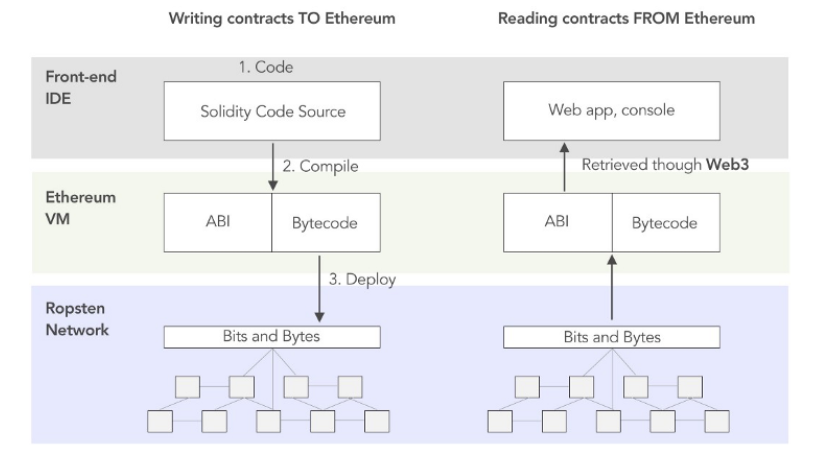
\includegraphics[width=13cm,height=8cm]{Immagini/Contratti_ETH.png}
    \caption[Rappresentazione grafica del processo di lettura/scrittura delle funzioni di uno smart-contract]{Processo di lettura/scrittura delle funzioni di uno smart-contract.}
    \label{contratti_img}
\end{figure}

Un vantaggio di Solidity è che i codici sorgente realizzati sono accessibili pubblicamente nella Blockchain di Ethereum (consultabili su qualsiasi block explorer, ossia: come detto in \cite{block_explorer}: “è uno strumento che fornisce analisi dettagliate su una rete Blockchain[...]”, esso funge da un motore di ricerca  nel quale si possono controllare i singoli blocchi, le transazioni e gli indirizzi pubblici). Per quanto riguarda la visualizzazione di questi codici: se essi sono verificati, viene mostrato il codice sorgente, altrimenti vengono mostrati in bytecode.

Solidity oltre ad essere stato uno dei primi linguaggi di programmazione smart-contract, è il più utilizzato al momento per il suo scopo e viene considerato, inoltre, il più versatile tra tutti.
\subsection{Truffle framework}\label{Truffle}
Durante l'intero ciclo di vita del progetto, è stato utilizzato il framework Truffle della Truffle Suite di Consensys\footnote{Una delle principali aziende di sviluppo software Blockchain di Ethereum.}\cite{Truffle_Suite} per il supporto allo sviluppo e alla distribuzione degli smart-contract permettendo di comunicare con essi, senza faticose programmazioni lato client. Truffle permette diverse funzioni:
\begin{figure}[h]
    \centering
    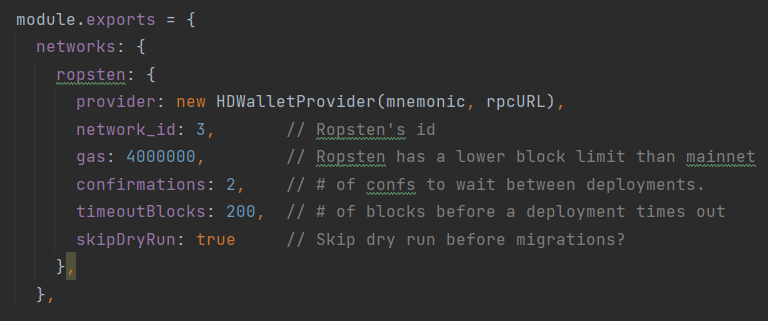
\includegraphics[width=13cm,height=6cm]{Immagini/truffle_config.png}
    \caption[File di configurazione truffle-config.js]{File di configurazione \textit{truffle-config.js} per la testnet Ropsten.}
    \label{truffle_config}
\end{figure}
\begin{itemize}
\item Gestire i propri contratti collegando librerie e diverse applicazioni Ethereum;
\item Automatizzazione del testing dei contratti per uno sviluppo più rapido;
\item Distribuzione e Migrazione degli script. La migrazione aiuta i contratti ad essere distribuiti e salvati sulla rete Ethereum, Truffle gestisce le migrazioni tramite dei file Javascript \footnote{Linguaggio di programmazione multi paradigma orientato agli eventi.}, i quali, da documentazione \cite{Truffle_migration}:“[...]sono responsabili della gestione temporanea delle attività di distribuzione e vengono scritti partendo dal presupposto che le esigenze di distribuzione cambieranno nel tempo.[...]”;
\item Fornisce una console interattiva per compilare, testare o debuggare\footnote{Procedura molto importante che permette di facilitare  la ricerca di errori logici all'interno del programma, viene effettuato attraverso un' altro programma chiamato debugger.} i propri contratti.
\end{itemize}

Truffle distribuisce l'applicazione su un nodo che rappresenta la rete (Blockchain) specifica da voler utilizzare; il tutto viene definito in un unico file Javascript di configurazione chiamato \textit{truffle-config.js}.
Nel nostro caso l'applicazione è stata distribuita sulla rete di test Ropsten di Ethereum, il file di configurazione è mostrato in figura \ref{truffle_config}.

\section{Tecnologie per il Front-end}\label{front-end}
A differenza del back-end, in una Dapp il funzionamento lato front-end e l'interfaccia utente (UI) non cambiano rispetto una web-app tradizionale, l'unica differenza la fa l'interazione con il back-end.
La gestione delle interazioni con la rete Ethereum nell'applicazione vengono assegnate alla libreria Javascript \textit{web3.js} e all'estensione del browser \textit{Metamask} (spiegati nei paragrafi successivi).

\subsection{React}\label{React}
La nostra applicazione è stata realizzata interamente in \textit{React}\cite{React}, una libreria Javascript per la creazione di UI sviluppata nel 2013 da Facebook; la libreria è ora open-source ed è sostenuta da una vasta comunità di programmatori. 
React permette di creare interfacce dinamiche complesse che allo stesso tempo risultano essere semplici e intuitive da utilizzare.

Come è ormai risaputo, per la creazione di applicazioni Web è necessario coinvolgere i tre linguaggi fondamentali:
\begin{itemize}
\item HTML ( o Hypertext Markup Language) per strutturare il sito web;
\item CSS (o Cascading Style Sheets) per la resa grafica dell'applicazione;
\item Javascript, invece, per la logica applicativa e per rendere interattive le applicazioni web.
\end{itemize}

Nelle applicazioni \textit{React}, tutto questo viene semplificato nella sintassi JSX (Javascript XML), un'estensione della sintassi di Javascript, che ci permette di inserire delle strutture simili ad HTML nello stesso file in cui si scrive la logica Javascript. L'uso di JSX, seppur non obbligatorio, permette una più facile lettura degli elementi e dei suoi attributi. Questo particolare tipo di sintassi non è decifrabile nativamente dai browser web e c'è bisogno di un pre-compilatore per rendere leggibile il tutto; la libreria \textit{React}, oggi come oggi, utilizza Babel\footnote{Compiler Javascript.} per questo scopo.

Una delle peculiarità di React è quella di comporre le sue applicazioni di \textit{componenti} riutilizzabili permettendo di semplificare lo sviluppo, di non ripetere frazioni di codice più volte e di importare un determinato componente solo quando è davvero necessario.
Ogni componente può essere personalizzato a proprio piacimento incorporando un CSS specifico.

\subsection{La libreria Web3.js}\label{web3_Library}
Come anticipato nei paragrafi precedenti, la libreria \textit{web3.js}\cite{web3API} viene utilizzata per l'interazione con gli smart-contract su Ethereum.

Come viene espresso in \cite{web3API} web3.js è :“una raccolta di librerie che consentono di interagire con un nodo Ethereum locale o remoto utilizzando HTTP, IPC o WebSocket.”, essa è l'API\footnote{Abbreviazione di Application Programming Interface, è un'interfaccia composta di definizioni e protocolli per la creazione e l'integrazione di software applicativi.} Javascript ufficiale di Ethereum.
Prima di definire nel dettaglio il funzionamento e le caratteristiche di questa libreria, introduciamo brevemente il concetto di JSON-RPC.

JSON-RPC (Remote Procedure Call Protocol) è un protocollo per la chiamata di procedure remote,  nelle quali è possibile passare anche oggetti complessi e ricevere come output dati multipli. I codici di successo e di errore sono standardizzati, in maniera tale da renderne più facile la comprensione.

Questo servizio viene interrogato tramite HTTP o TCP/IP e restituisce una serializzazione del risultato in formato JSON. Ogni richiesta è caratterizzata dalle seguenti componenti:
\begin{itemize}
\item method: Stringa contenente il nome del metodo che la richiesta deve invocare;
\item params: Corrisponde ai parametri da passare al metodo sotto forma di array di oggetti;
\item id: un valore univoco utilizzato per abbinare la risposta alla richiesta.
\end{itemize}

Presso questa fonte sono consultabili tutti i metodi del JSON-RPC di Ethereum : \cite{eth_rpc}.
La libreria web3.js comunica con la Blockchain di Ethereum proprio grazie al JSON-RPC, infatti, quest'ultima legge e scrive i dati effettuando richieste JSON-RPC a un nodo Ethereum.
Nel progetto di questo elaborato verranno utilizzati principalmente due pacchetti specifici di web3.js:
\begin{itemize}
\item web3.eth: pacchetto utilizzato per interagire a tutti gli effetti con la rete Ethereum e gli smart-contract;
\item web3.utils: pacchetto contenente diverse funzioni per la conversione di stringhe e numeri in formati specifici.
\end{itemize}

\subsection{Metamask}\label{metamask}
Per sfruttare al meglio la libreria web3.js e semplificarne l'utilizzo c'è bisogno di utilizzare un provider\footnote{Anche chiamato Internet service provider (ISP) indica un'organizzazione o un'infrastruttura che offre servizi (inerenti a Internet) agli utenti.}.Senza di esso un semplice utente avrebbe molta più difficoltà a comunicare con la Blockchain.
Il provider scelto per l'elaborato è \textit{Metamask}. 

\textit{Metamask} è un \textit{wallet}(ossia un portafoglio digitale) utilizzato per la custodia dei propri asset (nel nostro caso criptovalute) e per comunicare con applicazioni decentralizzate. Esso può essere utilizzato direttamente dal proprio browser tramite un'estensione, semplificando al massimo la fruizione dei servizi offerti da una Dapp. Una volta installata questa estensione, Metamask istanzierà un oggetto Ethereum alla finestra principale del browser, la quale presenza è verificabile tramite web3.js. 
A questo punto l'utente potrà eseguire tutte le operazioni che la Dapp gli consente di fare e Metamask gestirà tutte le transazioni associate.


%%%%%%%%%%%%%%%%%%%%%%%%%%%%

%%%%%%%%%%%%%%%%%%%%%%%%%%%%

\chapter{Implementazione degli applicativi}\makeatletter\def\@currentlabel{3}\makeatother
\label{cap3}
\lhead{\textbf{CAPITOLO 3.} \textit{IMPLEMENTAZIONE DEGLI APPLICATIVI}}

\section{Introduzione e caratteristiche}\label{Organizzazione_applicativo}
In seguito alla descrizione degli strumenti di sviluppo utilizzati, introduciamo l'implementazione vera e propria degli applicativi.
In questo capitolo verranno mostrate due differenti implementazioni di applicazione decentralizzata, una riguardante lo staking di criptovalute (\ref{staking_app}), nella quale verrà mostrato lo sviluppo front-end dell'applicazione e verrà spiegato nel dettaglio il funzionamento dello staking; l'altra che rappresenterà un fac-simile di exchange decentralizzato (DEX)(\ref{exchange}), nella quale, oltre a mostrare lo sviluppo front-end dell'applicazione, verrà illustrato il funzionamento di un Automatic Market Maker (AMM), l'interfacciamento con gli smart-contract in Solidity e tutti i funzionamenti intrinseci di un exchange decentralizzato.

\section{Implementazione dello staking}\label{staking_app}
In questa sezione verrà mostrato lo sviluppo prettamente lato front-end di un applicazione decentralizzata (Dapp) in React.
L’applicazione, per quanto possa ancora essere un prototipo, è un esempio di piattaforma per lo staking di criptovalute strutturata sulla rete di test Ropsten. L'interfaccia grafica utilizza una logica intuitiva che permette all'utente una visualizzazione semplificata e una veloce interazione con Metamask (e quindi coi propri cripto asset).
\subsection{In cosa consiste lo staking?}\label{staking_def}
Lo staking è quel processo che alcune criptovalute, la cui Blockchain utilizza come algoritmo di consenso la Proof-Of-Stake (PoS), permettono di realizzare.

Lo staking di criptovalute consiste in una procedura passiva attraverso cui un possessore di cripto asset (staker) blocca i propri asset per un determinato periodo di tempo; da questa procedura riceverà delle ricompense sotto forma di criptovalute per generare guadagno. 

Gli staker ricevono ricompense dallo staking perché aiutano la Blockchain a confermare le transazioni in maniera decentralizzata e aggiungere nuovi blocchi alla catena. Questo processo è molto simile al mining visto in (\ref{mining}), con la differenza che in una Blockchain utilizzatrice di PoS viene chiamato \textit{forging} (o anche \textit{minting}) e che i miner vengono chiamati \textit{forger} (o anche \textit{validatori}). Esistono diverse tipologie di staking, definiamo un breve elenco dei più usati:

\begin{itemize}
\item Il \textit{Pool Staking}, il quale consiste in uno \textit{staking pool}\footnote{Consente a più stakeholder di unire e combinare la propria potenza computazionale in maniera tale da aumentare le proprie possibilità di essere premiati.} nel quale vengono suddivise, in modo del tutto proporzionale, le ricompense tra tutti gli staker;
\item Il \textit{Cold Staking} consiste nel processo di staking in un wallet offline, garantendo la sicurezza massima nell'investimento che si vuole fare;
\item Lo \textit{Staking Delegato}, invece, consiste nell'affidamento di questa procedura a piattaforme di exchange o altri intermediari. Questi ultimi rendono molto semplici e intuitive le operazioni per mettere in stake le proprie criptovalute, garantendo una grande facilità di utilizzo.
\end{itemize}

Nonostante la maggior parte delle piattaforme (exchange nel nostro caso) per lo \textit{staking delegato} sfruttano la Proof-Of-Stake (PoS) per generare profitti, la nostra applicazione ha come obiettivo primario quello di incentivare gli utenti a mettere in stake (e di bloccare) i token proprietari del sistema Atmosphere Arc \cite{atmt} e generare fees dalle varie piattaforme che sono affiliate e supportano il sistema appena citato.

I token proprietari sono chiamati ATMOS e fanno parte dello standard dei token ERC-20\footnote{Un token ERC-20 (Ethereum request for comment) è uno standard per i token fungibili utilizzato per creare ed emettere smart-contract sulla Blockchain di Ethereum.}. 
\subsection{Interfaccia Grafica dell'applicativo}\label{UI_staking}
L'applicazione sviluppata è un prototipo di UI capace di rendere utilizzabile e accessibile lo staking dei token ATMOS per tutti gli utenti possessori. Di seguito viene mostrata l'interfaccia e tutte le sue peculiarità

\subsubsection{Navbar e Footer}

Navbar e Footer sono due componenti essenziali in una pagina web, permettono un elenco organizzato di collegamenti ad altre pagine Web (solitamente pagine interne); permettono una più veloce navigazione all'interno della pagina e una maggiore pulizia nella visualizzazione dei contenuti.

Nel nostro applicativo, la barra di navigazione è una \textit{sideBar} che viene mostrata con un'animazione all'onClick dell'icona del menu. Di seguito viene mostrato il codice CSS e la logica JSX per rendere possibile l'animazione.  
\begin{lstlisting}[caption={[Navbar Code (staking)]},language=HTML5]
/*JSX*/
const showSidebar = () => {
        setSidebar(!sidebar)
    }
return(
/*[...]*/
<nav className={sidebar ? "nav-menu active" : "nav-menu"}>
      <ul className="nav-menu-items" onClick ={showSidebar}>
           <li className="nav-menu-toggle">
              <Link to='#' className="bars">
                  <AiIcons.AiOutlineClose/>
               </Link>
           </li>
{SidebarElements.map((item, index) => {
     return (
          <li key={index} className={item.cssName}>
             <Link to={item.path}>
                 {item.icon}
                 <span style={{marginLeft: 15}}>
                 {item.title}
                 </span>
             </Link>
          </li>
     );
})}
</ul>
</nav>
/*[...]*/
/*CSS*/
.nav-menu{
    z-index: 1;
    background-color: #060b26;
    width: 250px;
    height: 100vh;
    display: flex;
    justify-content: center;
    position: fixed;
    top: 0;
    left: -100%;
    transition: 850ms;
}
.nav-menu.active{
    left: 0;
    transition: 350ms;
}																					    	      -navbarCode
\end{lstlisting}

L'animazione avviene tramite l'assegnazione dinamica di stile CSS, passando dalla classe \textcourier{nav-menu} a \textcourier{nav-menu active}(come mostrato a riga 15) finchè l'utente non interagisce con l'icona del menu, ossia, fin quando la variabile “sidebar” viene modificata attraverso la funzione “showSideBar” a riga 2. Il contenuto della Sidebar viene generato attraverso il mapping\footnote{La mappatura dei dati consiste nell'applicare una funzione a tutti i membri di un elenco o di una struttura simile. L'uso della mappatura può aiutarti a regolare l'intervallo dei valori o a preparare i valori per particolari tipi di analisi.} degli oggetti restituiti dalla classe \textcourier{SidebarElements.js}, la quale definisce i bottoni che la navbar permetterà di selezionare; la strategia applicativa appena descritta permette un rendering molto efficiente. Viene mostrata in figura \ref{sidebar} la visualizzazione della \textit{sidebar} appena descritta.

Siccome React impiega un DOM virtuale, che traccia le modifiche e aggiorna solo gli elementi variati, garantisce un aggiornamento efficiente ed un’ottima user experience. 
\begin{figure}[h]
    \centering
    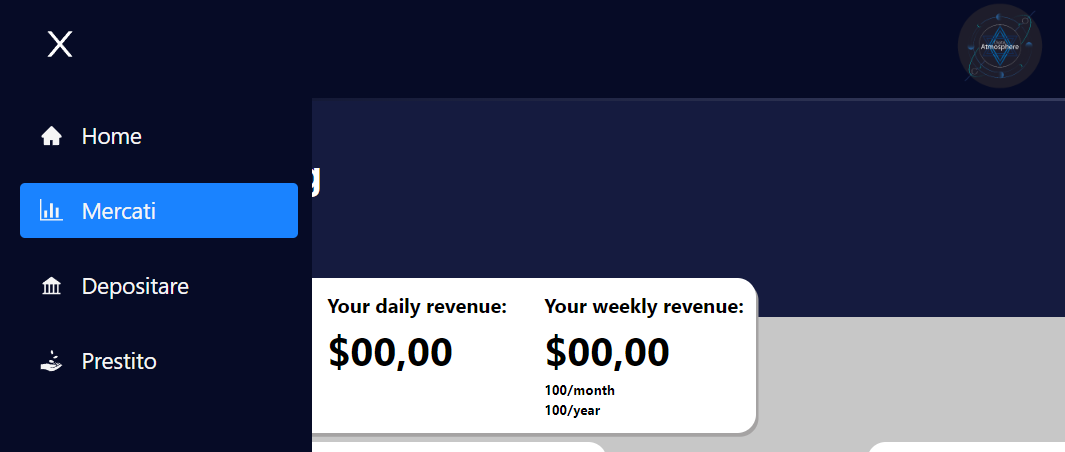
\includegraphics[width=13cm,height=6cm]{Immagini/sidebar.png}
    \caption[Sidebar dell'applicativo riferito allo staking]{Sidebar dell'applicativo.}
    \label{sidebar}
\end{figure}

Per quanto riguarda il Footer dell'applicazione, vengono mostrate piccole sezioni per le informazioni della compagnia, FAQ, supporto e icone per la renderizzazione ai rispettivi canali social. Viene mostrato in figura \ref{footer}.

\begin{figure}[h]
    \centering
    
\includegraphics[width=14cm,height=4cm]{Immagini/footer.png}
    \caption[Footer dell'applicativo riferito allo staking]{Footer dell'applicativo.}
    \label{footer}
\end{figure}

I due elementi appena mostrati vengono definiti nelle componenti \textcourier{Navbar.js} e \textcourier{Footer.js} con il relativo stile CSS importato al loro interno.

\subsubsection{Pagina principale}
La pagina principale dell'applicazione consiste in tanti Card che mostrano diverse informazioni all'utente. Queste informazioni devono essere prelevate, elaborate e mostrate in maniera adeguata al fruitore dei servizi dell'ipotetico applicativo finale che verrà sviluppato su questo prototipo.
Prima di presentare le interfacce dell'applicazione introdotta in (\ref{staking_app}), mostriamo la struttura delle componenti e della loro gerarchia in figura \ref{struttura_staking}.
\begin{figure}[h]
    \centering
    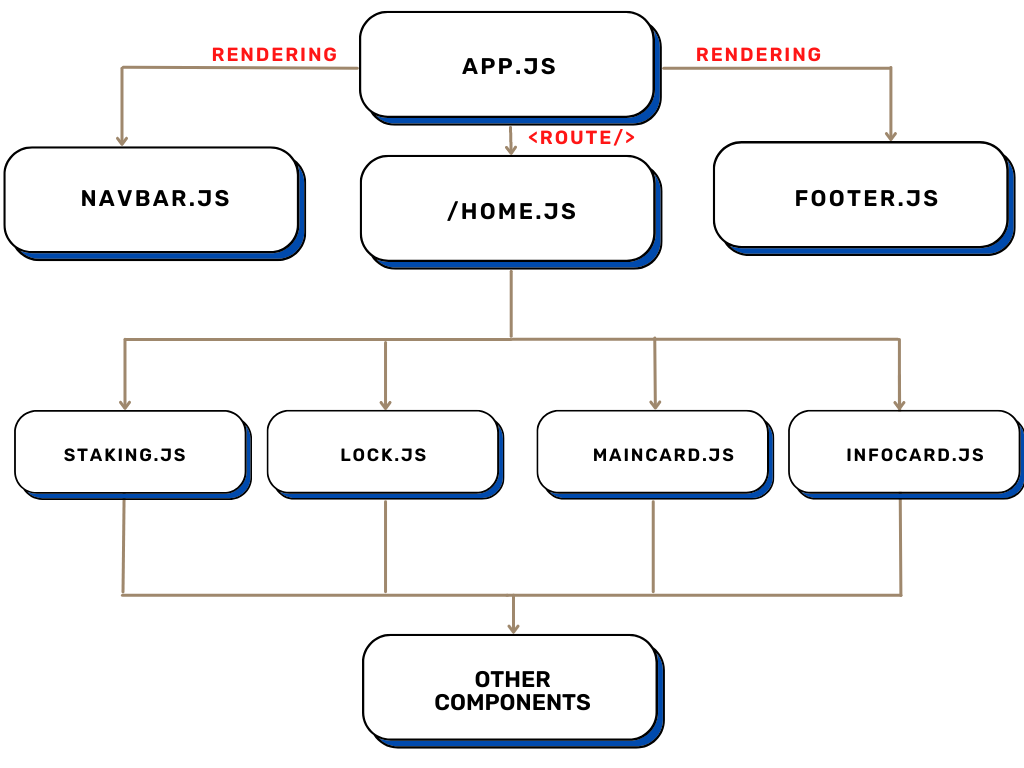
\includegraphics[width=14cm,height=8cm]{Immagini/StakingChart.png}
    \caption[Albero delle componenti dell'applicativo riferito allo staking]{Struttura delle componenti dell'applicativo riferito allo staking.}
    \label{struttura_staking}
\end{figure}
Alla radice della nostra applicazione, come di consuetudine per ogni applicazione in React, c'è \textcourier{App.js}, la quale è collegata (attraverso meccanismi interni approfonditi in \ref{Struttura_componenti}) alle componenti successive dell'albero. Al di sotto della radice (oltre alle componenti sempre presenti \textcourier{Navbar.js} e \textcourier{Footer.js}) c'è la rotta riferita ad \textcourier{Home.js} la quale possiede a sua volta altre 4 componenti principali in cui cono presenti i Card principali per la visualizzazione dei dati: \textcourier{InfoCard.js}, \textcourier{Staking.js}, \textcourier{Lock.js}, \textcourier{MainCard.js}.


I primi Card, mostrati in figura \ref{Card1}, fanno parte della componente \textcourier{MainCard.js}, comunicano all'utente la loro disponibilità dei token ATMOS (i quali vengono conteggiati attraverso Metamask), le revenue giornaliere, mensili e annuali, i relativi token depositati e messi in stake.
Le informazioni in questione possono essere mostrate soltanto agli utenti connessi all'applicazione. La logica della \ref{Connessione a Metamask} verrà mostrata nella parte dell'elaborato relativa all'implementazione dell'exchange. 

\begin{figure}[t]
    \centering
    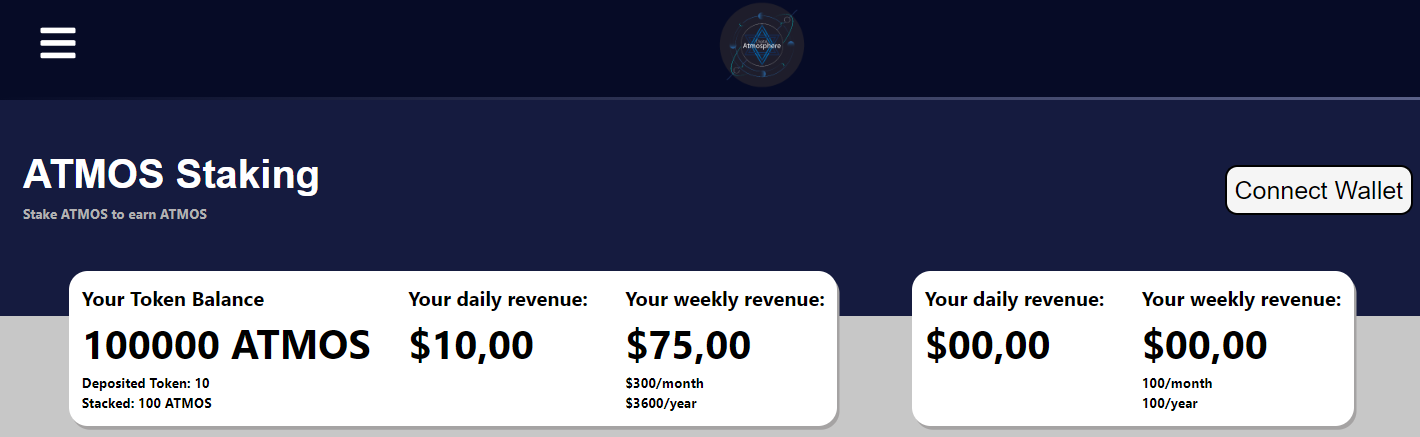
\includegraphics[width=14cm,height=4.5cm]{Immagini/Card1.png}
    \caption[Main Card per il balance e le revenue]{Card che mostrano il balance e le revenue dell'utente collegato.}
    \label{Card1}
\end{figure}
\begin{figure}[h]
    \centering
    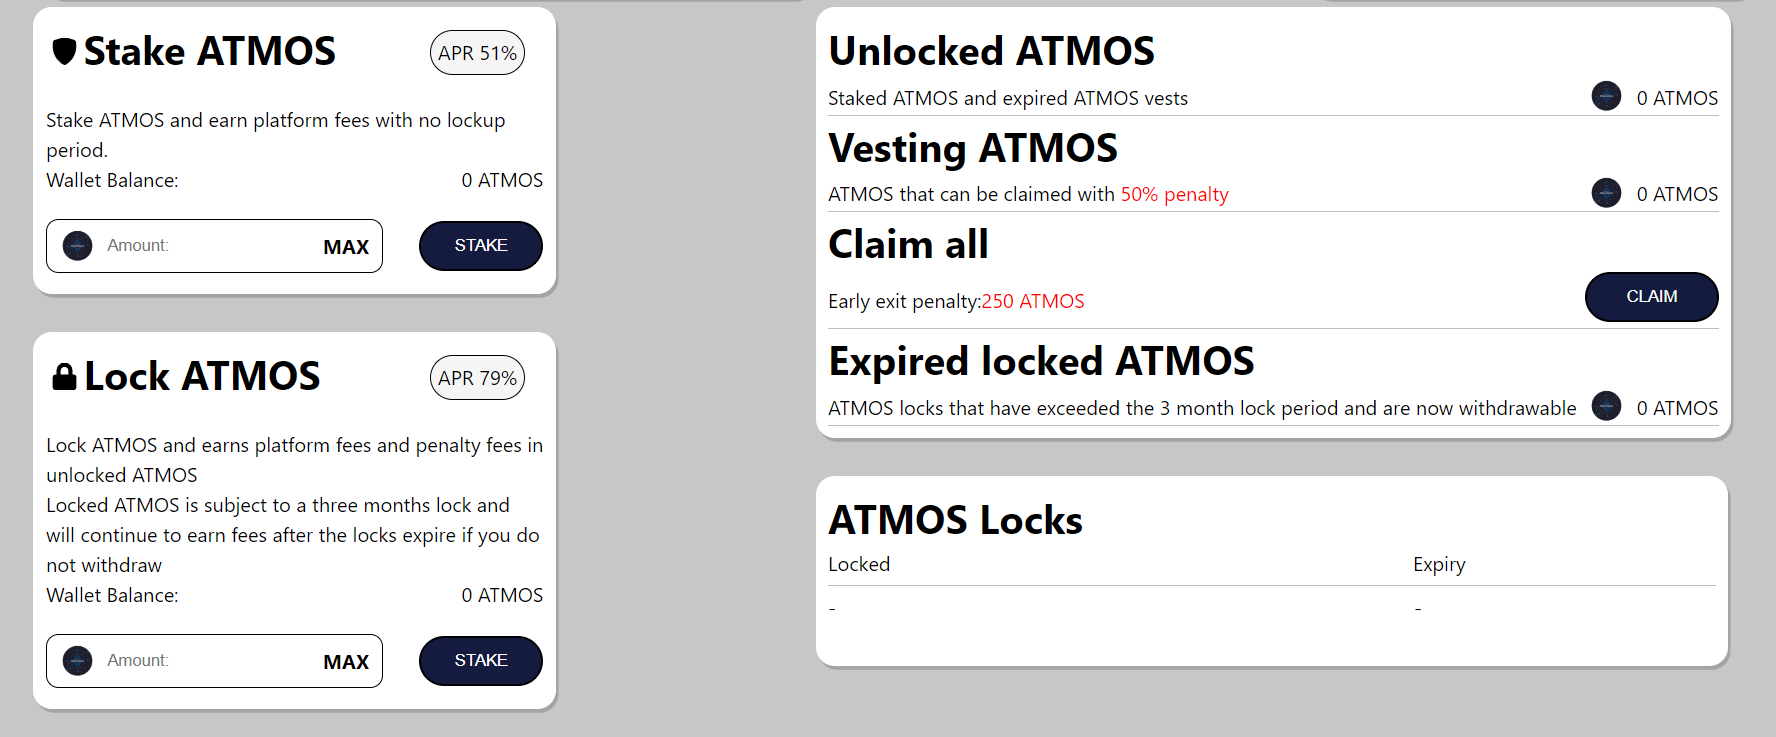
\includegraphics[width=12cm,height=5cm]{Immagini/Card2.png}
    \caption[Card con i form per la messa in stake e in lock dei token]{Card che mostrano i form per la messa in stake e in lock dei token.}
    \label{Card2}
\end{figure}
Invece, per quando riguarda il corpo vero e proprio dell'applicativo, i Card mostrati in figura \ref{Card2} cono composti da form per mettere in stake e in lock\footnote{Il lock di token si riferisce a un periodo di tempo specifico in cui i token non possono essere inoltrati o scambiati.Tipicamente, viene utilizzato come strategia preventiva per mantenere un valore stabile a lungo termine di un particolare asset.} quantitativi variabili di token ATMOS. Questi Card appartengono alle componenti \textcourier{Staking.js}, \textcourier{Lock.js} e \textcourier{InfoCard.js}, i quali, attraverso il codice JSX e il CSS specifico importato nelle componenti, renderizza gli elementi descritti.

Una volta inserito l'ammontare di token da mettere in stake o in lock, l'utente dovrà cliccare sul bottone riferito all'operazione corrispondente; si dovrà poi confermare l'operazione attraverso l'approvazione dei token che si vogliono utilizzare. Come è stato accennato in \ref{metamask}, Metamask gestisce tutte le comunicazioni con la Blockchain integrando la visualizzazione per la conferma di operazioni (come quella dell'approvazione nel nostro caso specifico) in pop-up che vengono visualizzati all'utente in maniera molto veloce e sintetica. Si mostra in figura \ref{approve} un esempio di chiamata all'approve dei nostri token ATMOS.



L'operazione di approvazione consiste nell'impostare un valore (nel nostro caso l'importo inserito nei form) come indennità di spesa sui token del chiamante. La funzione di approve appartiene all'ABI standard dei token ERC-20 e richiede come parametri il valore appena accennato e l'address del token ERC-20 per cui si vuole fare l'approvazione.  Con questa funzione, si può assegnare ad un altro indirizzo i permessi di spendere i token. La limitazione sui token che si approvano permette di evitare exploit o l’azzeramento dei fondi da parte di malintenzionati.
\begin{figure}[h]
    \centering
    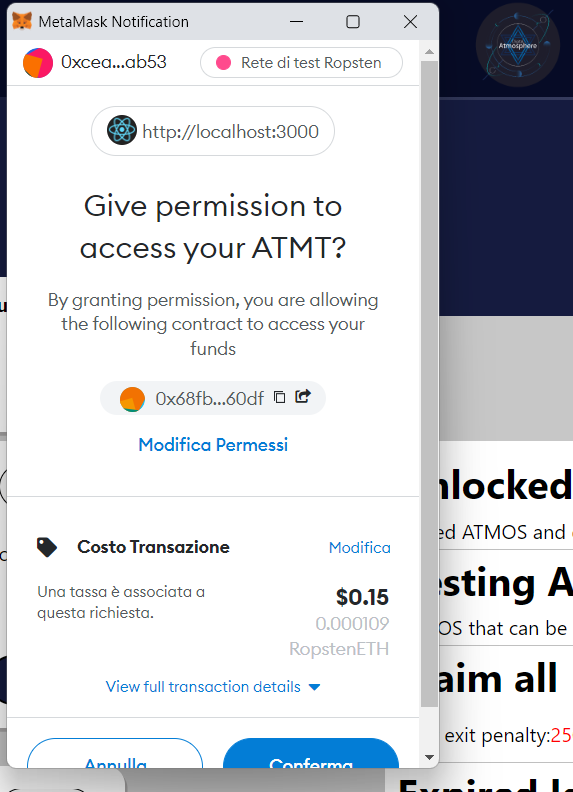
\includegraphics[width=4cm,height=6cm]{Immagini/approve.png}
    \caption[Schermata di approvazione dei token ATMOS]{Esempio di approvazione dei token ATMOS tramite Metamask.}
    \label{approve}
\end{figure}
Come anticipato, React utilizza il Virtual DOM per apportare modifiche o per effettuare controlli specifici; sfruttiamo questo vantaggio per controllare se l'utente possiede abbastanza token oppure se è stata effettuata l'approvazione prima di un'operazione. La visualizzazione del messaggio viene mostrata in figura \ref{controllo}.

\begin{figure}[h]
    \centering
    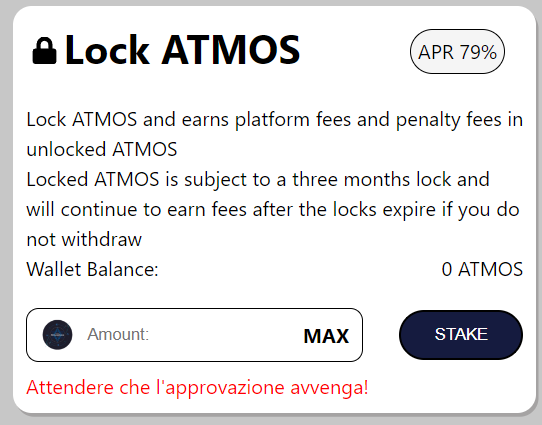
\includegraphics[width=10cm,height=8cm]{Immagini/Controllo.png}
    \caption[Schermata di warning per la mancata approvazione dei token]{Messaggio di mancata approvazione dei token visualizzato nel Card.}
    \label{controllo}
\end{figure}

Il controllo in questione deve essere fatto finché un ipotetica operazione \textit{asincrona}\footnote{Un'operazione asincrona è un'unità di lavoro che funziona separatamente dal thread principale, notificando, successivamente, quando avrà finito il lavoro.} (che sia un'approve oppure la richiesta della conferma di un'operazione attraverso Metamask) non venga terminata o confermata dall'utente. Così facendo, si simula l'handling dei messaggi di errore, così come si farebbe con JQuery\footnote{Libreria JavaScript progettata per semplificare l'attraversamento e la manipolazione dell'albero DOM HTML, nonché la gestione degli eventi, l'animazione CSS e Ajax.}. 

\section{Implementazione dell'exchange}\label{exchange}
La maggior parte del lavoro di questo elaborato è stato dedicato alla realizzazione di un exchange decentralizzato (DEX), anch'esso strutturato sulla rete di test Ropsten su Blockchain Ethereum.

Prima di indentrarci nell'implementazione, c'è bisogno di introdurre il funzionamento dei DEX e, quindi, di un Automatic Market Maker (AMM).
Verrà mostrato il motivo per il quale i DEX hanno rivoluzionato il mondo della finanza decentralizzata (DeFi), definendo tutte le logiche, le caratteristiche e i servizi da essi offerti.

\subsection{Exchange Decentralizzato (DEX)}\label{dex}
La finanza decentralizzata (DeFi) ha offerto al mondo un modo notevolmente migliore di fare trading e di guadagnare entrate passive, in questo caso tramite le criptovalute. Prima che esistesse la DeFi, il trading veniva condotto dagli \textit{exchange centralizzati} (CEX) , i quali vengono creati e organizzati da organizzazioni centralizzate che fungono da intermediari tra gli acquirenti e i venditori. Essi mantengono il controllo sulle chiavi private (evitando agli utenti l'onere di gestirle), i parametri di trading e le informazioni relative all'utente; memorizzano i dati di tutti gli ordini di acquisto e di vendita per un determinato asset che l'utente effettua, archiviandoli all'interno di un database centralizzato.
Il controllo e la gestione degli elementi appena citati, rende questi exchange molto facili da utilizzare, anche per utenti nuovi nel settore.

Uno dei più grandi svantaggi dei CEX è quello legato alla sicurezza: lasciare che l'exchange gestisca la chiave per il portafoglio significa che qualsiasi risorsa al suo interno non è veramente tua; di fatto se l'exchange venisse violato, o addirittura avvenisse un fallimento dell'azienda, tutto quello che si possiede nel proprio portafogli andrebbe perso. In poche parole, i CEX sono un compromesso per gli utenti che non vogliono avere l'onere, come anticipato, di gestire le proprie chiavi.

Un'\textit{exchange decentralizzato} (DEX), invece, si porta con sé le caratteristiche derivanti dalla DeFi, preservando l'etica crittografica e rendendolo uno strumento sicuro e privo di intermediazione.
Senza un'entità centrale non esisterà una piattaforme in cui depositare dei fondi, l'utente dovrà soltanto collegare il proprio portafoglio al DEX utilizzando le proprie chiavi private. Questo ovviamente implica l'onere di gestire con cura e con attenzione le proprie chiavi; d'altra parte, rende le risorse in tutto e per tutto controllabili solo dall'utente e non da entità centrali.

I DEX, inoltre, non interagiscono con il denaro fiat\footnote{Con denaro fiat si intende una valuta emessa dal governo che non è supportata da un bene fisico, come oro o argento, ma piuttosto dal governo che l'ha emessa.}, quindi non necessitano la conformità a KYC\footnote{acronimo di Know Your Customer (letteralmente: “conosci il tuo cliente”), è l’insieme di procedure che devono essere attuate da alcuni istituti e professionisti per obbligo di legge. Queste procedure servono per acquisire dati certi e informazioni sull’identità dei loro utenti e clienti.}.
Grazie a questo, la tua privacy, le tue informazioni personali e i tuoi dati sensibili non possono essere visti o hackerati da nessuna persona ( i dati non fanno parte di nessuna istituzione o ente centrale).
Esistono due differenti tipi di DEX:
\begin{itemize}
\item  Basato sugli \textit{Order-book}: i quali utilizzano un algoritmo (invece di una piattaforma centrale) per trovare e instradare gli scambi tra i singoli utenti. Gli smart-contract registrano gli scambi sulla Blockchain per riflettere gli asset che si spostano tra acquirenti e venditori. Non esiste un mercato vero e proprio, nel mezzo si interpone solo un algoritmo, rendendo comunque il servizio decentralizzato;
\item Gli \textit{Automatic Market Maker} (AMM): la nostra applicazione si posizione in questa categoria di DEX, nel paragrafo successivo (\ref{AMM}) si approfondisce il tema in questione.
\end{itemize}

\subsection{Automatic Market Maker (AMM)}\label{AMM}
Gli Automatic Market Maker (AMM) sono dei sistemi basati su Blockchain che permettono il trading \textit{automatizzato} attraverso scambi di criptovalute decentralizzati, il tutto regolato dagli smart-contract. In un contesto di questo tipo, il codice degli smart-contract è legge, il quale elabora tutte le transazioni automaticamente, senza fare affidamento su richieste di acquisto/vendita di terze parti per i token scambiati. Prenderemo in esempio il protocollo di Uniswap \cite{uniswap_docs} per la spiegazione tecnica del funzionamento di questi sistemi. 

\subsubsection{Pool di liquidità}\makeatletter\def\@currentlabel{Pool di liquidità}\makeatother\label{pool_liquidità}
Tra gli smart-contract più importanti di un AMM ci sono quelli riferiti al \textit{Pool di liquidità}.
Un\textit{ Pool di liquidità}, come mostrato nella rappresentazione \ref{pool} in \cite{uniswap_pool}

\begin{figure}[h]
    \centering
    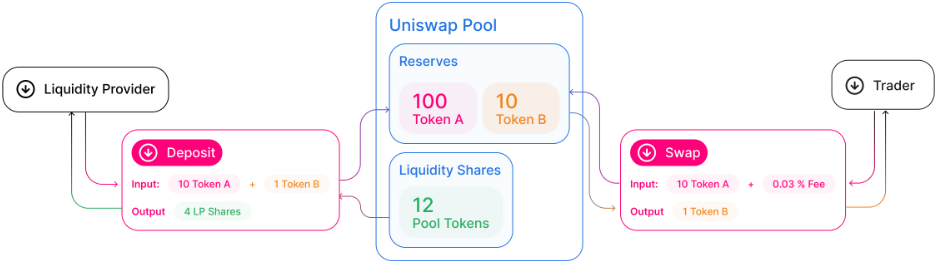
\includegraphics[width=13cm,height=4cm]{Immagini/Pool.png}
    \caption[Rappresentazione grafica di un Pool di Liquidità]{Rappresentazione grafica di un Pool di Liquidità.}
    \label{pool}
\end{figure}


non è altro che una raccolta di token crittografici, che viene utilizzato per rendere possibile il trading tramite un algoritmo che definisce i prezzi dei token in base al rapporto variabile dei token forniti; infatti, come definito in \cite{uniswap_pool}:“Ogni pool di liquidità è una sede di negoziazione per una coppia di token ERC-20.[...]”.

Ogni \textit{Pool di liquidità} è composto da due token (nel caso di Uniswap da due token ERC-20), ecco perché i pool di liquidità sono anche chiamati coppie (o Pair).
Quando viene creato un nuovo contratto Pool i saldi di ciascun token sono uguali a zero, saranno i Liquidity Provider (LP, letteralmente fornitori di liquidità) o market maker, che forniranno la liquidità ai pool sotto forma di asset digitali. I primi fornitori del pool saranno anche coloro che determineranno il prezzo iniziale del Pool. I Liquidity Provider (LP) fanno parte della prima parte, raffigurata in figura \ref{liquidity}.
\begin{figure}[h]
    \centering
    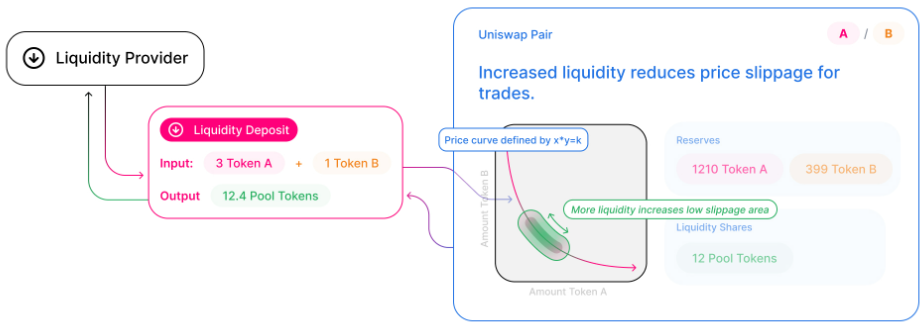
\includegraphics[width=12cm,height=4cm]{Immagini/liquidity.png}
    \caption[Rappresentazione grafica del funzionamento per il deposito liquidità da parte dei Liquidity Provider (LP)]{Rappresentazione deposito liquidità da parte dei Liquidity Provider (LP).}
    \label{liquidity}
\end{figure}

Negli AMM, è importante notare come i Pool con grandi quantità di trade attivi (e quindi grande liquidità) prosperino sulla rete, mentre i Pool con bassa liquidità causano enormi impatti sui prezzi e slittamenti vari, rendendoli, quindi, inefficaci. Inoltre, per depositare fondi in un pool, è necessario fornire una stessa quantità di liquidità per token.

Questi vincoli nascono affinché tutti gli utenti possano scambiare qualsiasi token in qualsiasi momento; il Pool deve sempre disporre di quantità sufficienti di entrambi i token della coppia del Pool, pertanto, ogni DEX che opera sul modello AMM è interessato ad avere una liquidità più grande possibile. Per ottenere una grande liquidità nei Pool, ogni AMM incentiva gli utenti a depositare token nei propri Pool, tramite il concetto di \textit{yield farming}( o liquidity mining).

L'idea dello \textit{yield farming} è quella di ricompensare gli utenti fornitori di liquidità con delle commissioni speciali, chiamate \textit{commissioni LP}(o LP token), ossia commissioni di negoziazione distribuite in maniera proporzionale alla quantità di liquidità apportata, rappresentante una parte di proprietà del Pool. Se un Liquidity Provider (LP) vuole rimuovere liquidità e riacquisire i propri asset, deve bruciare i suoi LP token per recuperare gli asset ( ossia i token originali).

\subsubsection{Token Swaps}
Dall'altra parte dell'AMM, come mostrato in figura \ref{swap}, c'è la sezione relativa ai Trader.
\begin{figure}[h]
    \centering
    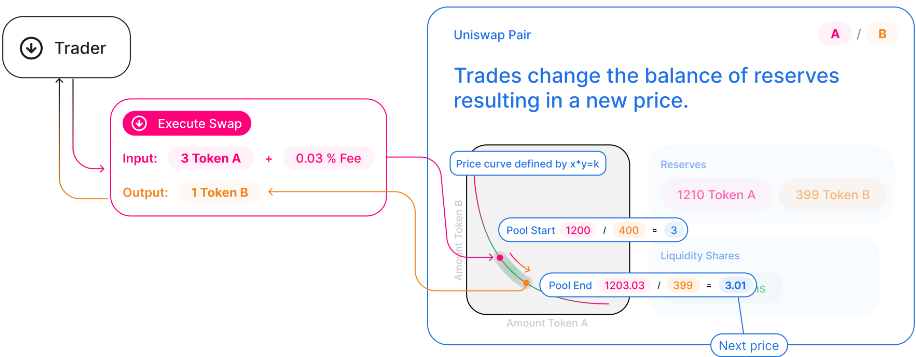
\includegraphics[width=12cm,height=4cm]{Immagini/Swap.png}
    \caption[Rappresentazione grafica del funzionamento relatico al trading di token]{Sezione relativa al trading di token.}
    \label{swap}
\end{figure}
I trader rappresentano tutti quegli utenti che desiderano scambiare token per altri token e pagare il prezzo in base alla riserva di liquidità (mostrata in figura \ref{pool}) nel contratto.
Come anticipato in (\ref{pool_liquidità}), ogni coppia di token è supportata da un Pool di liquidità, il quale, ricordiamo, non è altro che uno smart-contract che definisce tutte le operazione per quanto riguarda le operazioni di deposito e di prelievo, oltre che utilizzato per detenere i saldi dei due token. Per assicurarsi che il rapporto tra le attività nei pool di liquidità rimanga il più equilibrato possibile eliminando eventuali discrepanze nei prezzi delle attività nei pool, gli AMM utilizzano equazioni matematiche preimpostate. Nel caso di Uniswap, come definito in \cite{uniswap_swap}, viene utilizzata la “\textit{formula del prodotto costante}” ossia:
\begin{equation*}
		x \cdot y=k ,dove:
\end{equation*}\begin{itemize}
\item \textit{x} rappresenta il valore del primo asset (token A);
\item \textit{y} rappresenta il valore del secondo asset (token B);
\item \textit{k}, invece, è una costante.
\end{itemize}

Sostanzialmente Uniswap, attraverso questa formula, mantiene sempre un valore costante, uguale nel tempo, per la moltiplicazione del prezzo del token A col token B. Prendiamo in esempio un ipotetico Pool di liquidità tra un token A e un token B: se il token A viene acquistato dai trader, il token B verrà aggiunto al Pool, rimuovendo il token A da esso. Questa operazione fa diminuire la quantità del token A all'interno del Pool, il che, a sua volta, fa aumentare il suo prezzo (proprio per soddisfare l'effetto di bilanciamento della formula sopra citata). Mentre il prezzo del token A aumenta di prezzo, il prezzo del token B diminuisce a sua volta perché aggiunto al Pool.

\subsubsection{Routing }\makeatletter\def\@currentlabel{Routing}\makeatother
\label{Routing}
Spesse volte i trader hanno bisogno di scambiare tipologie di asset per i quali non esiste un Pool di liquidità; la creazione di un Pool potrebbe essere molto costoso per alcuni trader, di conseguenza, per far fronte a questo problema, è nato il concetto del \textit{Routing}.
Il \textit{Routing} è quella procedura che permette ai trader (o utenti della Dapp fruitori dei servizi) di scambiare asset anche quando non esiste un Pool di liquidità tra una coppia di asset su cui vogliono operare.
Questa procedura consiste nello scandagliare tutti i Pool di liquidità che esistono tra i due token della coppia che si vuole scambiare e scegliere la \textit{Custom Path} (la rotta) da seguire per ottenere il miglior prezzo possibile per l'acquirente. Lo smart-contract che si occupa di effettuare l'operazione di Routing è il \textit{Router Contract} (che approfondiremo nei paragrafi successivi). Il contratto in questione, esegue queste operazioni totalmente in background, in un unica transazione di scambio, in maniera tale che l'utente non si accorga di nulla e renda le operazioni molto più semplificate. Un esempio di rotta tra Pool di liquidità viene mostrato nella figura \ref{routing}.

\begin{figure}[h]
    \centering
    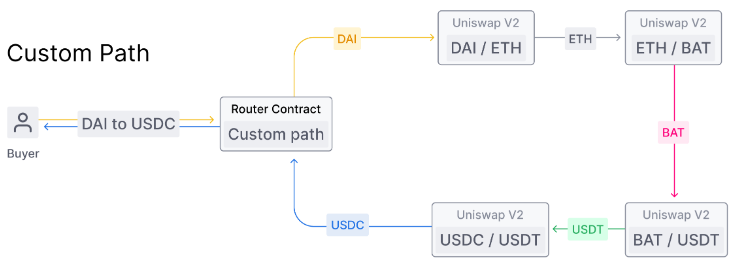
\includegraphics[width=13cm,height=5cm]{Immagini/Routing.png}
    \caption[Custom Path per il Routing tra pool di liquidità]{Esempio di Routing tra più Pool di liquidità.}
    \label{routing}
\end{figure}

\subsection{Interfaccia Grafica dell'applicativo}\label{UI_dex}
La maggior parte del lavoro correlato a questo elaborato consiste, come già anticipato, nell'implementazione di un exchange decentralizzato (DEX) distribuito sulla rete di test Ropsten di Ethereum. L'applicativo in questione consta di due pagine principali:
\begin{itemize}
\item La pagina relativa allo \textit{Swap} dei token ERC-20 presenti sulla rete di Ethereum;
\item La pagina relativa ai \textit{Pool di liquidità} per ogni coppia di token su cui si vuole operare.
\end{itemize}

Queste due pagine rappresentano le parti nelle quali si concentra tutta la logica dell'exchange e l'interazione vera e propria con gli smart-conctract sviluppati in Solidity (approfondiremo la logica in \ref{interazione_smartc}).
Mostriamo ora l'interfaccia grafica dell'applicativo, la quale è stata pensata per essere user-friendly, facile da utilizzare e intuitiva il più possibile.

\subsubsection{Struttura delle componenti}\label{Struttura_componenti}

Prima di mostrare le varie interfacce implementate, definiamo la struttura delle componenti che abbiamo scelto per la nostra applicazione React. Si è sintetizzata la gerarchia delle componenti nella figura \ref{struttura_componenti}.
\begin{figure}[h]
    \centering
    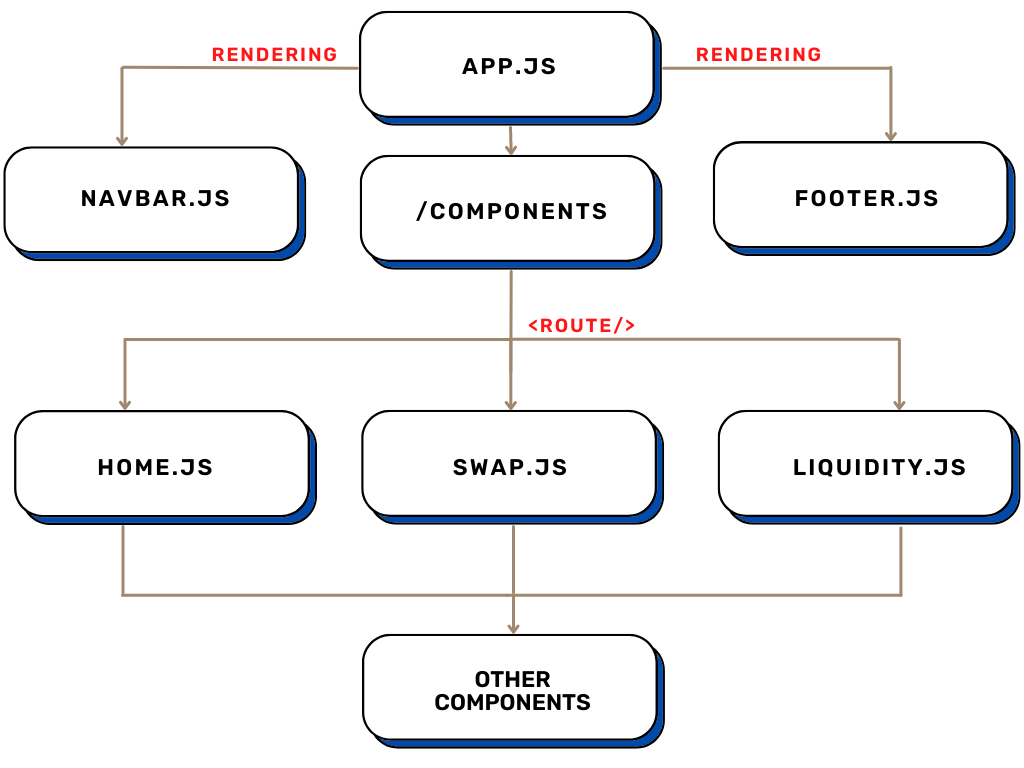
\includegraphics[width=14cm,height=8cm]{Immagini/StrutturaComponenti.png}
    \caption[Albero delle componenti dell'applicativo riferito all'exchange]{Struttura delle componenti dell'applicativo riferito al DEX.}
    \label{struttura_componenti}
\end{figure}
\\Come si può notare, alla radice della nostra gerarchia c'è la componente \textcourier{App.js}, la quale esegue il rendering dell'interfaccia utente globale dell'app e configura tutte le \textit{variabili di stato} necessarie al corretto funzionamento delle procedure eseguite nelle altre componenti renderizzate da quest'ultima. Per il corretto rendering delle componenti sottostanti ad \textcourier{App.js} si utilizza la libreria \textcourier{react-router}, in quanto un'app React di base non consente l'instradamento delle pagine. Una volta scaricata la libreria tramite il comando \textcourier{npm install react-router --save}, è possibile definire diverse “rotte” per la nostra applicazione (come mostrato in figura \ref{struttura_componenti}).
Di seguito si mostra il codice JSX del rendering delle componenti principali della gerarchia (notare come queste siano solo le principali, ogni componente possiede altre sotto-componenti per la gestione dinamica delle proprie funzionalità specifiche):\\


\begin{lstlisting}[caption={[App.js (exchange)]},language=jsx] 
return (
 <>
   <Router>
   
   {/*Navbar component*/}
   <Navbar isConnected={isConnected}
   currentAccount={currentAccount}
   web3={web3} showCard={showCard} 
   active={active}/>
   
 {/*ROTTE DELLA PIATTAFORMA*/}
 <Switch>
 
		<Route path='/swap'
        render={()=> <Swap web3={web3} 
        router={routerContract} factory={factoryContract}  
        isConnected={isConnected} showCard={showCard}
        currentAccount={currentAccount}/>}
        />

    <Route path='/liquidity'
        render={()=> <Liquidity web3={web3} 
        router={routerContract} factory={factoryContract}  
        isConnected={isConnected} showCard={showCard}
        currentAccount={currentAccount}/>}
        />
         
 </Switch>

   {/*Footer component*/}
   <Footer/>

   </Router>
</>
);																												-App.js
\end{lstlisting}\makeatletter\def\@currentlabel{App.js}\makeatother
\label{App.js}

Come è visibile nel codice JSX di \ref{App.js}, le componenti \textcourier{Navbar.js} e \textcourier{Footer.js} sono sempre presenti, a prescindere dalla rotta, per ogni rendering della pagina.
Questo perché la Navbar e il Footer, in generale in un'applicazione web, sono due elementi essenziali che, solitamente, si ripetono in ogni pagina.
Nella riga 19 e 26 ,rispettivamente, vengono definite le rotte per le componenti principali dell'applicazione sviluppata:
\begin{itemize}
\item La componente \textcourier{Swap.js} la quale interfaccia sarà approfondita in (\ref{Swap.js});
\item La componente \textcourier{Liquidity.js} la quale interfaccia sarà approfondita in (\ref{Liquidity.js}).
\end{itemize}
Prima di approfondire le due componenti sopra citate, nel paragrafo successivo verrà spiegato come avviene la connessione al nostro wallet digitale (e quindi la possibilità di comunicare in maniera molto semplificata con la Blockchain), le funzioni chiamate attraverso la libreria \textit{web3.js} e le relative interfacce grafiche per l'autenticazione.
\subsubsection{Connessione a Metamask }\makeatletter\def\@currentlabel{Connessione a Metamask}\makeatother
\label{Connessione a Metamask}

La connessione al wallet di Metamask (e il relativo accesso ai propri token), viene gestita tramite la libreria \textit{web3.js}; a livello grafico, viene mostrato un bottone all'interno della Navbar \ref{navbar}, il quale, all'\textit{onClick}, tramite delle funzioni CSS, rende il background sfocato per dirigere l'attenzione dell'utente su un Card (renderizzato dalla componente \textcourier{ConnectionCard.js}) che visualizza graficamente diversi provider ai quali ci si può collegare. Nel nostro caso prenderemo in esempio l'utilizzo di Metamask.

\begin{figure}[h]
    \centering
    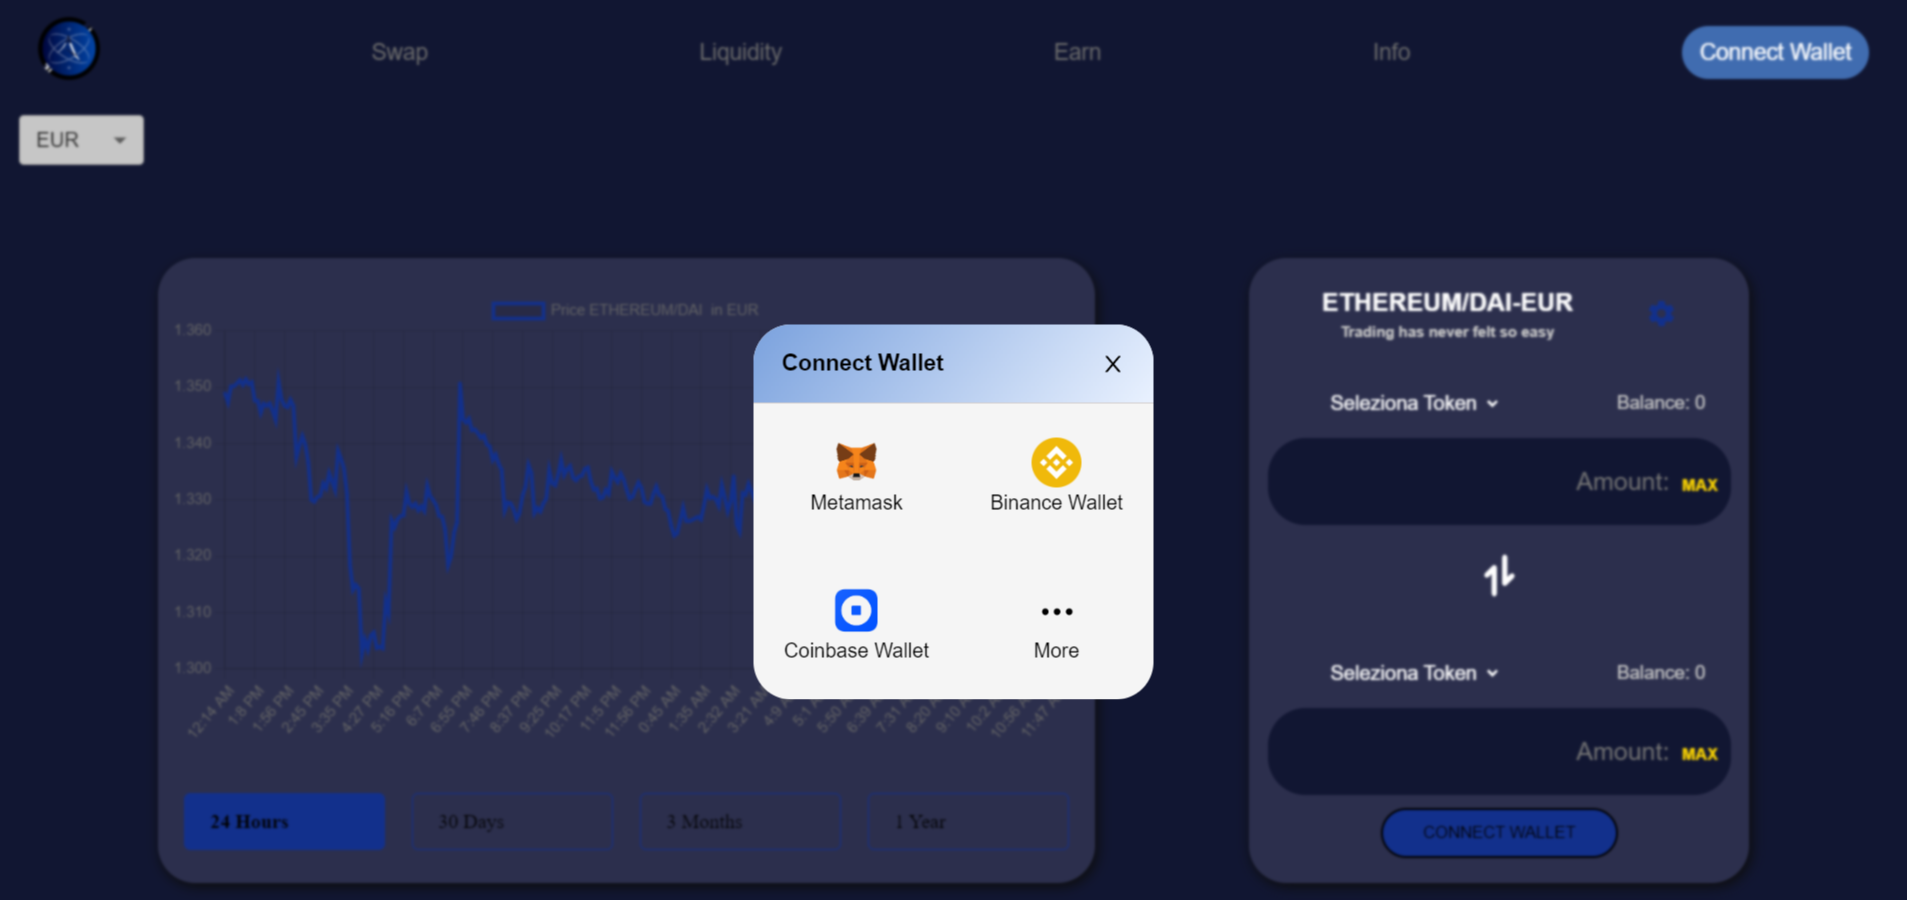
\includegraphics[width=15cm,height=7cm]{Immagini/navbar.png}
    \caption[Scelta provider per la connessione alla Dapp]{Card per la scelta del provider visualizzato all'\textit{onClcik} del bottone “Connect Wallet”.}
    \label{navbar}
\end{figure}

Una volta scelto il wallet, viene eseguita la funzione \ref{onLogin}: il codice viene mostrato di seguito.
\begin{lstlisting}[caption={[\textcourier{onLogin()} Function]},language=jsx] 
const onLogin = async (provider) => {
        const web3= new Web3(provider)
        const accounts = await web3.eth.getAccounts();
        const chainId = await web3.eth.getChainId();
        if (accounts.length === 0) {
            console.log("Please connect to MetaMask!");
        } else if (accounts[0] !== currentAccount) {
        setProvider(provider);
        setWeb3(web3);
        setCurrentNetwork(chainId);
        setCurrentAccount(accounts[0]);
        setIsConnected(true);
        window.localStorage.setItem('IS_CONNECTED',accounts[0]);

        /*Create local contracts copy */
        const factory=SetAtmosFactoryContract(web3)
        setFactoryContract(factory)

        const router=SetAtmosRouterContract(web3)
        setRouterContract(router)
        }
    };        																			     -onLogin
\end{lstlisting}\makeatletter\def\@currentlabel{onLogin}\makeatother
\label{onLogin}

Nella funzione \textcourier{\ref{onLogin}\textcolor{red}{()}}, viene utilizzata una funzione del pacchetto \\\textcourier{web3.eth}: la funzione \textcourier{getAccounts()}, che non fa altro che restituire l'elenco degli account controllati dal nodo, come definito in \cite{web3API}. Nella riga 3 viene assegnato l'oggetto restituito dalla funzione; se questo oggetto esiste significa che l'utente ha effettuato con successo la connessione a Metamask, altrimenti si controlla (nella riga 7) se l'account con il quale si è fatto l'accesso è diverso dall'account corrente: in poche parole si verifica se un utente ha già effettuato l'accesso alla Dapp. Se sì, la funzione termina la sua esecuzione perché i dati per quell'utente sono già stati settati, se no, invece, viene confermato che è il primo accesso dell'utente in questione e si settano tutte le variabili utili per il corretto funzionamento delle funzionalità successive. 
Da notare come le variabili vengono settate attraverso lo \textit{UseState Hook} di React, definito in \cite{React}. 
La schermata di caricamento col relativo inserimento della propria password, viene visualizzata finché non si completa la riga 3 della funzione \textcourier{\ref{onLogin}\textcolor{red}{()}} ( il comando \textcourier{await} viene utilizzato per attendere una \textit{Promise}\footnote{L'oggetto Promise rappresenta l'eventuale completamento (o fallimento) di un'operazione asincrona e il suo valore risultante.} e ottenere il suo valore), la quale attiva l'estensione Metamask del browser web, mostrando un pop-up con un form per l'inserimento dei dati relativi all'accesso. Viene mostrata la schermata nella figura \ref{caricamento_login}.

\begin{figure}[h]
    \centering
    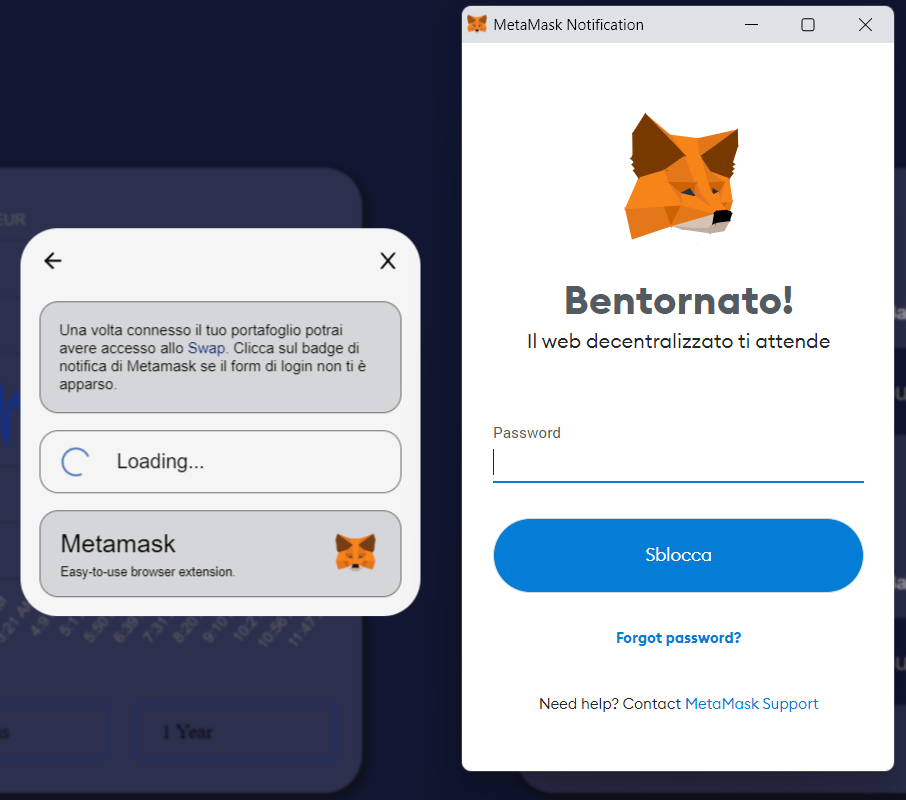
\includegraphics[width=13.5cm,height=10cm]{Immagini/VisualizzazioneMetamask.png}
    \caption[Schermata di caricamento per l'inserimento dei dati di accesso]{Schermata di caricamento in attesa che l'utente inserisca i dati di accesso.}
    \label{caricamento_login}
\end{figure}
Una volta effettuato l'accesso a Metamask, si visualizza l'indirizzo pubblico del proprio wallet direttamente nella Navbar dell'applicazione, in maniera tale da rendere la gestione dei propri address più semplice e intuitiva.

\subsubsection{Componente Swap.js}\makeatletter\def\@currentlabel{Swap.js}\makeatother\label{Swap.js}
La componente \textcourier{Swap.js} è la parte del nostro exchange che si occupa dello Swap dei token ERC-20 della rete Ethereum. L'interfaccia grafica della componente è composta da un grafico animato, strutturato grazie all'ausilio di una libreria React per la composizione di grafici: la libreria \textcourier{react-chartjs-2}, installata tramite il comando \textcourier{npm install react-chartjs-2}. Il grafico in questione si tratta di un \textit{Line Chart}, il quale riceve dei dati in input da parte di una API di \textit{CoinGecko} \cite{CoinGecko} che ottiene i dati storici (nome, prezzo, mercato, statistiche) in una determinata data per il singolo token. Il codice relativo alla chiamata dell'API viene mostrato in \ref{APIcode}. La chiamata all'API in questione è stata riscritta come una \textit{arrow function}\footnote{Scrittura alternativa (più pulita) di una funzione tradizionale. Questa funzionalità è stata introdotta nella versione ES6 di JavaScript.} rinominata “\textit{HistoricalChart}” nella componente \textcourier{API.js}. Questa funzione richiede tre parametri in input, rispettivamente: 
\begin{itemize}
\item L'id del token (ossia il nome del token) scelto per cui si vuole visualizzare il prezzo nel corso del tempo;
\item I days (giorni), ossia il range di tempo per ricevere l'istantanea dei dati;
\item La currency, ossia la valuta con cui si vuole visualizzare i prezzi (nell'applicazione vengono gestiti i prezzi in Euro e in Dollari).
\end{itemize}
Da notare come nella funzione \textit{HistoricalChart} siano stati utilizzati i \textit{Template Literals}, i quali permettono di creare stringhe interpolate, ossia stringhe con l'aggiunta dinamica di elementi all'interno di esse. 
\begin{lstlisting}[caption={[API Code]},language=jsx] 

  /*Componente API.js, la quale definisce tutte le chiamate API
  che si vogliono utilizzare per inviarle al server web*/
  
export const HistoricalChart = (id, days = 365, currency) =>
    `https://api.coingecko.com/api/v3/coins/${id}/market_chart?vs_currency=${currency}&days=${days}`;

  /*Componente Swap.js, parte relativa alla chiamata dell'API*/
  
import {HistoricalChart} from "../config/API";  
const fetchHistoricData = async () => {
        const dataTokenA = (await axios.get
        (HistoricalChart(tokenA ? tokenA.id : "ethereum", days, currency))).data;
        setHistoricDataTokenA(dataTokenA.prices);
    };

    useEffect(() => {
        fetchHistoricData();
    }, [days, tokenA, tokenB, currency])
    																							       -APIcode
\end{lstlisting}\makeatletter\def\@currentlabel{APIcode}\makeatother
\label{APIcode}
Per quanto riguarda, invece, la chiamata GET effettiva da mandare al server, si sfrutta un'altra libreria Javascript che ci permette di gestire le richieste effettuate tramite il protocollo HTTP e di connetterci alle API: la libreria \textcourier{axios}, installabile tramite il comando \textcourier{npm i axios} (la chiamata axios viene definita nella riga 12 di \ref{APIcode}).
Sempre in \ref{APIcode}, alla riga 17, viene utilizzato un'altro hook molto importante di React chiamato \textit{useEffect}, il quale, come si dice in \cite{React} :“consente di eseguire effetti collaterali nei componenti”; nel nostro caso, viene utilizzato per chiamare la funzione \textcourier{fetchHistoricData()} ogni volta che gli elementi presenti nelle \textit{dependency}\footnote{Un array di dipendenze richiesto facoltativamente dallo useEffect. L'hook esegue il suo contenuto solo se le dipendenze sono cambiate tra i rendering.} dell' hook vengono modificati. Questo meccanismo ci permette di rendere l'interfaccia utente molto dinamica, facendo sì che il grafico (in questo caso specifico) venga aggiornato ad ogni azione dell'utente, permettendogli una veloce e intuitiva comunicazione con l'applicazione. Viene mostrata in figura \ref{grafico} l'implementazione del grafico appena citato.

\begin{figure}[h]
    \centering
    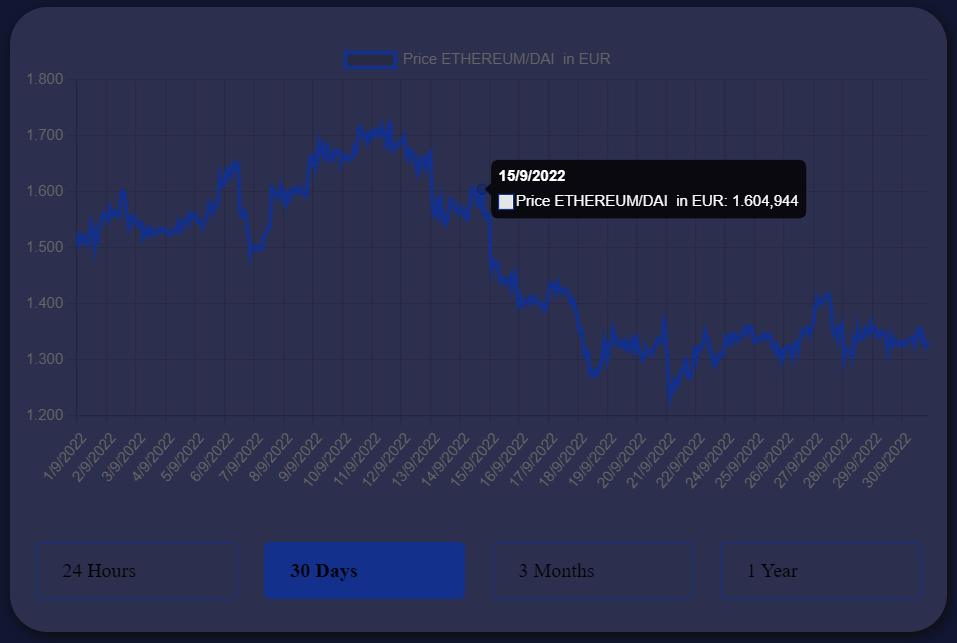
\includegraphics[width=13cm,height=8cm]{Immagini/Grafico.png}
    \caption[Line Chart implementato nell'applicativo riferito all'exchange]{Line Chart di esempio della coppia Ethereum/Dai-token.}
    \label{grafico}
\end{figure}
Come è possibile notare, il \textit{Line Chart} è una sorta di griglia sulla quale è tracciata una linea colorata che definisce l'andamento del prezzo nel corso del tempo. Il grafico possiede due serie di label: nella parte inferiore e nella parte laterale; nella parte laterale vengono definite le righe corrispondenti al prezzo della coppia tokenA/tokenB, mentre, nella parte inferiore, vengono tracciate le colonne, ognuna delle quali, corrisponde ad un determinato giorno. A seconda del bottone cliccato tra i quattro selezionabili nella parte sottostante, il grafico cambia forma in maniera del tutto animata, definendo una nuova traccia. Inoltre, se si passa col mouse su un punto del grafico è possibile visualizzare il prezzo in quella determinata data ( o orario).

La coppia di token mostrata nel grafico viene scelta attraverso il Card implementato per l'operazione di swap vera e propria. Il Card in questione (mostrato in figura \ref{swapCard}) ci permette di selezionare la coppia di token attraverso un \textit{dropdwon menu} di monete( o token) che si apre facendo click sull'etichetta “Seleziona Token”. Verrà inoltre mostrato il \textit{balance} (saldo) dello specifico token scelto andando a controllare le disponibilità nel wallet dell'account collegato alla nostra Dapp; questa procedura di verifica del balance viene effettuata attraverso il comando: 
\begin{quote}
\textcourier{ \textcolor{orangeWords}{await} tokenContract.\textcolor{purpleWords}{methods}.\textcolor{yellowFunction}{balanceOf}(props.\textcolor{purpleWords}{currentAccount}).\textcolor{yellowFunction}{call}()} 
\end{quote}\label{tokenContract}

dove \textit{tokenContract} è l'istanza di un oggetto \textcourier{web3.eth.Contract} rappresentate il token che è stato selezionato(approfondiremo l'interazione coi contratti dei token ERC-20 in \ref{interazione_smartc}), \textit{balanceOf} è un metodo definito nell'ABI del contratto di un token ERC-20 che richiede come unico parametro l'address del possessore di questi token (nel nostro caso abbiamo inserito il \textit{currentAccount}, ossia l'address dell'account connesso al momento).



\begin{figure}[h]
    \centering
    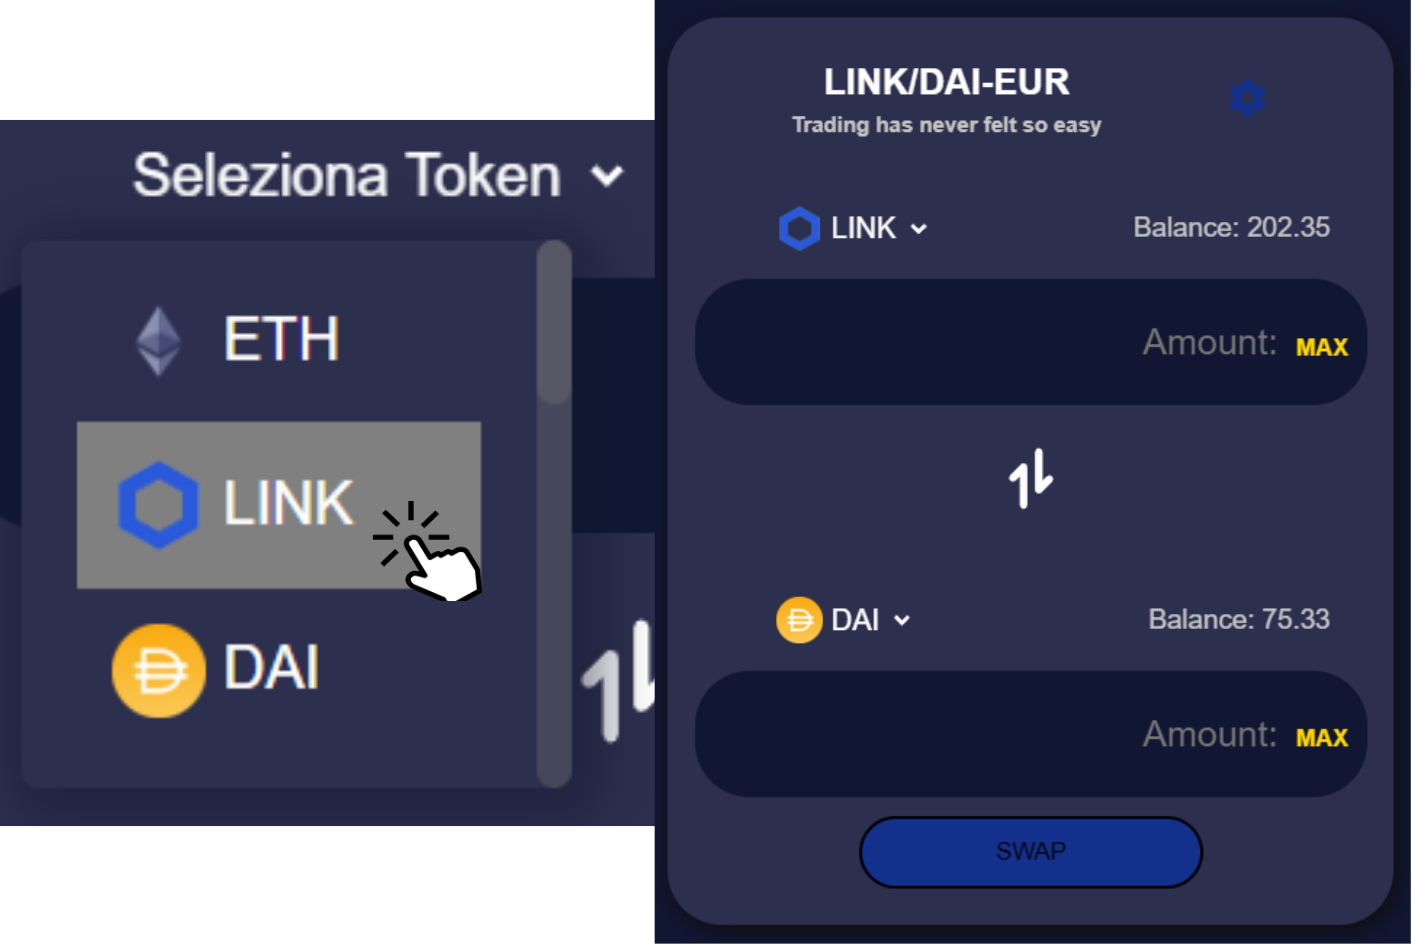
\includegraphics[width=12cm,height=8cm]{Immagini/SwapCard.png}
    \caption[Selezione dei token per il Card relativo allo Swap]{Selezione token per il Card relativo allo Swap.}
    \label{swapCard}
\end{figure}
Dal momento che l'EVM non supporta i numeri decimali, bisogna gestire il formato numerico con il quale, il dato token, è stato specificato alla sua creazione. Il formato è verificabile tramite la funzione \textcourier{decimals()} per ogni token ERC-20. 
Esistono token con differenti formati, di conseguenza, dal front-end bisogna gestire questa differenziazione per rendere leggibile i dati all'utente; nella nostra applicazione gestiremo i token con unità decimali più diffuse (dai 6 ai più famosi 18 decimals), di seguito viene mostrato il codice per la gestione delle conversioni (\ref{TokenConversion}).

\begin{lstlisting}[caption={[Token Conversion Code]},language=jsx] 
/*Import dell'ABI standard di un token ERC-20*/
import ERC20abi from "contracts/ERC20abi.json"
  const setTokenAContract = async (token) => {
        if(token.address != null) {
            const tokenContract = 
            new web3.eth.Contract(ERC20abi, token.address)
            const val = 
            await tokenContract.methods.balanceOf(props.currentAccount).call()
            if (token.decimals === 18) {  /*18 decimals token*/
                const bal=web3.utils.fromWei(val, "ether")
                setBalance(bal)
            }
            if (token.decimals === 8) {   /*8 decimals token*/
                const bal=web3.utils.fromWei(val, "gwei")
                setBalance(bal)
            }
            if (token.decimals === 6) {   /*6 decimals token*/
                const bal=web3.utils.fromWei(val, "mwei")
                setBalance(bal)
            }
        } else{  /*Se e' stato selezionato Ethereum nel menu*/
            const val=
            await web3.eth.getBalance(props.currentAccount)
            const bal=web3.utils.fromWei(val, "ether")
            setBalance(bal)
        }
    }
    																			       -TokenConversion
\end{lstlisting}\makeatletter\def\@currentlabel{TokenConversion}\makeatother
\label{TokenConversion}

Per la leggibilità dei dati all'utente, utilizziamo il pacchetto \textcourier{web3.utils} e la funzione \textcourier{web3.utils.fromWei()}, la quale richiede come parametri un valore (nel nostro caso il balance del token restituito dalla funzione \textcourier{balanceOf()} a riga 8) e una stringa che definisce in quale formato trasformare questo valore (la stringa deve essere scelta seguendo un \textit{unitMap} riportato in documentazione \cite{web3API}). Verrà mostrato su schermo il valore “balance” settato tramite useState nella funzione setTokenContract in \ref{TokenConversion}. 

Nel caso in cui venga selezionato Ethereum dal menu (il quale non è un token dello standard ERC-20 e non presenta un address specifico), il balance da mostrare riferito agli Ether disponibili nel wallet viene gestito dalla funzione a riga 22.  La funzione in questione fa parte del pacchetto \textcourier{web3.eth} e richiede come singolo parametro l'address dell'account da cui ottenere il dato; nel nostro caso è stato inserito l'account attualmente collegato all'applicazione. 

Come si può notare in figura \ref{swapCard}, il Card è composto, inoltre, da due form di input in cui è possibile selezionare il quantitativo di token che si vuole scambiare; una volta inseriti è possibile lanciare la chiamata allo smart-contract e alla relativa funzione per lo swap tramite il bottone con label “Swap”, la quale logica approfondiremo in \ref{interazione_smartc}.

Infine, si mostra la schermata generale comprensiva dei due Card appena descritti. La pagina mostrata in figura \ref{schermataSwap} riproduce la componente 
\textcourier{Swap.js} con il suo path specifico settato nell'URL dell'applicazione. Come si evince dalla figura, il grafico visualizza la traccia esatta per i token selezionati dal Card riferito all'operazione di swap (nel nostro esempio LINK e DAI); è presente, inoltre, un bottoncino in alto a sinistra per cambiare la \textit{currency} che l'utente desidera visualizzare nel grafico, il quale funzionamento è stato gestito tramite il meccanismo dei \textit{Context}, che, in poche parole, ci permette di condividere dati considerati “globali” per un albero di componenti in React. Questo meccanismo può tornare utile per definire funzioni o variabili richiesti da molte componenti; siccome il cambio della valuta è un elemento prioritario in un exchange, si è pensato di gestire il “cambio” in questa maniera.

\begin{figure}[h]
    \centering
    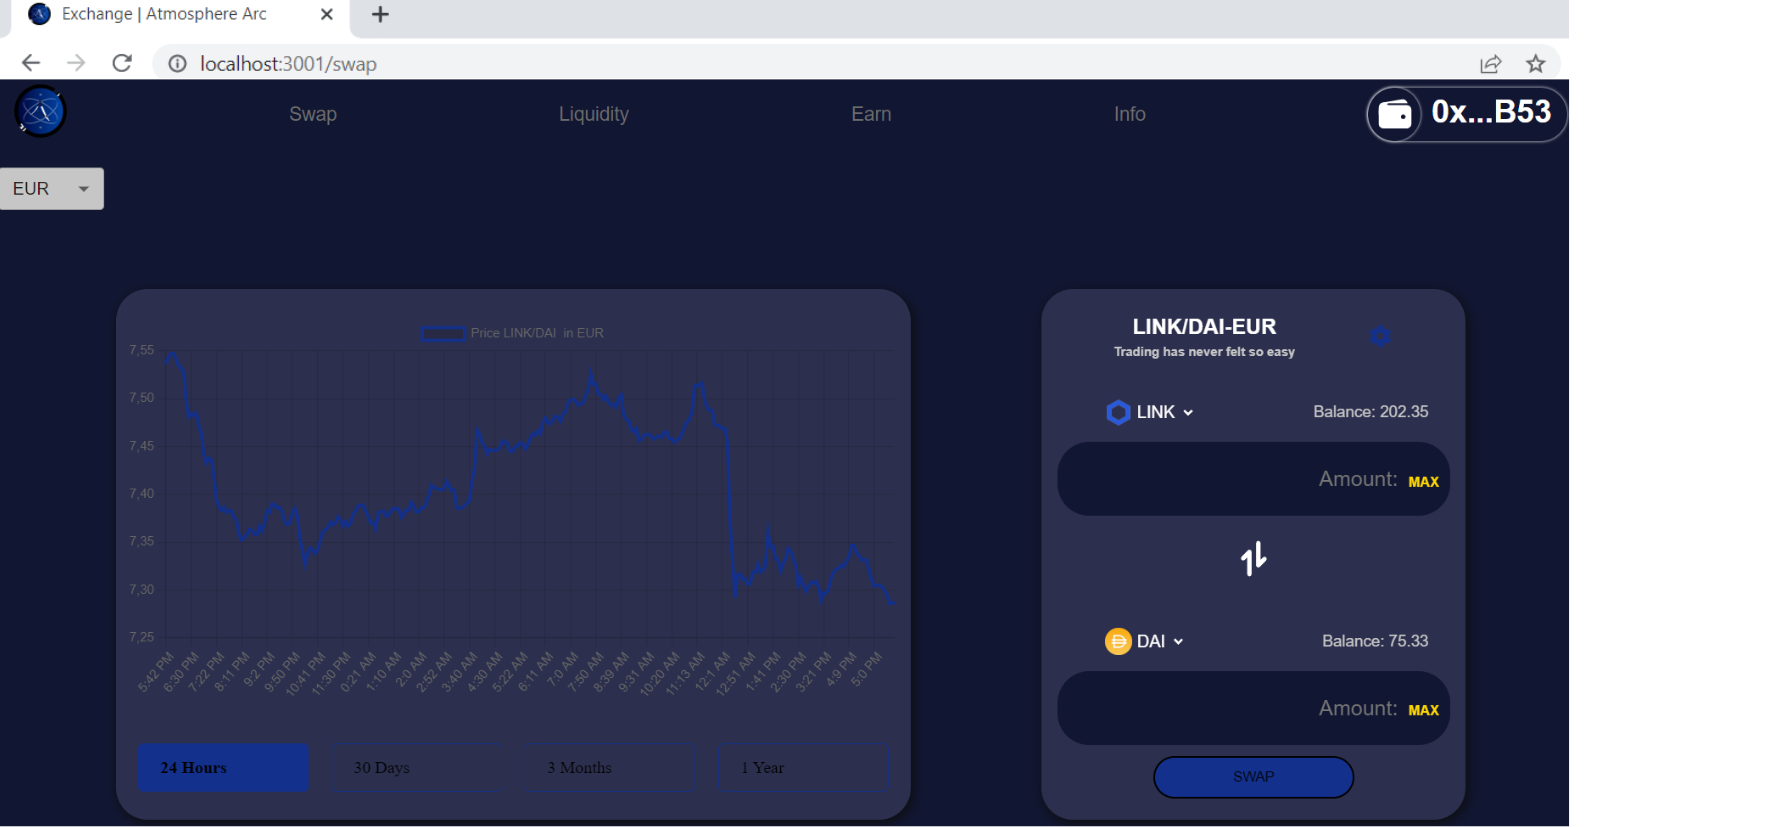
\includegraphics[width=15cm,height=7cm]{Immagini/SwapSchermata.png}
    \caption[Schermata generale dello Swap]{Schermata generale dello Swap.}
    \label{schermataSwap}
\end{figure}

\subsubsection{Componente Liquidity.js}\makeatletter\def\@currentlabel{Liquidity.js}\makeatother\label{Liquidity.js}
La componente \textcourier{Liquidity.js} è la seconda parte del nostro exchange che si occupa della gestione e della creazione dei Pool di liquidità. Il Card in questione è molto simile a quello dello swap, con l'unica differenza che la logica dietro ad esso è molto differente (le differenze verrano precisate nel dettaglio in \ref{interazione_smartc}).


\begin{figure}[h]
    \centering
    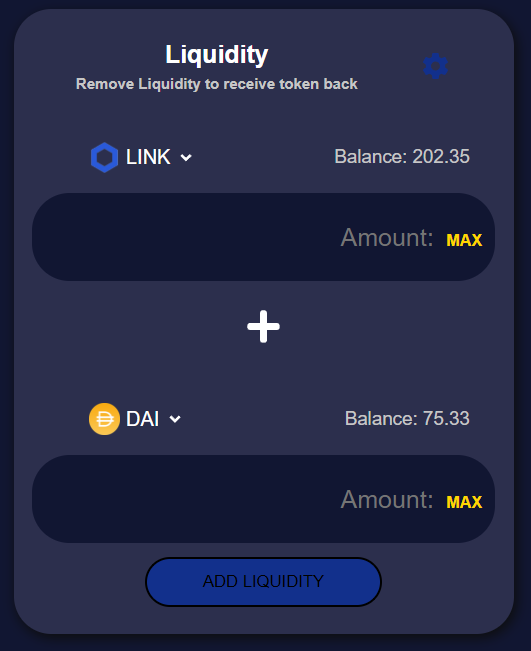
\includegraphics[width=8cm,height=9cm]{Immagini/LiquidityCard.png}
    \caption[Card per l'aggiunta di liquidità nei pool di liquidità]{Interfaccia grafica Card per l'aggiunta di liquidità nei pool di liquidità.}
    \label{liquidityCard}
\end{figure}
Per quanto riguarda l'aspetto grafico, come si vede in figura \ref{liquidityCard}, le uniche due differenze con lo swap si denotano dal bottone che avvia la logica dell'operazione (con etichetta “Add Liquidity”) e nella visualizzazione dei valori inseriti dall'utente all'interno dei due form di input.

Il form è stato pensato in maniera tale che un utente, subito dopo l'inserimento di un dato quantitativo di token (e quindi dell'ipotetica liquidità da aggiungere all'interno della Pool), il sistema calcoli gli importi massimi di output per quel determinato valore, date le \textit{riserve} per quel Pool.

L'operazione appena descritta è molto utile per visualizzare quanti token effettivi l'utente debba depositare nella Pool (ricordiamo che per depositare fondi in un Pool, è necessario fornire una stessa quantità di liquidità per token, come anticipato nel paragrafo \ref{pool_liquidità}).

Questo è reso possibile grazie ad una funzione scritta in \textcourier{Liquidity.js}, mostrata di seguito:

\begin{lstlisting}[caption={[\textcourier{getPriceLiquidity()} Function]},language=jsx] 
const getPriceLiquidity = async (value) => {
const utilsSet = async (convertion) => {
    if (PairAddress === NULL_ADDRESS) {
       const valueConverted=convertToWei(convertion,value)
       setTokenA_Quantity(valueConverted)
    }
    else {
       /*flag booleano (loading) per attendere che
       l'operazione a riga 16 termini. Utilizzata per 
       visualizzare un loading animation durante l'esecuzione*/
       setLoading(true) 
       const valueConverted=convertToWei(convertion,value)
       setTokenA_Quantity(valueConverted)
       const path = [
           tokenA.address,
           tokenB.address
        ]
       /*Chiamata alla funzione getAmountsOut() dallo
       smart-contract del Router dell'exchange*/
       const price = 
       await props.router.methods.
       getAmountsOut(tokenA_Quantity, path).call()
       const output = props.web3.utils.fromWei(price[1], "ether")
       setLoading(false)
       setOutputQuantity(output)
   }
}
const PairAddress=
await props.factory.methods.
getPair(tokenA.address, tokenB.address).call();
setPairAddress(PairAddress);
// Se i due token sono stati selezionati
if (tokenA && tokenB && value !== 0) {
    if (tokenB.decimals === 18) {
        await utilsSet("ether")
    }
    if (tokenB.decimals === 8) {
        await utilsSet("gwei")
    }
    if (tokenB.decimals === 6) {
         await utilsSet("mwei")
    }
}
}
    																			     -getPriceLiquidity
\end{lstlisting}\makeatletter\def\@currentlabel{getPriceLiquidity()}\makeatother
\label{getPriceLiquidity}

Nella funzione \textcourier{\ref{getPriceLiquidity}}, a seconda del tipo di token per il quale si deve calcolare l'importo massimo di output, viene lanciata la funzione \textcourier{utilsSet()}, la quale, da riga 7,  converte il valore del token A dato in input dall'utente nel formato del token B scelto per poi eseguire, alla riga 15 la funzione che ci permette di calcolare l'output atteso.
La funzione in questione (\textcourier{getAmountsOut()}) fa parte del \textit{RouterContract} dell'exchange e richiede come parametri un valore (corrispondente al valore inserito dall'utente nel primo form di input) e un array di address, il quale deve contenere gli address dei token scelti dall'utente per i quali si vuole aggiungere liquidità (inizializzato, nel nostro caso, a riga 11). L'array in questione può essere personalizzato a proprio piacimento per applicare il concetto di \ref{Routing}.

\subsection{Interazione con gli smart-contract}\label{interazione_smartc}
Come definito in \cite{web3API}, per l'interazione con gli smart-contract lato front-end ci viene in soccorso l'oggetto \textcourier{web3.eth.Contract}. Questo oggetto (presente all'interno del pacchetto \textcourier{web3.eth}) semplifica molto l'interazione con gli smart-contract sulla Blockchain di Ethereum. Al momento della creazione dell'oggetto \textcourier{web3.eth.Contract}, bisogna passare come primo parametro l'interfaccia JSON(corrispondente all'ABI del contratto; la definizione è stata anticipata in \ref{Solidity}) del rispettivo contratto e, come secondo parametro, l'address dello stesso. Si mostra di seguito un esempio pratico.
\begin{quote}
\centering
\textcourier{\textcolor{orangeWords}{new} \textcolor{purpleWords}{web3}.\textcolor{purpleWords}{eth}.\textcolor{yellowFunction}{Contract}(jsonInterface, address)}
\end{quote}

In questo paragrafo spiegheremo il modo con cui utilizzare l'oggetto appena citato e i vari metodi degli smart-contract da chiamare. Suddivideremo il paragrafo in diverse sezioni:
\begin{itemize}
\item Interazione con gli \ref{ERC-20 Contracts};
\item Interazione con il \ref{Exchange Contracts} (operazioni per lo swap di token e per la gestione dei Pool di liquidità).
\end{itemize}

\subsubsection{ERC-20 Contracts}\makeatletter\def\@currentlabel{ERC-20 Contracts}\makeatother
\label{ERC-20 Contracts}
Ricordiamo come lato front-end, una volta renderizzati i Card relativi allo swap e ai Pool di liquidità, venisse richiesta la selezione, da parte dell'utente, della coppia dei token. La selezione dei due token avviene attraverso le componenti \textcourier{TokenA.js} e \textcourier{TokenB.js}, che renderizzano il menu (raffigurato in figura \ref{swapCard}) e istanziano un oggetto \textcourier{web3.eth.Contract} per ogni token selezionato dall'utente.
La gestione dell' ERC-20 Contract è mostrata nello snippet di codice \ref{TokenConversion}, riportiamo la riga corrispondente dell'istanziamento:
\begin{quote}
\centering
\textcourier{\textcolor{orangeWords}{new} \textcolor{purpleWords}{web3}.\textcolor{purpleWords}{eth}.\textcolor{yellowFunction}{Contract}(ERC20abi, token.\textcolor{purpleWords}{address})}
\end{quote}
Siccome ERC-20 introduce uno standard per i token fungibili, al momento della creazione dello smart-contract riferito al token selezionato, passiamo come primo parametro l'ABI standardizzato (uguale per tutti), mentre, come secondo parametro inseriamo l'address del token scelto.

Come si può notare dal codice, l'address viene recuperato da un oggetto “token”, prelevato effettuando il map da un file JSON precedentemente compilato con la lista dei nomi di tutti i tokek, i decimals riferiti allo specifico token, l'address, il simbolo (l'acronimo del nome , ad esempio ETH per Ethereum) e un asset(l'immagine del token). Così facendo, rendiamo il codice usabile, facile da modificare con un'interfaccia grafica (il menu dei token mostrato in figura\ref{swapCard}) intuitiva e molto semplice da utilizzare per l'utente finale.

\subsubsection{Exchange Contracts}\makeatletter\def\@currentlabel{Exchange Contracts}\makeatother
\label{Exchange Contracts}

La maggior parte degli exchange decentralizzati basati sul meccanismo degli Automatic Market Maker (AMM), come la nostra applicazione, possiede, solitamente , due smart-contract principali:

\begin{itemize}
\item \textit{Factory Contract}: sono presenti le funzioni che permettono la generazione dei Pool di liquidità. Ogni Pool è identificabile da un \textit{Pair Contract} che definisce la coppia dei token. Nella nostra applicazione prende il nome di \textit{AtmosFactory};
\item \textit{Router Contract}: supporta le funzionalità di base svolte per interagire con i \textit{Pair Contract}, fornisce una serie di funzioni di visualizzazione che verranno ampiamente utilizzate sul frontend del DEX e si interpone tra l'utente e il \textit{Factory Contract}. Nella nostra applicazione prende il nome di \textit{AtmosRouter}.
\end{itemize}

In questa parte dell'elaborato tratteremo la logica che c'è dietro alle operazioni che la nostra Dapp ci permette di fare, passando dalle operazioni di swap, fino all'aggiunta della liquidità per un Pool.
Per quanto riguarda le operazioni di swap, nel nostro caso si sono diverse funzioni specifiche del \textit{Router Contract}; la prima funziona implementata è \textcourier{ \ref{swapExactTokensForTokens}}, il codice, scritto in Solidity, viene mostrato di seguito:\\

\begin{lstlisting}[caption={[\textcourier{swapExactTokensForTokens()} Function]},language=Solidity] 
function swapExactTokensForTokens(
        uint256 amountIn, uint256 amountOutMin,
        address[] calldata path, address to,
        uint256 deadline
    ) external virtual override 
    ensure(deadline) returns (uint256[] memory amounts) {
        amounts = 
        AtmosLibrary.getAmountsOut(factory, amountIn, path);
        require(amounts[amounts.length - 1] >= amountOutMin,
        "AtmosRouter: INSUFFICIENT_OUTPUT_AMOUNT");
        
        TransferHelper.safeTransferFrom(
            path[0],
            msg.sender,
            AtmosLibrary.pairFor(factory, path[0], path[1]),
            amounts[0]
        );
        _swap(amounts, path, to);
    }    															
    															   	  -swapExactTokensForTokens
\end{lstlisting}\makeatletter\def\@currentlabel{swapExactTokensForTokens()}\makeatother
\label{swapExactTokensForTokens}

Come mostrato all'interno dello snippet, la funzione richiede cinque parametri distinti:

\begin{itemize}
\item \textit{amountIn} corrispondente alla quantità di token da inviare;
\item \textit{amountOut}, ossia la quantità minima di token di output che deve essere ricevuta;
\item Il \textit{path}, ossia il “sentiero” che la funzione deve percorrere attraverso i pool di liquidità. Questi ultimi devono avere liquidità al loro interno;
\item Il \textit{destinatario} dei token che verranno mandati;
\item La \textit{deadline}, cioè la scadenza dopo la quale la transazione verrà ripristinata.
\end{itemize}

L'\textit{omountIn} corrisponde all'importo di token inserito nel form di input mostrato in figura \ref{swapCard}, cioè il valore che l'utente decide di trasferire a seconda delle sue disponibilità.
L'\textit{amountOut} viene settato a zero per garantire il corretto funzionamento (non si è pensata a nessuna limitazione).
Il \textit{path} viene settato attraverso l'address dei due token scelti dall'utente nel Card dello swap.

Il \textit{destinatario} dell'invio corrisponderà all'account in quel momento connesso alla Dapp, mentre la \textit{deadline} è settata al momento del timestamp più dieci minuti di tolleranza nei quali l'utente deve completare e confermare la transazione.
La precitata funzione scambia una quantità esatta di token (previa approvazione di un importo di indennità da dare al \textit{Router}, vedere \ref{approve}) di input con il maggior numero possibile di token di output, lungo il percorso determinato dal parametro \textcourier{path}. Il primo elemento del percorso deve essere il token che si vuole scambiare, l'ultimo deve essere il token di output che si vuole ricevere e tutti gli elementi intermedi, invece, rappresentano coppie intermedie tramite cui scambiare (guardare il \textit{Custom Path} di \ref{Routing}).

A riga 8, attraverso la funzione \textcourier{getAmountsOut()} (la spiegazione di questa funzione è stata anticipata in \textcourier{\ref{getPriceLiquidity}},) si ricava l'omount calcolato dalle riserve della pool specifica per il nostro \textcourier{path}; una volta fatto ciò si trasferiscono, attraverso la funzione \textcourier{safeTransferFrom()}, i token del pool da un indirizzo all'altro. Essa richiede come parametri l'address del mittente, del ricevente, del Pair riferito alla coppia di token e l'amount definito precedentemente.
Sarà poi la funzione \textcourier{\_swap()} a completare l'operazione in via definitiva.
Si mostra lo snippet di codice presente all'interno della componente React \textcourier{Swap.js} per l'interazione allo smart-contract del \textit{Router}, la gestione della chiamata alla funzione \textcourier{\ref{swapExactTokensForTokens}} e dei relativi parametri.

\begin{lstlisting}[caption={[Call \textcourier{swapExactTokensForTokens} Function (front-end) ]},language=jsx] 
/*[...]*/
    const path = [
      tokenA.address,
      tokenB.address
    ]
    const deadline = Math.floor(Date.now() + (10 * 60))
    const valueConverted = new BN(value)
    setTokenA_Quantity(valueConverted)
       try {
//Metodo del contratto AtmosRouter.sol per lo swap di token
        await props.router.methods.swapExactTokensForTokens(
          valueConverted,
          new BN(0),
          path,
          props.currentAccount,
          deadline
        ).send({from: props.currentAccount, gas: 500000})
        .then(tx => {
             console.log("swapExactTokensForToken tx: ", tx)
        });
       } catch (error) {
            console.log(error)
       }
/*[...]*/
                                                                                          -swapExactTokensForTokens(front-end)
\end{lstlisting}\makeatletter\def\@currentlabel{swapExactTokensForTokens()}\makeatother
\label{swapExactTokensForTokens(front-end)}

Ricordiamo come l'istanza del \textit{Router Contract} venga settata al momento dell'\ref{onLogin}, ogniqualvolta un nuovo utente accede all'applicazione. La chiamata riferita al contratto viene eseguita alla riga 11, utilizzando la funzione \textcourier{send()} la quale, a differenza della funzione \textcourier{call()} vista fin ora, altera lo stato dello smart-contract richiedendo un input all'utente per essere completate.
La suddetta funzione permette di inserire dei parametri opzionali, ma molto importanti; nel nostro caso, come scritto a riga 17, si definiscono i parametri \textcourier{from} e \textcourier{gas}.
Il parametro \textcourier{from} è un address che rappresenta l'indirizzo da cui deve essere inviata la transazione, mentre il parametro \textcourier{gas} corrisponde al gas limite previsto per questa transazione. 
I parametri della funzione \textcourier{swapExactTokensForTokens} vengono inizializzati dalla riga 2 alla riga 8.


La seconda funzione implementata si tratta di  \textcourier{\ref{swapExactETHForTokens}}; di seguito viene mostrato il codice Solidity in questione:\\

\begin{lstlisting}[caption={[\textcourier{swapExactETHForTokens()} Function]},language=Solidity] 
function swapExactETHForTokens(
        uint256 amountOutMin,
        address[] calldata path,
        address to,
        uint256 deadline
    )external payable virtual override 
    
    ensure(deadline) returns (uint256[] memory amounts) {
        require(path[0] == WETH, "AtmosRouter: INVALID_PATH");
        amounts = 
        AtmosLibrary.getAmountsOut(factory, msg.value, path);
        require(amounts[amounts.length - 1] >= amountOutMin, 
        "AtmosRouter: INSUFFICIENT_OUTPUT_AMOUNT");
        IWETH(WETH).deposit{value: amounts[0]}();
        assert(IWETH(WETH).transfer(AtmosLibrary
        .pairFor(factory, path[0], path[1]), amounts[0]));
        _swap(amounts, path, to);
    }    											        	   -swapExactETHForTokens
\end{lstlisting}\makeatletter\def\@currentlabel{swapExactETHForTokens()}\makeatother
\label{swapExactETHForTokens}

La logica di questa funzione è molto simile alla precedente , con l'unica differenza che si scambia una quantità esatta di ETH con il maggior numero possibile di token di output; quindi, se un utente lo desidera, ha la possibilità di utilizzare Ether per lo scambio.
La funzione richiede quattro parametri:
 
 \begin{itemize}
\item {amountOutMin} come per \textcourier{swapExactTokensForTokens};
\item Il {path} corrispondente al percorso dei pool di liquidità, il primo elemento del percorso in questione deve necessariamente essere WETH\footnote{WETH (o Wrapped Ether) è un tipo speciale di token ERC-20 il cui scopo è facilitare diverse operazioni di scambio nell'ecosistema Ethereum(principalmente scambi di Ether per altri gettoni ERC-20).} e l'ultimo il token di output;
\item Il {destinatario} dei token che verranno mandati;
\item La {deadline} come per \textcourier{swapExactTokensForTokens}.
 \end{itemize}
 
 La funzione sopraccitata ha un funzionamento molto simile alla funzione \textcourier{\ref{swapExactTokensForTokens}}, con l'unica differenza che (dalla riga 14), viene richiesto il trasferimento di un numero equivalente all'amounts settato a riga 10 di WETH nella pool riferita al \textit{Pair} della coppia WETH-tokenB, per poi concludere con la consueta chiamata a \textcourier{\_swap()} e completare l'operazione in via definitiva.
 
 
 Per quanto riguarda l'interfacciamento smart-contract alla funzione appena descritta, la logica è praticamente la stessa di \textcourier{\ref{swapExactTokensForTokens(front-end)}}
 con la differenza che il \textit{path} deve essere inizializzato con l'address dei WETH riferiti alla rete di test Ropsten (nel nostro caso specifico). Di seguito mostriamo il codice presente all'interno della componente \textcourier{Swap.js}:\\

\begin{lstlisting}[caption={[Call \textcourier{swapExactETHForTokens()} Function (front-end) ]},language=jsx] 
/*[...]*/
const WETH = await props.router.methods.WETH().call()
const path = [
   WETH,
   tokenB.address
]
const deadline = Math.floor(Date.now() + (10 * 60))
const valueConverted = new BN(value)
setTokenA_Quantity(valueConverted)
     try {
//Metodo del contratto AtmosRouter.sol per lo swap di token
       await props.router.methods.swapExactETHForTokens(
             valueConverted,
             new BN(0),
             path,
             props.currentAccount,
             deadline
       ).send({from: props.currentAccount, gas: 500000})
       .then(tx => {
                    console.log("swapExactETHForTokens tx: ", tx)
                });
        } catch (error) {
            console.log(error)
}
/*[...]*/
                                                                                             -swapExactETHForTokens(front-end)
\end{lstlisting}\makeatletter\def\@currentlabel{swapExactETHForTokens()}\makeatother
\label{swapExactETHForTokens(front-end)}

Come si può notare alla riga 2 viene prelevato l'address del token WETH attraverso una chiamata dello smart-contract del \textit{Router}: \textcourier{WETH()}. Il valore risultante viene inserito nella prima posizione del percorso, nella variabile \textcourier{path}, come anticipato in precedenza. Per il resto, l'assegnazione, l'invio della transazione e la chiamata della funzione restano identici.

Da precisare come queste non siano le uniche due funzioni (per le operazioni di swap) presenti all'interno dello smart-contract del \textit{Router}, bensì ne sono presenti diverse per ogni necessità. La logica di queste altre funzioni restano molto simili, con l'unica differenza che l'ordine con cui i percorsi vengono assegnati cambia, esempi di funzioni sono: \textcourier{swapTokensForExactTokens()} (il quale riceve una quantità esatta di token di output e non di input),\textcourier{swapExactTokensForETH()} (il quale permette di \textit{ricevere} ETH invece di mandarli).

Una volta discusso delle funzioni riferite allo swap dei token, parliamo di una delle funzioni più importanti di un DEX, ossia quella per l' \ref{_addLiquidity}.
La seguente funzione viene mostrata di seguito:\\

\begin{lstlisting}[caption={[\textcourier{\_addLiquidity()} Function]},language=Solidity] 
function _addLiquidity(
        address tokenA,address tokenB,uint256 amountADesired,
        uint256 amountBDesired,uint256 amountAMin,uint256 amountBMin
    ) internal virtual returns
    (uint256 amountA, uint256 amountB) {
    /* Creazione del Pair Contract se non esiste */
   if (IAtmosFactory(factory)
   .getPair(tokenA, tokenB) == address(0)) {
       IAtmosFactory(factory).createPair(tokenA, tokenB);
   }
   
    /*Se si e' primi ad aggiungere liquidita' 
    si determinera' il prezzo iniziale del Pool*/
(uint256 reserveA, uint256 reserveB) = 
AtmosLibrary.getReserves(factory, tokenA, tokenB);

if (reserveA == 0 && reserveB == 0) {
            (amountA, amountB) = 
            (amountADesired, amountBDesired);
} 
else {
   uint256 amountBOptimal = 
   AtmosLibrary.quote(amountADesired, reserveA, reserveB);
   if (amountBOptimal <= amountBDesired) {
       require(amountBOptimal >= amountBMin,
       "AtmosRouter: INSUFFICIENT_B_AMOUNT");
  (amountA, amountB) =
  (amountADesired, amountBOptimal);
   } else {
   uint256 amountAOptimal = 
   AtmosLibrary.quote(amountBDesired, reserveB, reserveA);
   assert(amountAOptimal <= amountADesired);
   require(amountAOptimal >= amountAMin, 
   "AtmosRouter: INSUFFICIENT_A_AMOUNT");
   (amountA, amountB) =
   (amountAOptimal, amountBDesired);
            }
        }
    }    											        	   			   -_addLiquidity
\end{lstlisting}\makeatletter\def\@currentlabel{\_addLiquidity()}\makeatother
\label{_addLiquidity}

La seguente funzione ha bisogno di otto parametri, definiti di seguito:
\begin{itemize}
\item L'address del \textit{tokenA};
\item L'address del \textit{tokenB};
\item \textit{amountADesired}: la quantità di tokenA da aggiungere come liquidità;
\item \textit{amountBDesired}: la quantità di tokenB da aggiungere come liquidità;
\item \textit{amountAMin}: limita il fatto che il prezzo del tokenB/ tokenA possa aumentare prima che la transazione avvenga;
\item \textit{amountBMin}: limita il fatto che il prezzo del tokenA/ tokenB possa aumentare prima che la transazione avvenga.
\end{itemize}
Mentre, come valori di ritorno, restituisce la coppia \textcourier{(amountA,amountB)}.
A riga 7, la funzione parte con un controllo chiamando la funzione \textcourier{getPair()} del \textit{Factory Contract}. Questa funzione serve per ottenere l'indirizzo del \textit{Pair Contract} dati i due token scelti dal front-end. Tramite questa funzione, si verifica se è uguale ad un adress nullo; se sì, viene creato il \textit{Pair Contract} corrispondente alla coppia tramite la funzione dello smart-contract della \textit{Factory} chiamata  \textcourier{createPair()}.

Subito dopo aver effettuato questo controllo preliminare, si verifica, a riga 17, se le riserve dei due token sono uguali a zero (praticamente se si è i primi a voler aggiungere liquidità) allora si aggiunge la liquidità con i valori passati in  \textcourier{amountADesired} e \textcourier{amountBDesired}, determinando, di conseguenza, il prezzo iniziale della Pool, in quanto primi Liquidity Provider (LP).

Se questo non fosse il caso, da riga 21 in poi si setta la variabile \textcourier{amountBOptimal} con la funzione \textcourier{quote()} dello smart-contract della \textit{Library}. Essa richiede tre parametri specifici: come primo parametro un importo di asset (in questo caso  \textcourier{amountADesired}) e come secondo e terzo parametro le riserve dei due token; la funzione attraverso dei calcoli matematici (mostrati di seguito):
\begin{quote}
\centering
                   \textcourier{amountBOptimal=(amountADesired $\bigcdot $ reserveB)\big/reserveA}
\end{quote}
trova l'importo ottimale del token B.

Una volta fatto ciò, a riga 24, si controlla se il valore trovato è minore o uguale della quantità di token che si vogliono aggiungere alla liquidità (\textcourier{amountBDesired}), se va a buon fine, si richiede, alla riga successiva, che tale valore sia anche maggiore o uguale a \textcourier{amountBMin}(per evitare che l'operazione non sia più conveniente) e solo se anche questa condizione è verificata verrà restituita la coppia \textcourier{(amountADesired,amountBOptimal)}.

Se, invece, la prima condizione citata a riga 24, non venisse verificata , si riesegue lo stesso identico codice, ma per il token A.

Per quanto riguarda la chiamata dell'aggiunta della liquidità da parte del front-end (appena l'utente ha inserito tutti i dati e ha interagito con il bottone,come mostrato in \ref{Liquidity.js}) si utilizza un'altra funzione sempre facente parte del \textit{Router Contract} ossia \ref{addLiquidity}: \\

\begin{lstlisting}[caption={[\textcourier{addLiquidity()} Function]},language=Solidity] 
function addLiquidity(
   address tokenA,address tokenB,
   uint256 amountADesired,uint256 amountBDesired,
   uint256 amountAMin,uint256 amountBMin,address to,
   uint256 deadline
   )external virtual override ensure(deadline)
   returns (
       uint256 amountA,
       uint256 amountB,
       uint256 liquidity
    )
    {
        (amountA, amountB) =
        _addLiquidity(tokenA, tokenB,
        amountADesired, amountBDesired,
        amountAMin, amountBMin);
        address pair = AtmosLibrary
        .pairFor(factory, tokenA, tokenB);
        TransferHelper
        .safeTransferFrom(tokenA, msg.sender, pair, amountA);
        TransferHelper
        .safeTransferFrom(tokenB, msg.sender, pair, amountB);
        liquidity = IAtmosPair(pair).mint(to);
    }    											        	   			    -addLiquidity
\end{lstlisting}\makeatletter\def\@currentlabel{addLiquidity()}\makeatother
\label{addLiquidity}

Questa è la funzione che lanceremo dal front-end, la quale possiede gli stessi identici parametri della funzione \ref{_addLiquidity}, con l'aggiunta dei parametri \textit{deadline} e \textit{to}(riferito all'address del destinatario). 
Partendo da riga 13, la funzione richiama \ref{_addLiquidity} coi relativi parametri aggiunti, per farsi restituire la coppia \textcourier{(amountA,amountB)} i quali valori verranno utilizzati poi dopo per il trasferimento 

A riga 17 viene inizializzata una variabile di tipo address tramite la funzione \textcourier{pairFor()} del \textit{Library Contract}, la quale non fa altro che calcolare l'indirizzo per una coppia senza effettuare chiamate esterne alla \textit{Factory}, per l'appunto, si passa come parametro proprio l'address della \textit{Factory} e dei due token. La variabile factory in questo contesto è una \textit{variabile globale}\footnote{variabili che possono venire usate da tutte le funzioni e dal programma principale.} dello smart-contract del \textit{Router}.

Successivamente, a riga 19 e 21, chiamiamo due volte la funzione \textcourier{safeTransferHelper()} che richiede come parametri quattro valori:

\begin{itemize}
\item L'address del token da mandare al \textit{Pair};
\item L'address del \textit{msg.sender}, ossia colui che lancia la funzione (nel nostro caso l'utente attualmente collegato alla Dapp);
\item L'address del \textit{Pair} calcolato prima;
\item L'amount (il quantitativo) del rispettivo token;
\end{itemize}

La funzione in questione viene chiamata due volte perché, come ricordiamo, quando si deve aggiungere liquidità (come anticipato in \ref{pool_liquidità}), è necessario fornire la stessa quantità di liquidità per token. Proprio per questo si utilizza in \ref{_addLiquidity} la funzione \textcourier{quote()} per il calcolo del valore preciso da assegnare ai due token.
La funzione \textcourier{safeTransferHelper()}, quindi, permette di far mandare un quantitativo preciso di token al contratto \textit{Pair} da parte dell'utente chiamante.

Una volta descritte le funzioni utilizzate nel linguaggio Solidity, analizziamo come ci si è comportati, lato front-end per la chiamata della funzione per l'aggiunta della liquidità.

Di seguito si mostra lo snippet di codice di riferimento:\\

\begin{lstlisting}[caption={[Call \textcourier{addLiquidity()} Function (front-end)]},language=jsx] 
/*[...]*/
const addLiquidity = async (value) => {
/*Se i due token esistono e se il valore 
inserito nel form e' diverso da zero*/
if(tokenA && tokenB && value!==0) {
    const tokenAContract =
    SetERC20Contract(props.web3,tokenA.address)
    const tokenBContract =
    SetERC20Contract(props.web3,tokenB.address)
    await ApproveRouter(props.web3,props.currentAccount,
            tokenAContract,ROUTER_ADDRESS)
    await ApproveRouter(props.web3,props.currentAccount,
            tokenBContract,ROUTER_ADDRESS)
    await props.router.methods.addLiquidity(
                tokenA.address,
                tokenB.address,
                tokenA_Quantity,
                outputQuantity,
                0,
                0,
                props.currentAccount,
                Math.floor(Date.now() / 1000) + 60000 * 10
            ).send({from:props.currentAccount,gas:500000})
            .then(tx => console.log("\addLiquidity tx: "+tx))
        }
    }
/*[...]*/

/*Funzione chiamata a riga 10 e 12*/
export async function ApproveRouterSwap
(web3,currentAccount,_contract,router) {
	const value=web3.utils
    .toBN("11579208923731619542357098500868790785326
    9984665640564039457584007913129639935");
    
    await _contract.methods
        .approve(router, value)
        .send({from: currentAccount})
}
                                                                                                      -addLiquidity(front-end)
\end{lstlisting}\makeatletter\def\@currentlabel{addLiquidity()}\makeatother
\label{addLiquidity(front-end)}

La funzione in questione viene chiamata all'onClick del bottone con etichetta “addLiquidity” visualizzato in figura \ref{liquidityCard}. Prima di poter chiamare la funzione dello smart-contract del nostro \textit{Router}, bisogna inizializzare gli oggetti \textcourier{web3.eth.Contract} dei due token; a rigga 7 e 9 vengono istanziati attraverso la funzione \textcourier{SetERC20Contract()} per evitare ridondanze. 

Gli oggetti istanziati ci serviranno per lanciare la funzione \textcourier{ApproveRouter()}, la quale lancia l'\textcourier{approve()} del contratto del token passato come parametro. Un caso d'uso comune è quello di approvare i token attraverso la metodologia utilizzata in questa funzione, infatti, come si vede a riga 33, si setta una variabile con il massimo intero possibile da poter utilizzare in Solidity. Così facendo il \textit{Router Contract} può trasferire tutti i token per evitare all'utente procedure continue di approvazione, rallentando le operazioni e le procedure dei servizi offerti dal DEX. Ovviamente, prima di accettare l'approvazione di tale ammontare, l'utente deve essere consapevole dell'affidabilità della piattaforma su cui operare. Un esempio di piattaforma che utilizza questa metodologia è proprio Uniswap \cite{uniswap}.


%%%%%%%%%%%%%%%%%%%%%%%%%%%%

%%%%%%%%%%%%%%%%%%%%%%%%%%%%
\chapter{Conclusioni e sviluppi futuri}\makeatletter\def\@currentlabel{4}\makeatother
\label{cap4}
\lhead{\textbf{CAPITOLO 4.} \textit{CONCLUSIONI E SVILUPPI FUTURI}}

La sfida principale che si prepara ad affrontare la DeFi (e in generale il mondo Web3.0) è quella di diventare globale e accessibile a tutti. L'obiettivo di questo elaborato di tesi è proprio quello di realizzare una piattaforma moderna, che adopera framework e librarie innovative per la creazione di applicazioni decentralizzate, in grado di migliorare l’usabilità e la scalabilità dei servizi offerti solitamente da un'applicazione DeFi.

Per garantire che tutti gli utenti possano beneficiare dei vantaggi della finanza decentralizzata, è necessario educare le persone attraverso piattaforme di facile utilizzo. L'obiettivo è quello di offrire strumenti capaci di rendere più facile familiarizzare con la blockchain e di garantire una vera decentralizzazione con una conseguente padronanza, completa, delle proprie finanze senza avere l'obbligo e la necessità di affidarsi ad enti centrali.

Possibili sviluppi futuri possono essere diversi; sicuramente sarà importante garantire certezze all'utente attraverso la comunicazione di progetti sicuri, regolamentati in maniera chiara e trasparente. Tutto ciò aiuterebbe molto il suo riconoscimento a livello globale come vera alternativa alla finanza tradizionale. Il recente interesse che si sta avendo nel mondo delle criptovalute è sicuramente un passo avanti del processo.

In conclusione, ricordiamo, che l'elaborato esposto, oltre ad aver mostrato esempi di interfacce utente, ha avuto come primario obiettivo quello di sviluppare un exchange decentralizzato basato su smart-contract. Il lavoro di tesi in questione ha dimostrato che l'applicazione sviluppata permette agli utenti di operare su un vero sistema AMM. Allo stesso tempo, viene anche confermato come un'applicazione di questo tipo possa essere intuitiva e facile da utilizzare, capace di comunicare in maniera semplice con la blockchain e di rendere l’esperienza utente leggera e molto gradevole.
%%%%%%%%%%%%%%%%%%%%%%%%%%%%

\pagestyle{fancy}
\fancyhead{}
\phantomsection\addcontentsline{toc}{chapter}{Bibliografia}
\Urlmuskip=0mu plus 4mu
\bibliographystyle{unsrt}
\bibliography{bibliografia}

%%%%%%%%%%%%%%%%%%%%%%%%%%%%

\phantomsection\addcontentsline{toc}{chapter}{Elenco delle figure}
\hypersetup{linkcolor=black} 
\listoffigures %\listoffigures 

%%%%%%%%%%%%%%%%%%%%%%%%%%%%

\phantomsection\addcontentsline{toc}{chapter}{Elenco dei codici}
\hypersetup{linkcolor=black} 
\lstlistoflistings %\lstlistoflistings 

%%%%%%%%%%%%%%%%%%%%%%%%%%%%

\input{Dediche}
\newpage\null\thispagestyle{empty}\newpage

%%%%%%%%%%%%%%%%%%%%%%%%%%%%

\end{document}
